%%%%%%%%%%%%%%%%%%%%%%%%%%%%%%%%%%%%%%%%%%%%%%%%%%%%%%%%%%%%%%%%%%%%%%%%%%
%%%%%                         CHAPITRE 1                            %%%%%%
%%%%%%%%%%%%%%%%%%%%%%%%%%%%%%%%%%%%%%%%%%%%%%%%%%%%%%%%%%%%%%%%%%%%%%%%%%

\lhead[\fancyplain{}{\leftmark}]%Pour les pages paires \bfseries
      {\fancyplain{}{}} %Pour les pages impaires
\chead[\fancyplain{}{}]%
      {\fancyplain{}{}}
\rhead[\fancyplain{}{}]%Pour les pages paires 
      {\fancyplain{}{\rightmark}}%Pour les pages impaires \bfseries
\lfoot[\fancyplain{}{}]%
      {\fancyplain{}{}}
\cfoot[\fancyplain{}{\thepage}]%\bfseries
      {\fancyplain{}{\thepage}} %\bfseries
\rfoot[\fancyplain{}{}]%
     {\fancyplain{}{\scriptsize}}


%%%%%%%%%%%%%%%%%%%%%%%%%%%%%%%%%%%%%%%%%%%%%%%%%%%%%%%%%%%%%%%%%%%%%%%%%%
%%%%%                      Start part here                          %%%%%%
%%%%%%%%%%%%%%%%%%%%%%%%%%%%%%%%%%%%%%%%%%%%%%%%%%%%%%%%%%%%%%%%%%%%%%%%%%

\chapter{Model-based Deep Learning for Hyperspectral Image Restoration}
\label{ch:T3SC}

%==============================================================================	Summary of the chapter
\begin{tcolorbox}[colback=gray!5!white,colframe=gray!75!black]

        \paragraph{Chapter abstract:}
        Hyperspectral imaging offers new perspectives for diverse applications, ranging from the  monitoring of the environment using airborne or satellite remote sensing, precision farming, food safety, planetary exploration, or astrophysics. 
        Unfortunately, the spectral diversity of information comes at the expense of various sources of degradation, and the lack of accurate ground-truth ``clean” hyperspectral signals acquired on the spot makes restoration tasks challenging.
        In particular, training deep neural networks for restoration is difficult, in contrast to traditional RGB imaging problems where deep models tend to shine. 
        In this chapter, we advocate instead for a hybrid approach based on sparse coding principles that retains the interpretability of classical techniques encoding domain knowledge with handcrafted
        image priors, while allowing to train model parameters end-to-end without massive
        amounts of data.
        We show on various denoising benchmarks that our method is computationally efficient and significantly outperforms the state of the art.

        \vspace{1em}
        The source code is freely available at \href{https://github.com/inria-thoth/T3SC}{https://github.com/inria-thoth/T3SC}.
        
        \vspace{1em}
        The chapter is based on the following publication:

        \vspace{0.5em}

        T. Bodrito$^{*}$, A. Zouaoui$^{*}$, J. Chanussot, and J. Mairal. A trainable spectral-spatial sparse coding model for hyperspectral image restoration. In \emph{Advances in Neural Information Processing Systems (NeurIPS)}, 2021

        \vspace{0.5em}

        ($^{*}$equal contributions)
    \end{tcolorbox}

\newpage
\minitoc

\section{Introduction}

Hyperspectral (HS) imaging enables measurements of the electromagnetic spectrum of a scene on
multiple bands (typically about a hundred or more), which offers many perspectives over traditional color RGB imaging. 
For instance, the high-dimensional information present in a single pixel is sometimes sufficient to identify the signature of a particular material, which is of course infeasible in the RGB domain. 
Not surprisingly, HS imaging is then of utmost importance and has a huge number of scientific and technological applications such as remote sensing \cite{bioucas-dias_hyperspectral_2013, goetz_three_2009, manolakis_hyperspectral_2016},
quality evaluation of food products \cite{elmasry_principles_2012, feng_application_2012, liu_hyperspectral_2017}, medical imaging \cite{akbari_hyperspectral_2012, fei_chapter_2020, lu_medical_2014}, agriculture and forestry
\cite{adao_hyperspectral_2017, lu_recent_2020, mahesh_hyperspectral_2015}, microscopy imaging in biology \cite{gowen_recent_2015, studer_compressive_2012}, or exoplanet detection in astronomy \cite{gonzalez_supervised_2018}.

In this chapter, we propose a fully interpretable machine learning model for HS images
that may be seen as a hybrid approach between deep learning techniques, where parameters can be
learned end-to-end with supervised data, and classical methods that essentially rely on image priors.
Since designing an appropriate image prior by hand is very hard, our goal is to benefit from deep
learning principles (here, differentiable programming \cite{baydin_automatic_2018}) while encoding domain knowledge and physical rules about HS data directly into the model architecture, which we believe is a key to develop robust approaches that do not require massive amounts of training data.

More precisely, we introduce a novel trainable spectral-spatial sparse coding model with two layers, T3SC, which performs the following operations: (i) The first layer decomposes the spectrum measured at each pixel as a sparse linear combination of a few elements from a learned dictionary, thus performing a form of linear spectral unmixing per pixel, where dictionary elements can be seen as basis elements for spectral responses of materials present in the scene.
(ii) The second layer builds upon the output of the first one, which is represented as a two-dimensional feature map, and sparsely encodes patches on a dictionary in order to take into account spatial relationships between pixels within small receptive fields. 
To further reduce the number of parameters to learn and leverage classical prior knowledge about spectral signals \cite{wang_hyperspectral_2021}, we also assume that the dictionary
elements admit a low-rank structure -- that is, dictionary elements are near separable in the space and spectrum domains, as detailed later. 
Even though dictionary learning has been originally introduced for unsupervised learning \cite{mairal_sparse_2014, olshausen_emergence_1996}, we adopt an unrolled optimization procedure inspired by the LISTA algorithm \cite{gregor_learning_2010}, which has been very successful in imaging problems for training sparse coding models from supervised data \cite{lecouat_fully_2020, lecouat_flexible_2020, simon_rethinking_2019, xiong_smds-net_2020}.

Our motivation for adopting a two-layer model is to provide a shared architecture for different HS sensors, which often involve a different number of bands with different spectral responses. 
Our solution consists of learning sensor-specific dictionaries for the first layer, while the dictionary of second layer is shared across modalities. 
This allows training simultaneously on several HS signals, the first layer mapping input data to a common space, before processing data by the second layer.

We experimentally evaluate our HS model on standard denoising benchmarks, showing a significant
improvement over the state of the art (including deep learning models and more traditional baselines), while being computationally very efficient at test time. 
Perhaps more important than pure quantitative results, we believe that our work also draws interesting conclusions for machine learning. 
First, by encoding prior knowledge within the model architecture directly, we obtain models achieving excellent results with a relatively small number of parameters to learn, a conclusion also shared by \cite{lecouat_flexible_2020, lecouat_fully_2020} for RGB imaging; nevertheless, the effect is stronger in our work due to the scarcity of training data for HS denoising and the difficulty to train deep learning models for this task. 
Second, we also show that interpretable architectures are useful: our model architecture can adapt to different noise levels per band and modify the encoding function at test time in a principled manner, making it well suited for solving blind denoising problems that are crucial for processing HS signals.


\section{Method}

Building on Section \ref{sec:denoising} which presents some preliminaries on sparse coding and algorithm unrolling for HS image restoration, we are now in shape to introduce a trainable layer encoding both sparsity and low-rank principles.

\subsection{A Trainable Low-Rank Sparse Coding Layer}

\subsubsection{Spatial-Spectral Representation}

As shown in \cite{chakrabarti_statistics_2011, fu_adaptive_2015}, HS patches can be well reconstructed by using only a few basis elements obtained by principal component analysis. 
The authors further decompose these into a Cartesian product of separate spectral and spatial dictionaries.
In this chapter, we adopt a slightly different approach, where we consider
a single dictionary~$\D=[\dd_1, \ldots, \dd_p]$ in $\Real^{m \times p}$ as in Section~\ref{sec:denoising} with $m = c s^2$, but each element may be seen as a matrix of size $c \times s^2$ with low-rank structure. 
More precisely, we enforce the following representation:
\begin{equation}
	\label{eq:decomp}
	\forall j \in 1,\ldots,p, \quad \mathbf{d}_j = \text{vec}\left( \mathbf{U}_j \times \mathbf{V}_j\right),
\end{equation}
where $ \mathbf{U}_j$ is  in $\mathbb{R}^{s^2 \times r} $, $ \mathbf{V}_j$ is  in $\mathbb{R}^{r \times c} $, $r$ is the desired rank of the dictionary elements, and $\text{vec}(.)$ is the operator that flattens a matrix into a vector.
The hyperparameter $r$ is typically small with $r=1,2$ or $3$.  
When $r=1$, the dictionary elements are said to be separable in the spectral and spatial domains, which we found to be a too stringent condition to achieve good reconstruction in practice.

The low-rank assumption allows us to build models with a reduced number of parameters, while encoding natural assumption about the data directly in the model architecture. 
Indeed, whereas a classical full-rank dictionary $\D$ admits $cs^2p$ parameters, the decomposition~(\ref{eq:decomp}) yields dictionaries with $(s^2 + c)rp$ parameters only.
Matrices $ \mathbf{C}$ and $ \mathbf{W}$ are parametrized in a similar manner.

\subsubsection{Convolutional variant and implementation tricks}

Whereas traditional sparse coding reconstructs local signals (patches) independently according to the iterations~(\ref{eq:ISTA_C}), another variant called convolutional sparse coding (CSC) represents the whole image by a sparse linear combination of dictionary elements placed at every possible location in the image~\cite{simon_rethinking_2019}. 
From a mathematical point of view, the reconstruction loss for computing the codes $\alphab_i$ given an input image~$\mathbf y$ becomes
\begin{equation}
\label{eq:goal_csc}
\min_{\{\alphab_i \in \Real^p\}_{i=1,\ldots,n}} \frac{1}{2} \left\| \mathbf{y} - \frac{1}{m} \sum_{i=1}^{n} \mathbf{R}_i {\D} \mathbf{\alphab}_i \right\|^2 + \sum_{i=1}^n \sum_{j=1}^p \lambdab_j |{\alphab}_i[j]|.
\end{equation}

An iterative approach for computing these codes can be obtained by a simple modification of~(\ref{eq:ISTA_C}) consisting of replacing the quantity $\D \alphab_i^{(t)}$ by the $i$-th patch of the reconstructed image $\frac{1}{m} \sum_{i=1}^{n} \mathbf{R}_i {\D} \mathbf{\alphab}_i^{(t)}$.
All of these operations can be efficiently implemented in standard deep learning frameworks, since the corresponding operations corresponds to a transposed convolution with $\D$, followed by convolution with $\C$, see~\cite{simon_rethinking_2019} for more details. 
In this chapter, we experimented with the CSC variant~(\ref{eq:goal_csc}) and SC one~(\ref{eq:SC}), both with low-rank dictionaries, which were previously described. 
We observed that CSC was providing slightly better results and was thus adopted in our experiments.
Following~\cite{lecouat_fully_2020}, another implementation trick we use is to consider a different $\lambdab_j$ parameter per dictionary element, which slightly increases the number of parameters, while allowing to learn with a weighted $\ell_1$-norm in~(\ref{eq:goal_csc}).


\subsection{The Two-Layer Sparse Coding Model with Sensor-Specific Layer}
\label{subsec:vanilla}

One of the main challenge in hyperspectral imaging is to train a model that can generalize to several types of sensors, which typically admit different number of spectral bands.
Whereas learning a model that is tuned to a specific sensor is perfectly acceptable in many contexts, it is often useful to learn a model that is able to generalize across different types of HS signals.
To alleviate this issue, several strategies have been adopted such as (i) projecting signals onto a linear subspace of fixed dimension, with no guarantee that representations within this subspace can be comparable between different signals, or (ii) processing input data using a sliding window across the spectral domain.

In this chapter, we address this issue by learning a two-layer model, presented in Figure~\ref{fig:architecture}, where the first layer is tuned to a specific sensor, whereas the second layer could be generic. 
Note that the second layer carries most of the model parameters (about $20\times$ more than in the first layer in our experiments). 
Formally, let us denote by $ {\alphab}$ in $\mathbb{R}^{p \times h \times w}$ the sparse encoding of an input tensor $\mathbf{y}$ in $\mathbb{R}^{c \times h \times w}$ as previously described.
A sparse coding layer $ \Phi $ naturally yields an encoder and a decoder such that:

\begin{equation}
\Phi^{enc} : \mathbf{y}       \mapsto \mathbf{\alphab}, ~~~~\text{and}~~~~                  
\Phi^{dec} : \mathbf{\alphab}  \mapsto \frac{1}{n} \sum_{i=1}^{n} \mathbf{R}_i \mathbf{W} \mathbf{\alphab}_i. 
\end{equation}
Given a noisy image $\yy$, the denoising procedure described in the previous section with one layer can be written as 
$$ \mathbf{ \hat{x} }(\yy) = \Phi^{dec} \circ \Phi^{enc}( \mathbf{y} ). $$
Then, a straightforward multilayer extension of the procedure may consist of stacking several sparse coding layers $\Phi_1, \ldots, \Phi_L$ together to form a multilayer sparse coding denoising model:
$$ \mathbf{ \hat{x} }(\yy) = \Phi_1^{dec} \circ \cdots \circ \Phi_L^{dec} \circ \Phi_L^{enc} \circ \cdots \circ \Phi_1^{enc}( \mathbf{ y } ).$$
The model we propose is composed of two layers, as shown in Figure~\ref{fig:architecture}.
The first layer encodes spectrally the input HS image, meaning that it operates on $1 \times 1$ patches, whereas the second layer encodes both spectrally and spatially the output of the first layer.

\begin{figure}
\centering
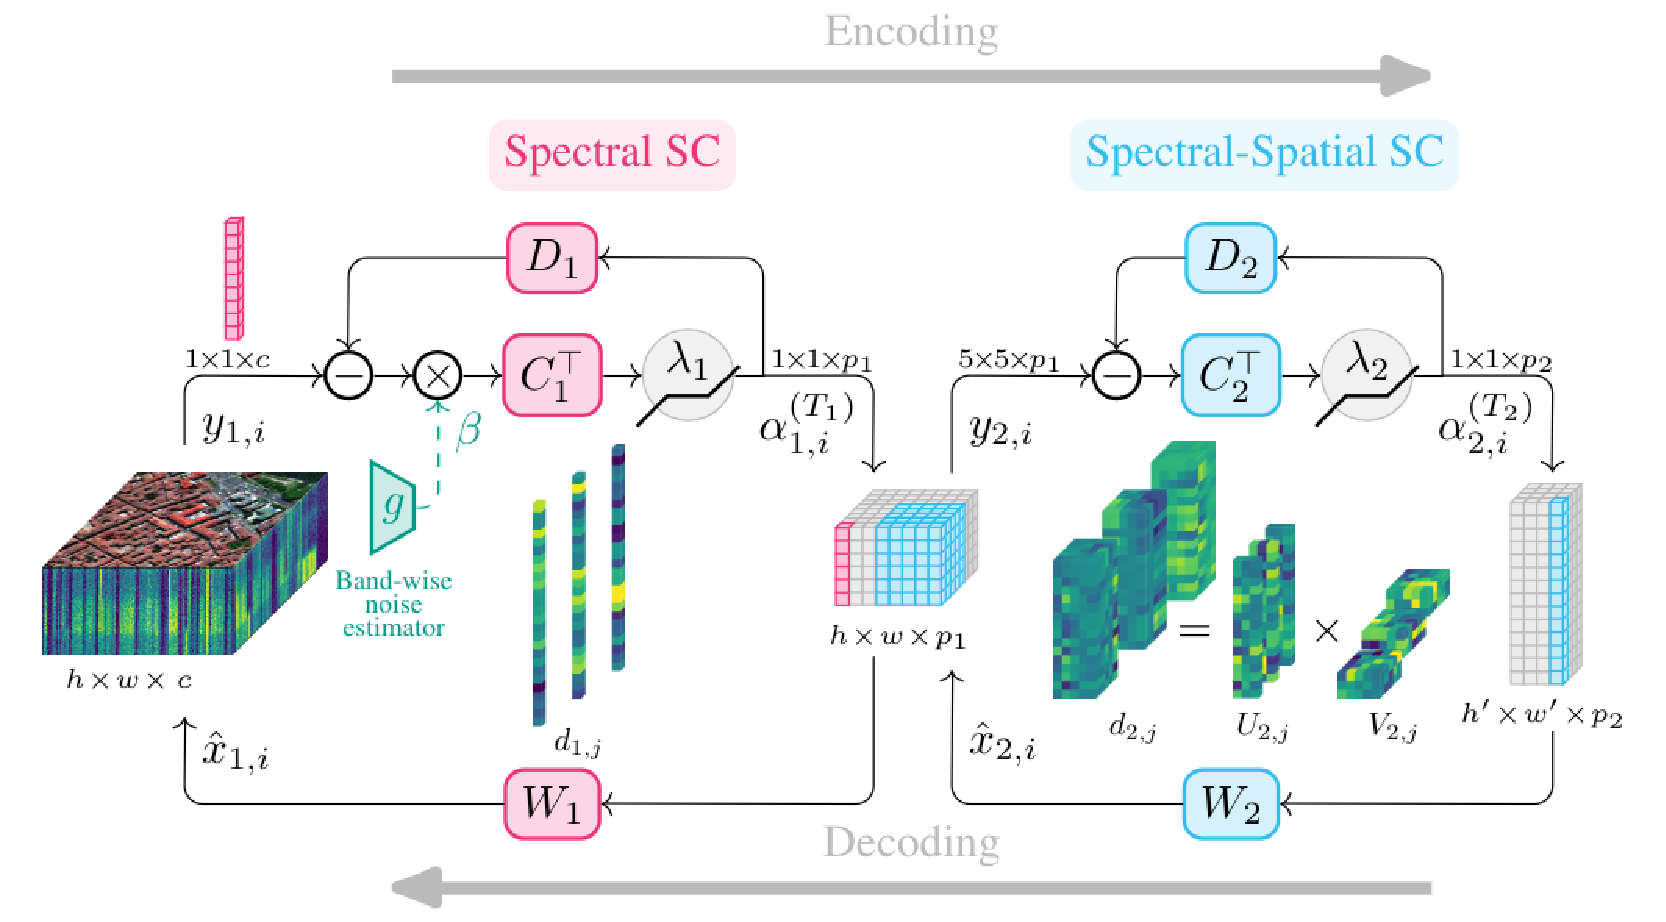
\includegraphics[width=\textwidth]{fichiers_latex/Chap1/T3SC.pdf}
\caption{Architecture of T3SC: we propose a two-layer sparse coding model which is end-to-end trainable.
The first layer performs a sensor-specific spectral decomposition, while the second layer encodes both spectral and spatial information.}
\label{fig:architecture}
\end{figure}

\subsection{Noise Adaptive Sparse Coding}
\label{subsec:adaptive}

An advantage of using a model based on a sparse coding objective~(\ref{eq:SC}) is to give the ability to encode domain knowledge within the model architecture. 
For instance, the Lasso problem~(\ref{eq:SC}) seen from a maximization a posteriori estimator implicitly assumes that the noise is i.i.d.
If the noise variance is different on each spectral band, a natural modification to the 
model is to introduce weights and use a weighted-$\ell_2$ data fitting term (which could be applied as well to the CSC model of~(\ref{eq:goal_csc})):
\begin{equation}
\label{eq:goal2}
\min_{\alphab_i \in \Real^p} \frac{1}{2} \sum_{j=1}^c \beta_j \| \mathbf{M}_j ( \mathbf{y}_i - \mathbf{D} {\alphab}_i) \|^2 + \lambda \| {\alphab}_i \|_1,
\end{equation}
where $\mathbf{M}_j$ is a linear operator that extracts band $j$ from a given HS signal. 
From a probabilistic point of view, if $\sigma_j^2$ denotes the variance of the noise for band $j$, we may choose the corresponding weight~$\beta_j$ to be proportional to $1/\sigma_j^2$.
Yet, estimating accurately $\sigma_j^2$ is not always easy, and we have found it more effective to simply learn a parametric function $\beta_j = g (\mathbf{M}_j  \mathbf{y})$---here, a very simple CNN with three layers, see supplementary material for details---which is applied independently to each band.
It is then easy to modify the LISTA iterations accordingly to take into account these weights, and learn the model parameters jointly with those of the parametric function~$g$.

\section{Experiments}

We now present various experiments to demonstrate the effectiveness of our approach for HS image denoising, but first, we discuss the difficulty of defining the state of the art in this field.  
We believe indeed that it is not always easy to compare learning-free from approaches based on supervised learning.
These two classes of approaches have very different requirements/characteristics, making one class more relevant than the other one in some scenarios, and less in others. 
Table~\ref{table:comp} summarizes their characteristics, displaying advantages and drawbacks of both approaches.
\begin{table}
   \caption{Simplified comparison between learning-free and learning-based approaches.}\label{table:comp}
   \vspace*{0.05cm}
   \centering
\begin{tabular}{llllll}
\toprule
   & \emph{Data req.} & \emph{training} & \emph{inference} &  \emph{adapt. to new data} & \emph{complex noise} \\
                  \hline
   {\bfseries learning-free}  & no req. & no training & slow & easy & poor \\
                  \hline
   {\bfseries learning-based}  & clean data & slow & fast & complicated & good perf. \\
\bottomrule

\end{tabular}
\end{table}

\subsubsection{Benchmarked models}

Keeping in mind the previous dichotomy, we choose to compare our method to traditional methods such as bandwise BM3D \cite{dabov_image_2007} (implementation based on \cite{makinen_exact_2019, makinen_collaborative_2020}), BM4D \cite{maggioni_nonlocal_2013}, GLF \cite{zhuang_hyperspectral_2017}, LLRT \cite{chang_hyper-laplacian_2017}, NGMeet \cite{he_non-local_2020}.
We also included deep learning models in our benchmark such as HSID-CNN \cite{yuan_hyperspectral_2019}, HSI-SDeCNN \cite{maffei_single_2020}, 3D-ADNet \cite{shi_hyperspectral_2021}, SMDS-Net \cite{xiong_smds-net_2020} and QRNN3D \cite{wei_3-d_2020}.
Results of HSID-CNN, HSI-SDeCNN and 3D-ADNet on Washington DC Mall (available in the Appendix) are taken directly from the corresponding papers, as the train/test split is the same.
Otherwise, the results were obtained by running the code obtained directly from the authors, except for SMDS-Net, where our implementation turned out to be slightly more effective.
Note that the same architecture for our model was used in all our experiments (see Appendix).

\subsubsection{Datasets}

We evaluate our approach on two datasets with significantly different properties.
\begin{itemize}
   \item \textit{ICVL} \cite{arad_sparse_2016}  consists of 204 images of size $1392 \times 1300$ with 31 bands. 
   We used 100 images for training and 50 for testing as in \cite{wei_3-d_2020} but with a different train/test split ensuring that similar images -- \emph{e.g.}, picture from the same scene -- are not used twice.  
   \item \textit{Washington DC Mall} is perhaps the most widely used dataset\footnote{\url{https://engineering.purdue.edu/~biehl/MultiSpec/hyperspectral.html}} for HSI denoising and consists of a high-quality image of size $1280 \times 307$ with 191 bands.  
Following~\cite{shi_hyperspectral_2021}, we split the image into two sub-images of size $600 \times 307$ and $480 \times 307$ for training and one sub-image of size $200 \times 200$ for testing. 
Even though the test image does not overlap with train images, they nevertheless share common characteristics. 
Interestingly, the amount of training data is very limited here.
\end{itemize}

Specific experiments were also conducted with the datasets APEX~\cite{itten_apex-hyperspectral_2008}, Pavia\footnote{\url{http://www.ehu.eus/ccwintco/index.php?title=Hyperspectral_Remote_Sensing_Scenes}}, Urban\cite{rickard_hydice_1993} and CAVE~\cite{yasuma_generalized_2010}, which appear in the supplementary material.



\subsubsection{Normalization}

Before denoising, HSI images are normalized to $[0,1]$.
For remote sensing datasets, we pre-compute the 2\ts{nd} and 98\ts{th} percentiles for each band, on the whole the training set.
Then, normalization is performed on train and test images by clipping each band between those percentiles before applying bandwise min-max normalization, similar to \cite{audebert_deep_2019, maffei_single_2020}.
For the close-range dataset ICVL, we simply apply global min-max normalization as in \cite{xiong_smds-net_2020, wei_3-d_2020}.

\subsubsection{Noise patterns}

We evaluate our model against different types of synthetic noise:
\begin{itemize}
	\item \textit{i.i.d Gaussian noise with known variance} $\sigma^2$, which is the same on all bands.
	\item \textit{Gaussian noise with unknown band-dependent variance}: We consider Gaussian noise with different standard deviation $\sigma_j$ for each band, which is uniformly drawn in a fixed interval. These standard deviations change from an image to the other and are unknown at test time.
	\item \textit{Noise with spectrally correlated variance}: We consider Gaussian noise with standard deviation~$\sigma_j$ varying continuously across bands, following a Gaussian curve, see details in the appendix.
	\item \textit{Stripes noise} : similar to \cite{wei_3-d_2020}, we applied additive stripes noise to 33\% of bands.
	      In those bands, 10-15\% of columns are affected, meaning a value uniformly sampled in the interval $[-0.25, 0.25]$ is added to them.
	      Moreover, all bands are disturbed by Gaussian noise with noise intensity $\sigma=25$.
\end{itemize}


\subsubsection{Metrics}

In order to assess the performances the previous methods, we used five different indexes widely used for HSI restoration, namely
\begin{itemize}
    \item Mean Peak Signal-to-Noise Ratio (MPSNR), which is the classical PSNR metric averaged across bands;
    \item Mean Structural Similarity Index Measurement (MSSIM), which is based on the SSIM metric \cite{wang_image_2004}; 
    \item Mean Feature Similarity Index Measurement (MFSIM) introduced in \cite{zhang_fsim_2011};
    \item Mean ERGAS~\cite{du_performance_2007};
    \item Mean Spectral Angle Map (MSAM)~\cite{alparone_comparison_2007}.
\end{itemize}
We use MPSNR and MSSIM in the main chapter and report the other metrics in the appendix.

\subsubsection{Implementation details}

We trained our network by minimizing the MSE between the ground truth and restored images.
For ICVL, we follow the training procedure described in \cite{wei_3-d_2020}: we first center crop training images to size $1024 \times 1024$, 
then we extract patches of size $64 \times 64$ at scales 1:1, 1:2, and 1:4, with stride 64, 32 and 32 respectively.
The number of extracted patches for ICVL amounts to 52962.
For Washington DC Mall, we do not crop training images and the patches are extracted with stride 16, 8 and 8, for a total of 1650 patches.
One epoch in Washington DC Mall corresponds to 10 iterations on the training dataset.
Basic data augmentation schemes such as $90^\circ$ rotations and vertical/horizontal flipping are performed.
Code and additional details about optimization, implementation, computational resources, are provided in the supplementary material.
As reported in Table~\ref{table:unrolling}, augmenting the number unrolled iterations improves the denoising performances at the expense of inference time.
Since the Spectral-Spatial SC layer is the most time-consuming, the number of unrolled iterations chosen for the first and second layers are 12 and 5 respectively.


\section{Discussion and Conclusion}

\subsubsection{Quantitative results on synthetic noise}

We present in Table~\ref{table:icvl} the results obtained on the ICVL dataset (results on DCMall are presented in the appendix). 
Our method uses the vanilla model of Section~\ref{subsec:vanilla} for the experiments with constant $\sigma$ or correlated noise. 
For the blind denoising experiment with band-dependent $\sigma$ or for the stripe noise experiment, we use the variant of Section~\ref{subsec:adaptive}, which is designed to deal with unknown noise level per channel.

Our supervised approach achieves state-of-the-art results (or is close to the best performing baseline) on all settings. GLF performs remarkably well given that this baseline is learning-free.

A visual result on ICVL is shown in Figure~\ref{fig:icvl} for stripes noise.
Inference times are provided in Table~\ref{table:speed}, showing that our approach is computationally efficient.

\subsubsection{Results on real noise}

We also conducted a denoising experiment on the Urban dataset, reporting a visual result in Figure~\ref{fig:urban}. 
Deep models were pre-trained on the APEX dataset, which has the same number of channels as Urban (even though the sensors are different), with band-dependent noise with $\sigma \in [0-55] $.
Please note that for this experiment we did not use Noise Adaptive Sparse Coding~\ref{subsec:adaptive} for T3SC, as it is highly dependent on the type of sensor used for training.
We show that learning-based models trained on synthetic noise are able to transfer to real data.

\subsubsection{Comments on the additional results presented in the appendix}

The appendix also contains (i) results on the DCMall dataset including additional baselines mentioned above;
(ii) error bars for parts of our experimental results in order to assess their statistical significance; (iii) an experiment when learning simultaneously on several datasets with different types of sensors showing that the second layer can be generic and effective at the same time;
(iv) additional visual results; (v)  
various ablation studies to illustrate the importance of different components of our method.
\begin{table}[t]
   \captionof{table}{Denoising performance on ICVL with various types of noise patterns. The first four rows correspond to i.i.d. Gaussian noise with fixed~$\sigma$ per band. The next three rows corresponds to a noise level that depends on the band, taken uniformly on small interval. This is a blind-noise experiment since at test time, the noise level is unknown. The last two rows correspond to the scenarios with correlated $\sigma$ across bands, and with stripe noise, respectively. See main text for details.  } \label{table:icvl}

\resizebox{\textwidth}{!}{
	\begin{tabular}{c c c c c c c c c c c}
		\toprule
		$\hspace{1pt}\sigma$ \hspace{1pt}            & Metrics    & Noisy       & BM3D        & BM4D        & GLF         & LLRT        & NGMeet                  & SMDS        & QRNN3D                  & T3SC                 \\ [0.5ex]
		\hline\hline

		\multirow{2}{*}{\hspace{5pt}  5            } & \mc{MPSNR} & \mc{34.47}  & \mc{46.17}  & \mc{48.85}  & \mc{51.25}  & \mc{51.86}  & \mc{\textbf{52.74}}     & \mc{50.91}  & \mc{48.80}              & \mc{\underline{52.62}}  \\
		                                             & \mc{MSSIM} & \mc{0.7618} & \mc{0.9843} & \mc{0.9916} & \mc{0.9949} & \mc{0.9951} & \mc{\textbf{0.9960}}    & \mc{0.9944} & \mc{0.9918}             & \mc{\underline{0.9959}}           \\
		\hline
		\multirow{2}{*}{\hspace{5pt} 25 }            & \mc{MPSNR} & \mc{21.44}  & \mc{37.86}  & \mc{39.89}  & \mc{43.16}  & \mc{43.43}  & \mc{\underline{44.74}}  & \mc{42.83}  & \mc{44.20}              & \mc{\textbf{45.38}}     \\
		                                             & \mc{MSSIM} & \mc{0.1548} & \mc{0.9269} & \mc{0.9510} & \mc{0.9695} & \mc{0.9746} & \mc{\underline{0.9796}} & \mc{0.9700} & \mc{0.9782}             & \mc{\textbf{0.9825}}    \\
		\hline
		\multirow{2}{*}{\hspace{5pt} 50 }            & \mc{MPSNR} & \mc{16.03}  & \mc{34.22}  & \mc{34.22}  & \mc{39.26}  & \mc{39.69}  & \mc{41.08}              & \mc{39.25}  & \mc{\underline{41.67}}  & \mc{\textbf{42.16}}     \\
		                                             & \mc{MSSIM} & \mc{0.0502} & \mc{0.8654} & \mc{0.8654} & \mc{0.9197} & \mc{0.9504} & \mc{0.9602}             & \mc{0.9382} & \mc{\underline{0.9655}} & \mc{\textbf{0.9677}}    \\
		\hline
		\multirow{2}{*}{\hspace{5pt} 100 }           & \mc{MPSNR} & \mc{10.85}  & \mc{30.43}  & \mc{32.47}  & \mc{34.79}  & \mc{36.39}  & \mc{\underline{37.55}}              & \mc{35.64}  & \mc{37.19}              & \mc{\textbf{38.99}}     \\
		                                             & \mc{MSSIM} & \mc{0.0144} & \mc{0.7557} & \mc{0.8155} & \mc{0.7982} & \mc{0.9182} & \mc{\underline{0.9311}}             & \mc{0.8815} & \mc{0.9140}             & \mc{\textbf{0.9439}}    \\
		\hline
		\hline
		\multirow{2}{*}{\hspace{5pt} [0-15] }        & \mc{MPSNR} & \mc{33.89}  & \mc{45.81}  & \mc{45.35}  & \mc{50.57}  & \mc{48.50}  & \mc{41.67}              & \mc{48.23}  & \mc{\underline{52.07}}  & \mc{\textbf{53.31}}    \\
		                                             & \mc{MSSIM} & \mc{0.6386} & \mc{0.9767} & \mc{0.9735} & \mc{0.9948} & \mc{0.9899} & \mc{0.9078}             & \mc{0.9900} & \mc{\underline{0.9957}} & \mc{\textbf{0.9967}}   \\
		\hline
		\multirow{2}{*}{\hspace{5pt}[0-55] }         & \mc{MPSNR} & \mc{23.36}  & \mc{39.06}  & \mc{38.43}  & \mc{44.22}  & \mc{41.13}  & \mc{32.94}              & \mc{41.76}  & \mc{\underline{47.13}}  & \mc{\textbf{48.64}}     \\
		                                             & \mc{MSSIM} & \mc{0.2601} & \mc{0.9231} & \mc{0.9074} & \mc{0.9818} & \mc{0.9580} & \mc{0.7565}             & \mc{0.9620} & \mc{\underline{0.9884}} & \mc{\textbf{0.9911}}     \\
		\hline
		\multirow{2}{*}{\hspace{5pt}[0-95] }         & \mc{MPSNR} & \mc{19.06}  & \mc{36.17}  & \mc{35.55}  & \mc{41.43}  & \mc{38.44}  & \mc{29.40}              & \mc{38.94}  & \mc{\underline{43.98}}              & \mc{\textbf{46.30}}     \\
		                                             & \mc{MSSIM} & \mc{0.1614} & \mc{0.8760} & \mc{0.8540} & \mc{0.9674} & \mc{0.9354} & \mc{0.6609}             & \mc{0.9357} & \mc{\underline{0.9753}}             & \mc{\textbf{0.9859}}    \\
		\hline
		\hline

		\multirow{2}{*}{\hspace{5pt}Corr.}           & \mc{MPSNR} & \mc{28.85}  & \mc{42.73}  & \mc{42.13}  & \mc{47.05}  & \mc{45.76}  & \mc{38.06}              & \mc{45.98}  & \mc{\underline{48.90}}  & \mc{\textbf{49.89}}    \\
		                                             & \mc{MSSIM} & \mc{0.4740} & \mc{0.9599} & \mc{0.9070} & \mc{0.9881} & \mc{0.9824} & \mc{0.8536}             & \mc{0.9835} & \mc{\underline{0.9911}} & \mc{\textbf{0.9923}}    \\
		\hline
		\hline

		\multirow{2}{*}{\hspace{5pt}Strip.}          & \mc{MPSNR} & \mc{21.20}  & \mc{34.88}  & \mc{37.70}  & \mc{42.06}  & \mc{39.38}  & \mc{39.78}              & \mc{41.98}  & \mc{\underline{44.60}}  & \mc{\textbf{44.74}}      \\
		                                             & \mc{MSSIM} & \mc{0.1508} & \mc{0.8641} & \mc{0.9198} & \mc{0.9628} & \mc{0.9258} & \mc{0.9333}             & \mc{0.9655} & \mc{\textbf{0.9806}}    & \mc{\underline{0.9805}}            \\
		\bottomrule
	\end{tabular}
}   
\end{table}


\begin{table}[t]
   \centering
  \captionof{table}{Inference time per image on ICVL with $\sigma=50$; SMDS, QRNN3D and T3SC are using a V100 GPU; BM4D, GLF, LLRT and NGMeet are using an Intel(R) Xeon(R) CPU E5-1630 v4 @ 3.70GHz. Note that unlike GLF, NGMeet, and LRRT, learning-based approaches such as QRNN3D and our approach require a training procedure, which may be conducted offline. The cost of such a training step was about 13.5 hours for our method and 19 hours for QRNN3D on a V100 GPU. }\label{table:speed}
   
\footnotesize
%\def\arraystretch{1.2}
\def\arraystretch{1.2}
\resizebox{\textwidth}{!}{
\begin{tabular}{ c c c c c c c c c}
	\toprule
	                        & BM3D        & BM4D        & GLF         & LLRT & NGMeet      & SMDS      & QRNN3D             & T3SC    \\ %[0.5ex]
	\hline\hline
  \mc{Inference time (s)} & \mc{1677} & \mc{2382} & \mc{5565} & \mc{24384}     & \mc{2686} & \mc{74.3} & \mc{\textbf{3.6}} & \mc{\underline{5.8}} \\
	\bottomrule
\end{tabular}
}

\end{table}
\begin{table}[t]
  \centering
   \captionof{table}{Impact of the number of unrolled iterations per layer on denoising performances and inference time. This experiment was carried out on ICVL with $\sigma=50$.} \label{table:unrolling}
	\def\arraystretch{1.2}
\resizebox{0.65\textwidth}{!}{
	\begin{tabular}{c | c c c c }
		\toprule
		Unrolled iterations per layer & 1     & 2     & 5     & 12    \\
		\hline
		MPSNR                         & 40.16 & 41.48 & 42.15 & 42.45 \\
		Inference time (s)            & 0.38  & 1.44  & 5.27  & 14.91 \\
		\bottomrule
	\end{tabular}
}

\end{table}


\begin{figure}[h!]
  
\newcommand{\figscale}{0.24}

\begin{subfigure}[b]{\figscale\textwidth}
      \begin{tikzpicture}[scale=\figscale]
        \node[anchor=south east,inner sep=0] at (0,0) {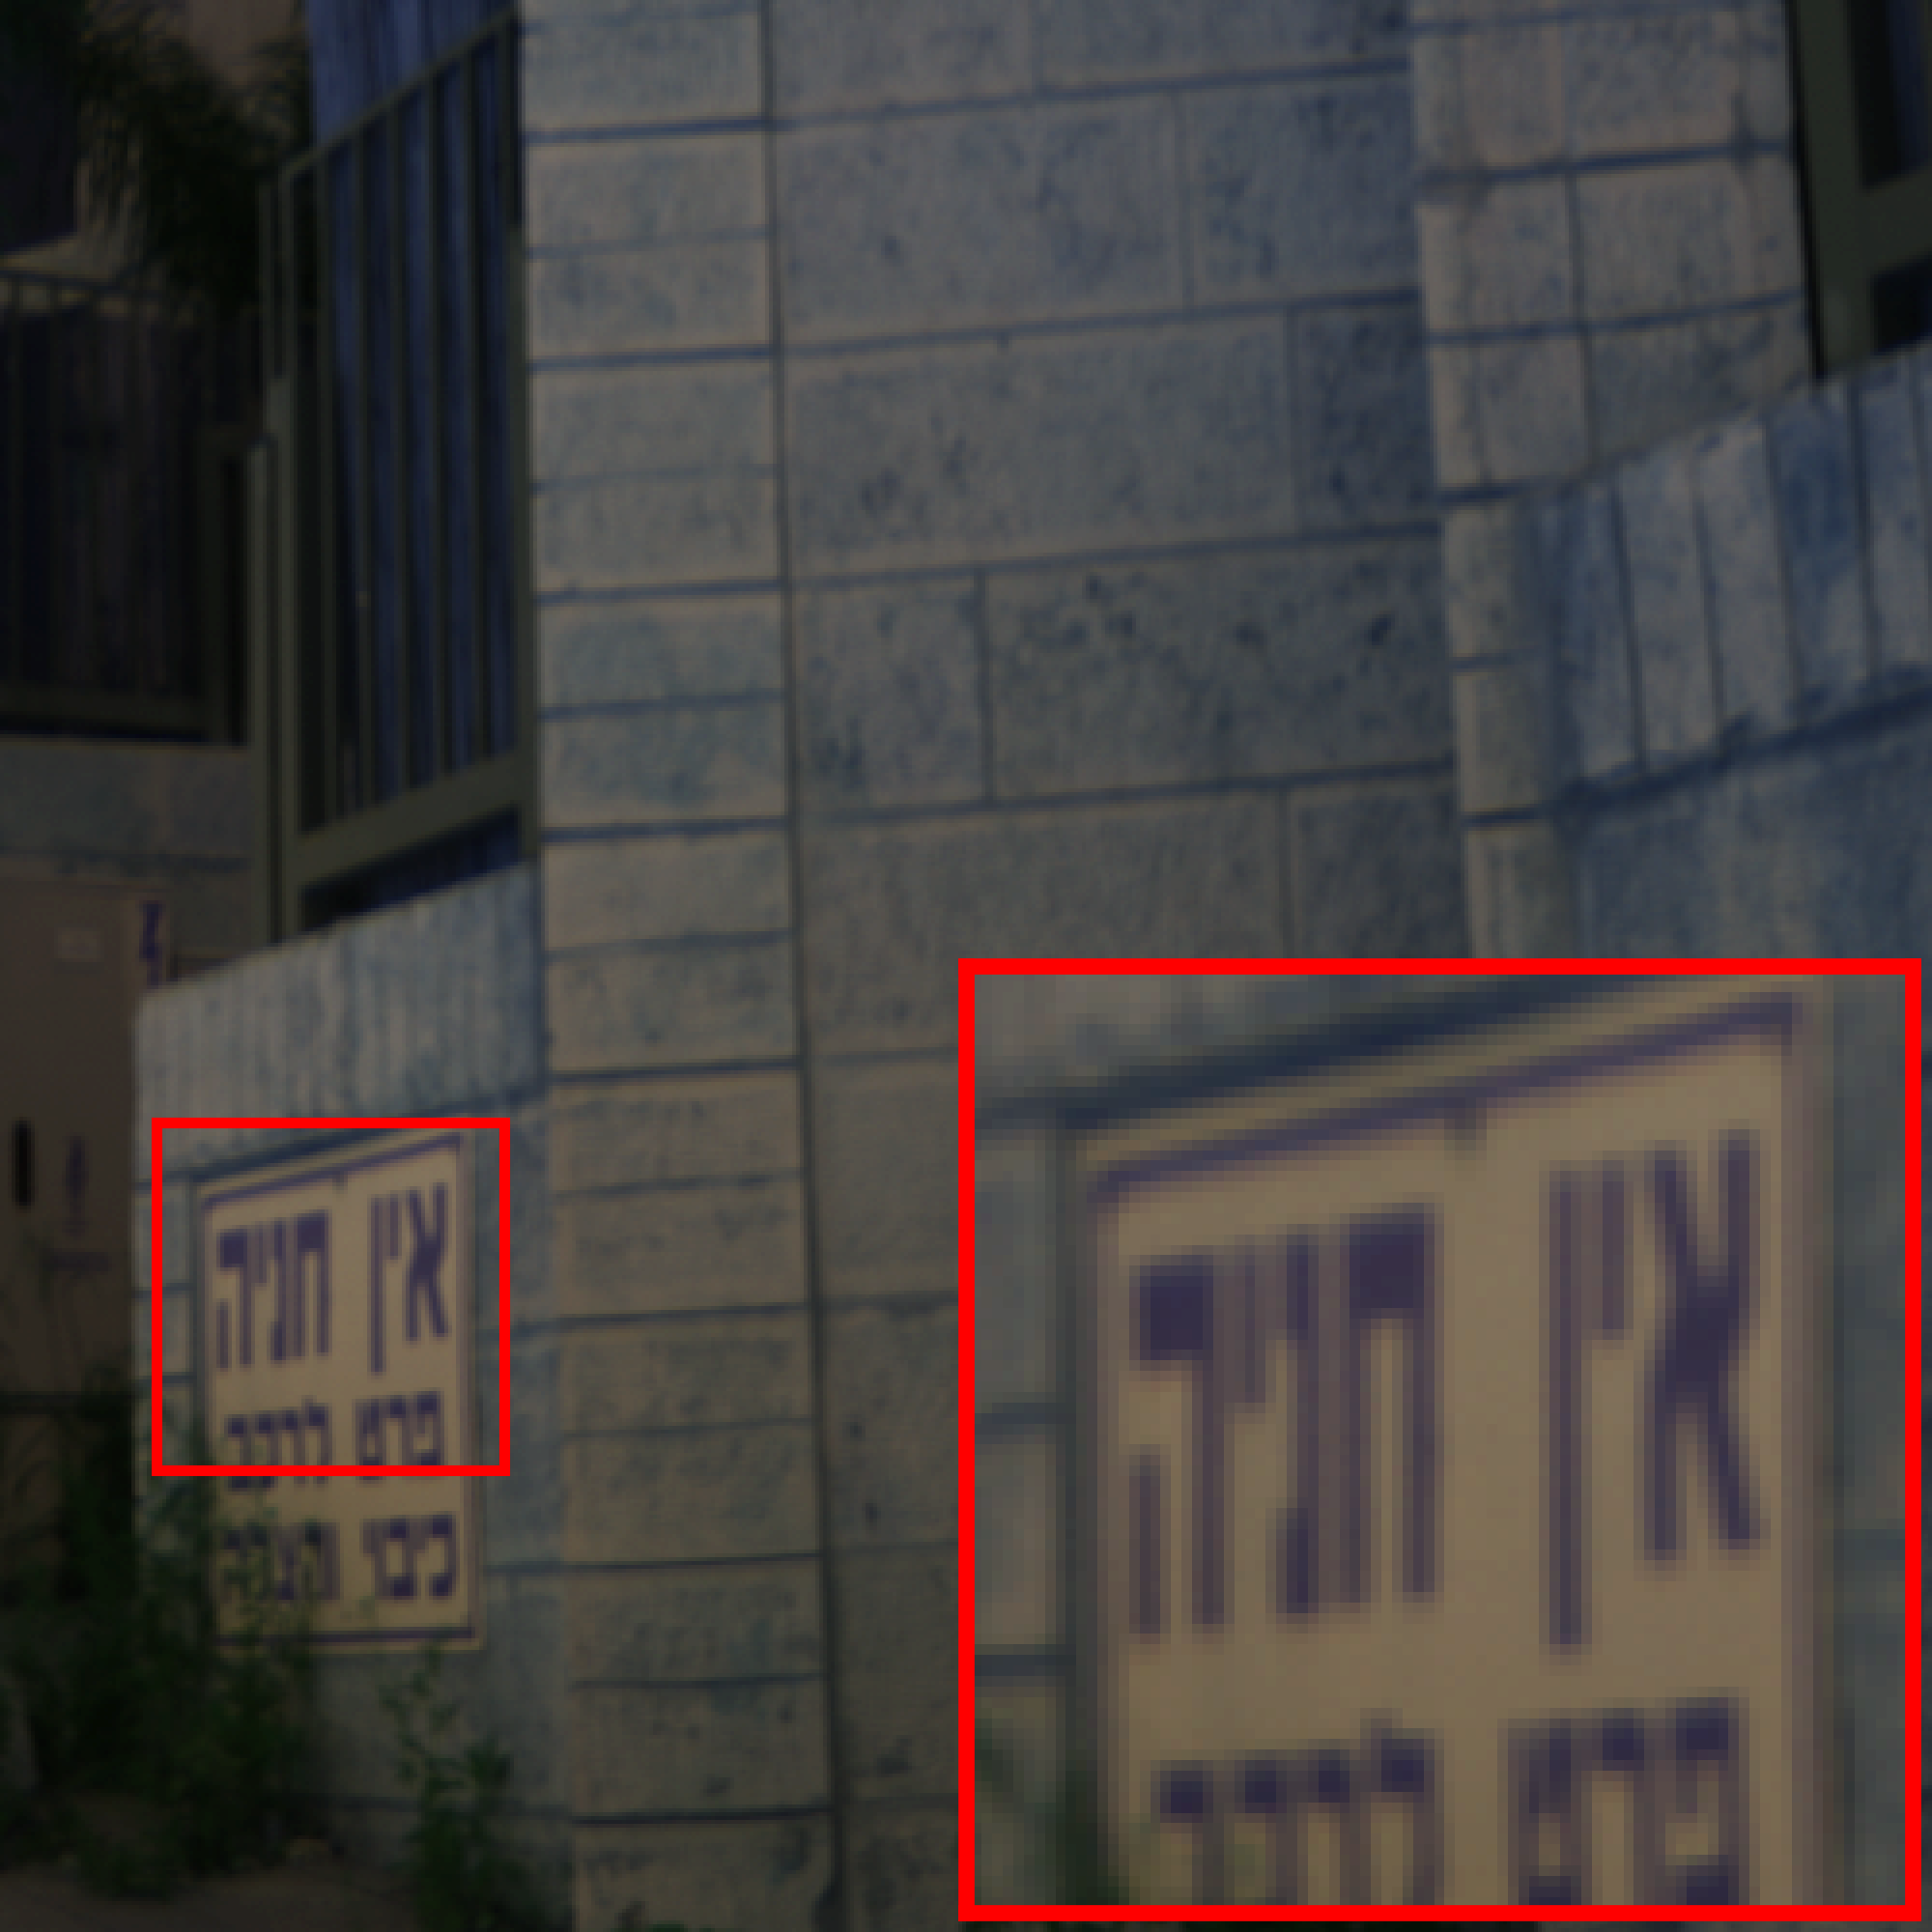
\includegraphics[width=\textwidth]{fichiers_latex/Chap1/figs/icvl_25/clean.png}};
      \end{tikzpicture}
   \caption{Groundtruth}
\end{subfigure}
\hfill
\begin{subfigure}[b]{\figscale\textwidth}
      \begin{tikzpicture}[scale=\figscale]
        \node[anchor=south east,inner sep=0] at (0,0) {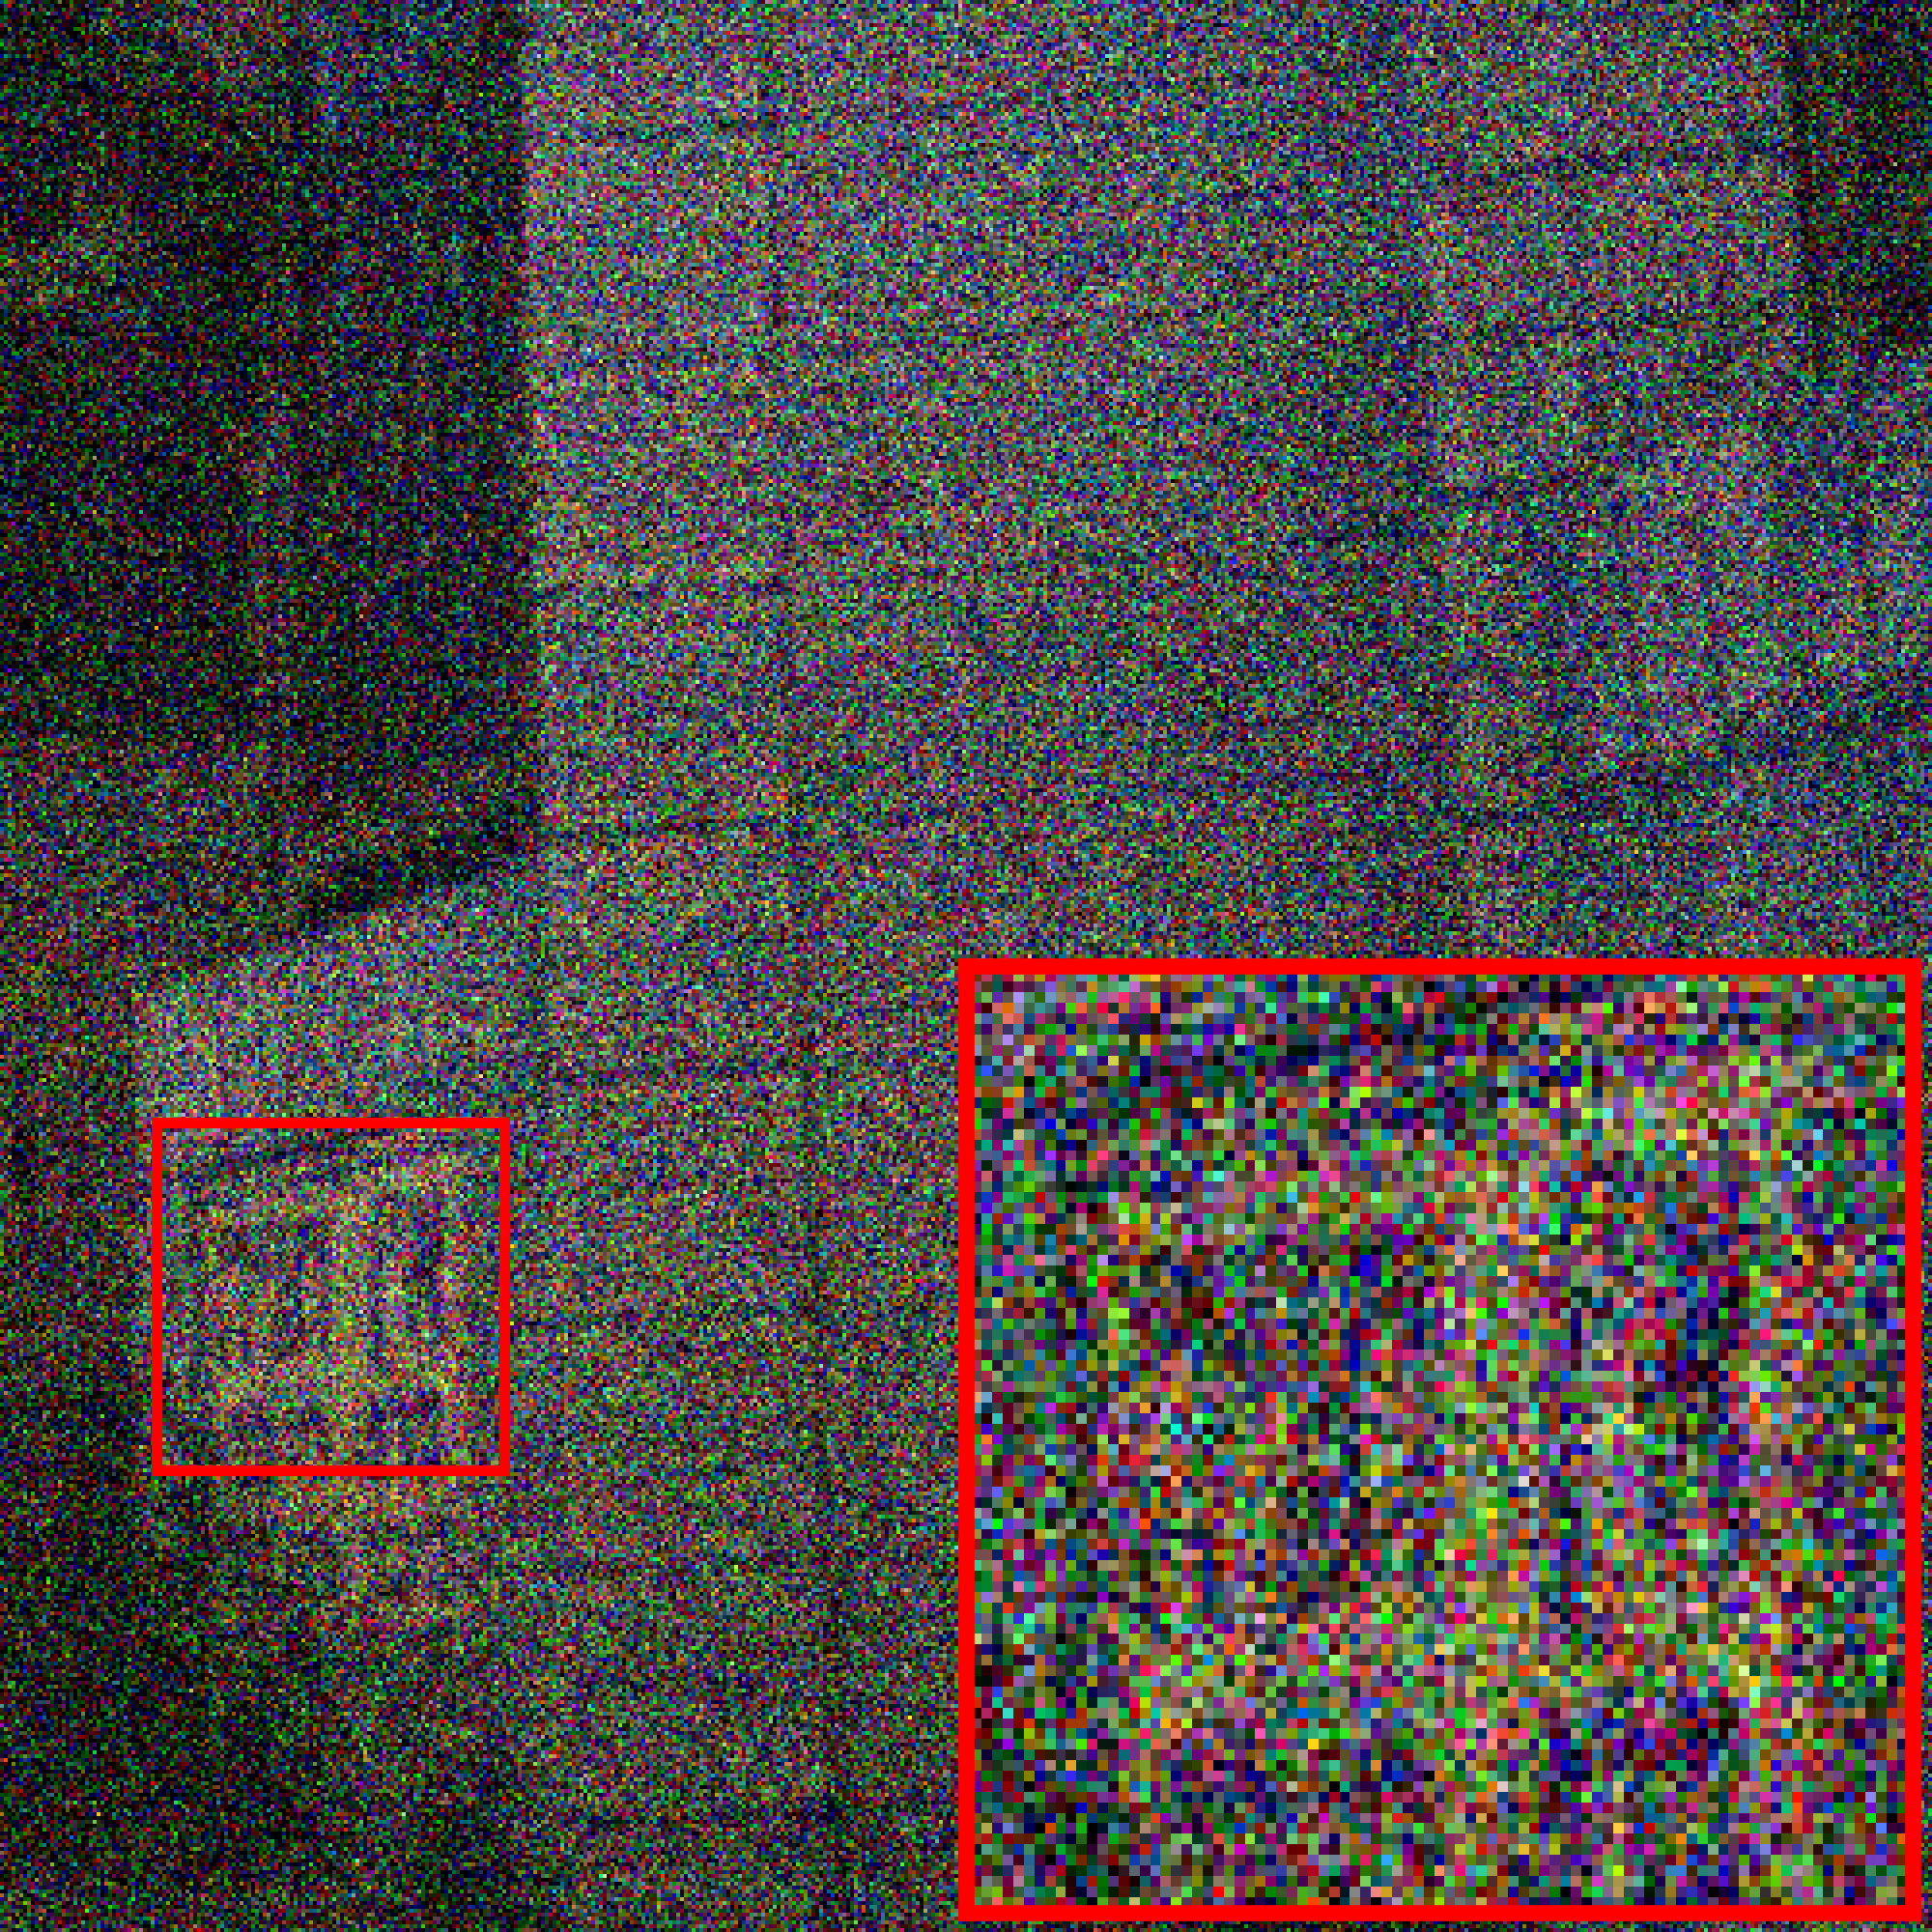
\includegraphics[width=\textwidth]{fichiers_latex/Chap1/figs/icvl_25/in.png}};
      \end{tikzpicture}
   \caption{Noisy}
\end{subfigure}
\hfill
\begin{subfigure}[b]{\figscale\textwidth}
      \begin{tikzpicture}[scale=\figscale]
        \node[anchor=south east,inner sep=0] at (0,0) {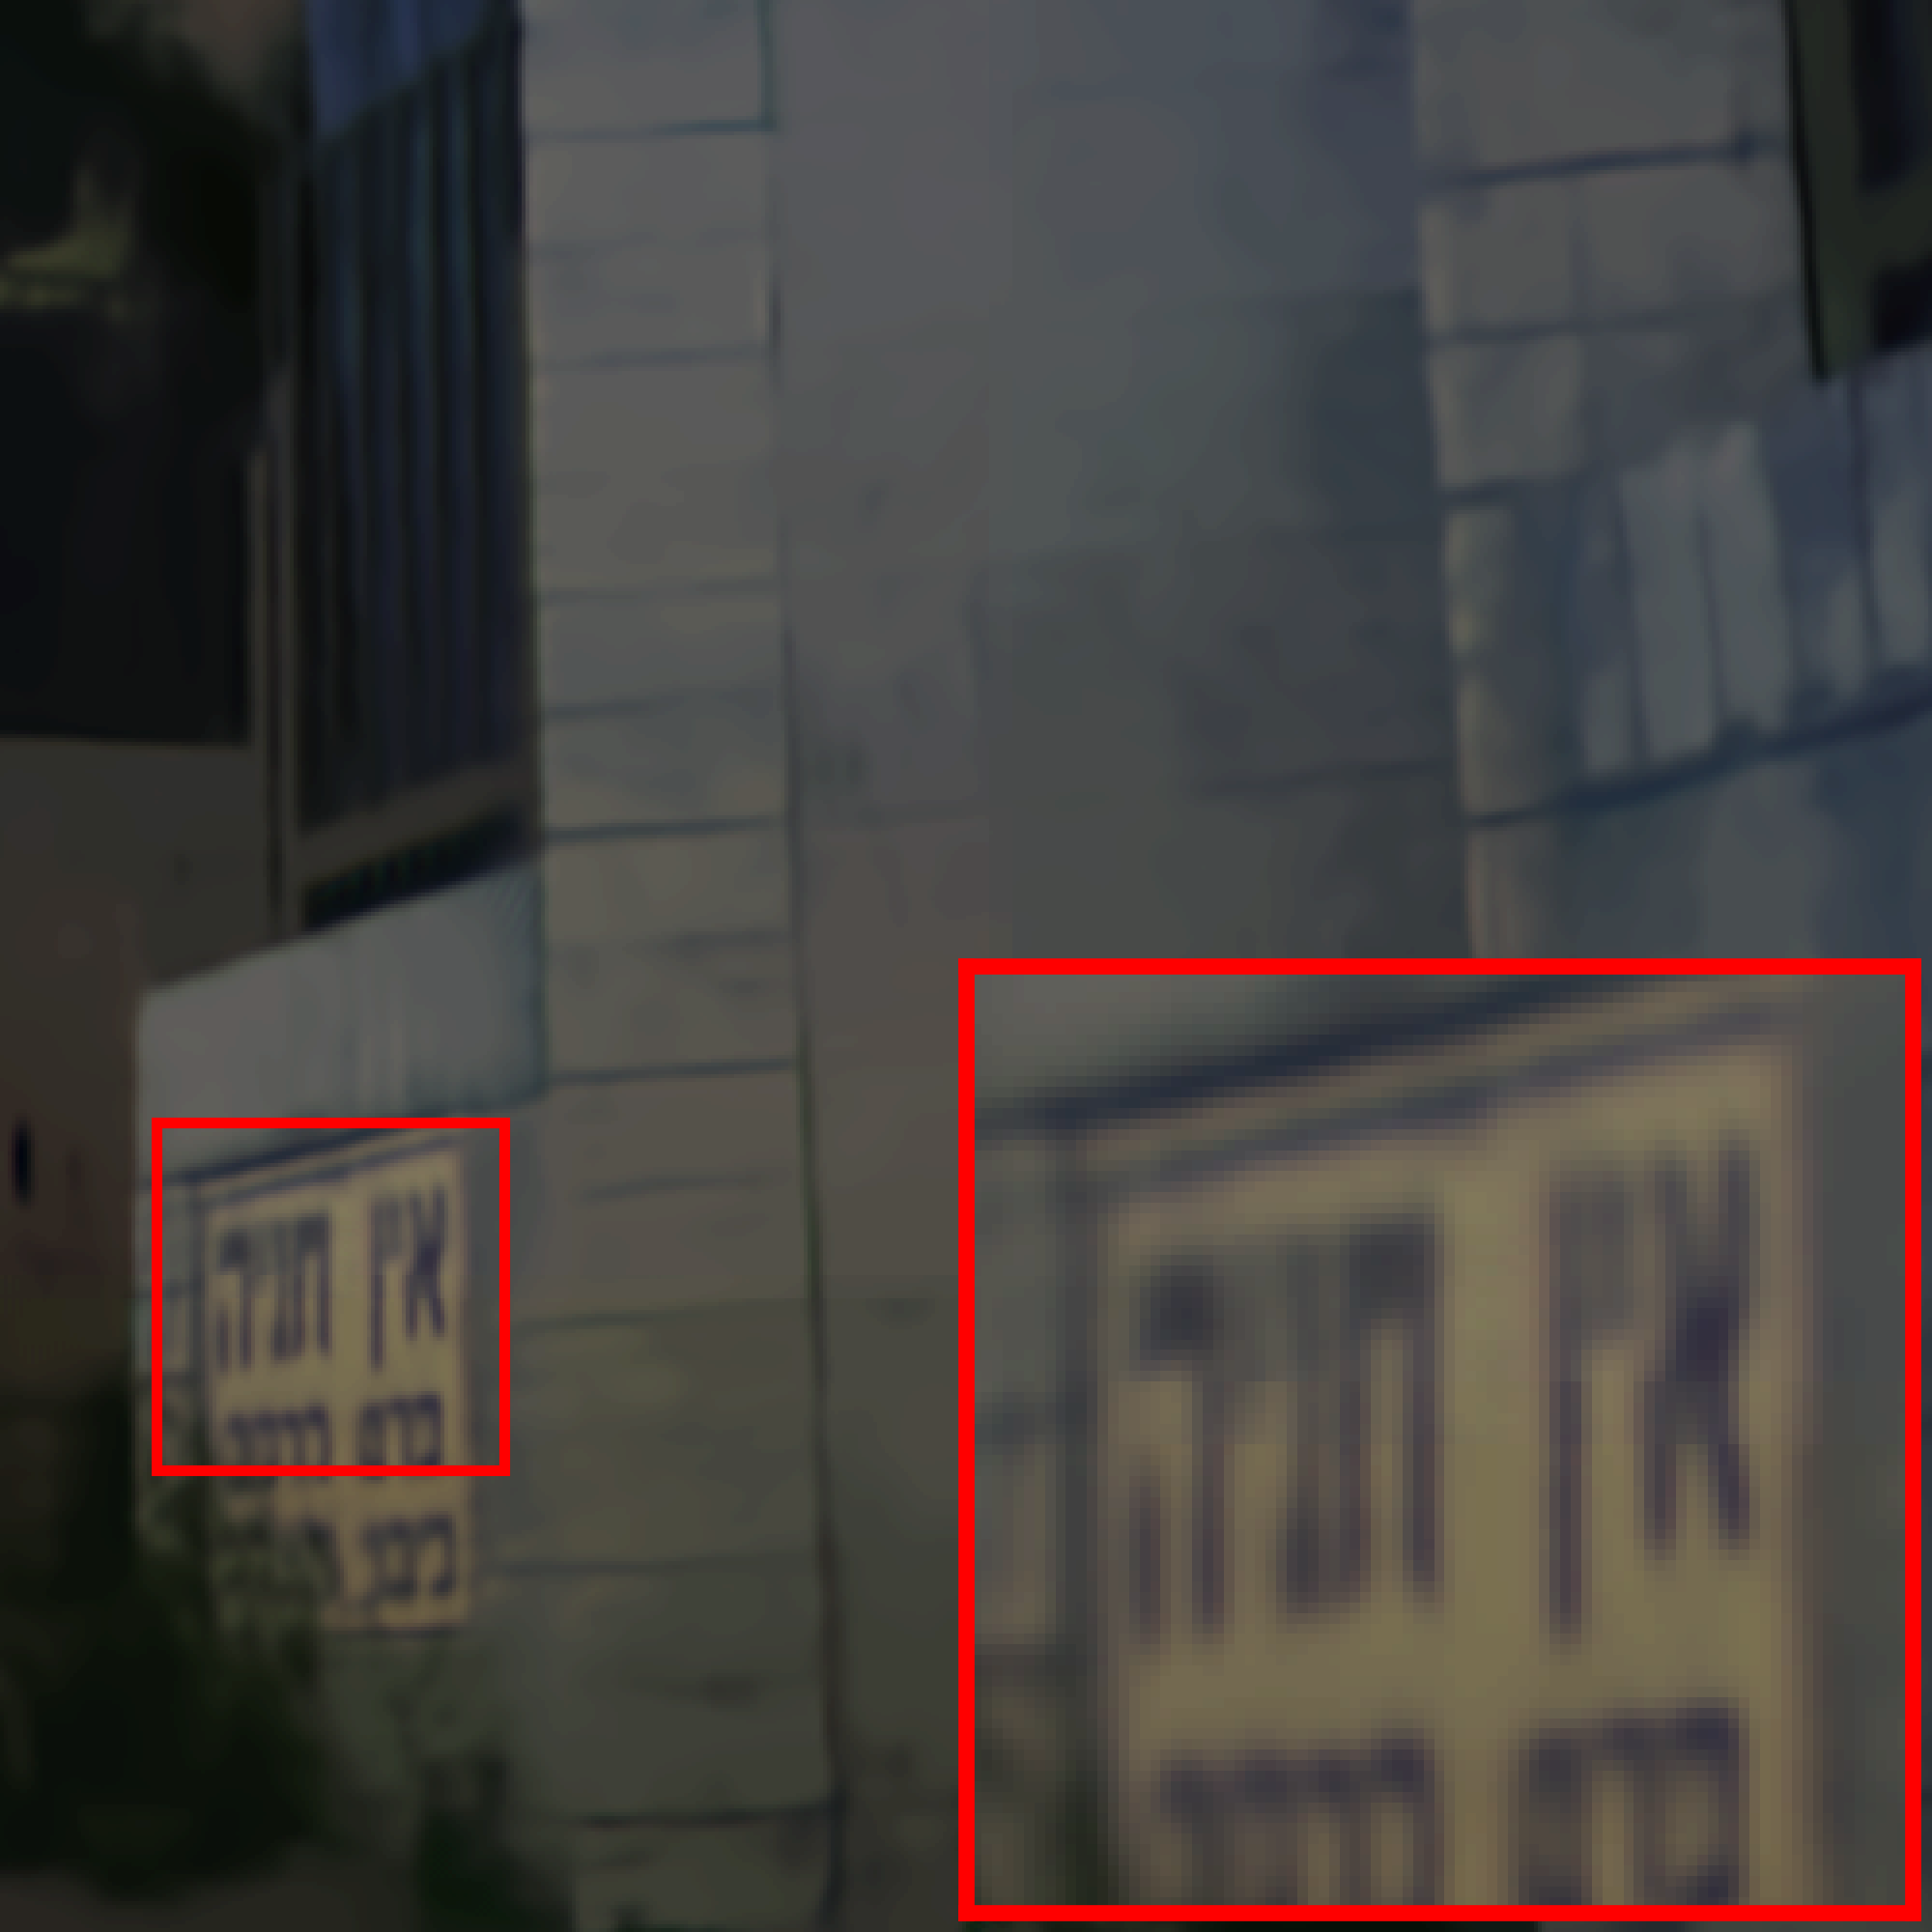
\includegraphics[width=\textwidth]{fichiers_latex/Chap1/figs/icvl_25/llrt.png}};
      \end{tikzpicture}
   \caption{LLRT}
\end{subfigure}
\hfill
\begin{subfigure}[b]{\figscale\textwidth}
      \begin{tikzpicture}[scale=\figscale]
        \node[anchor=south east,inner sep=0] at (0,0) {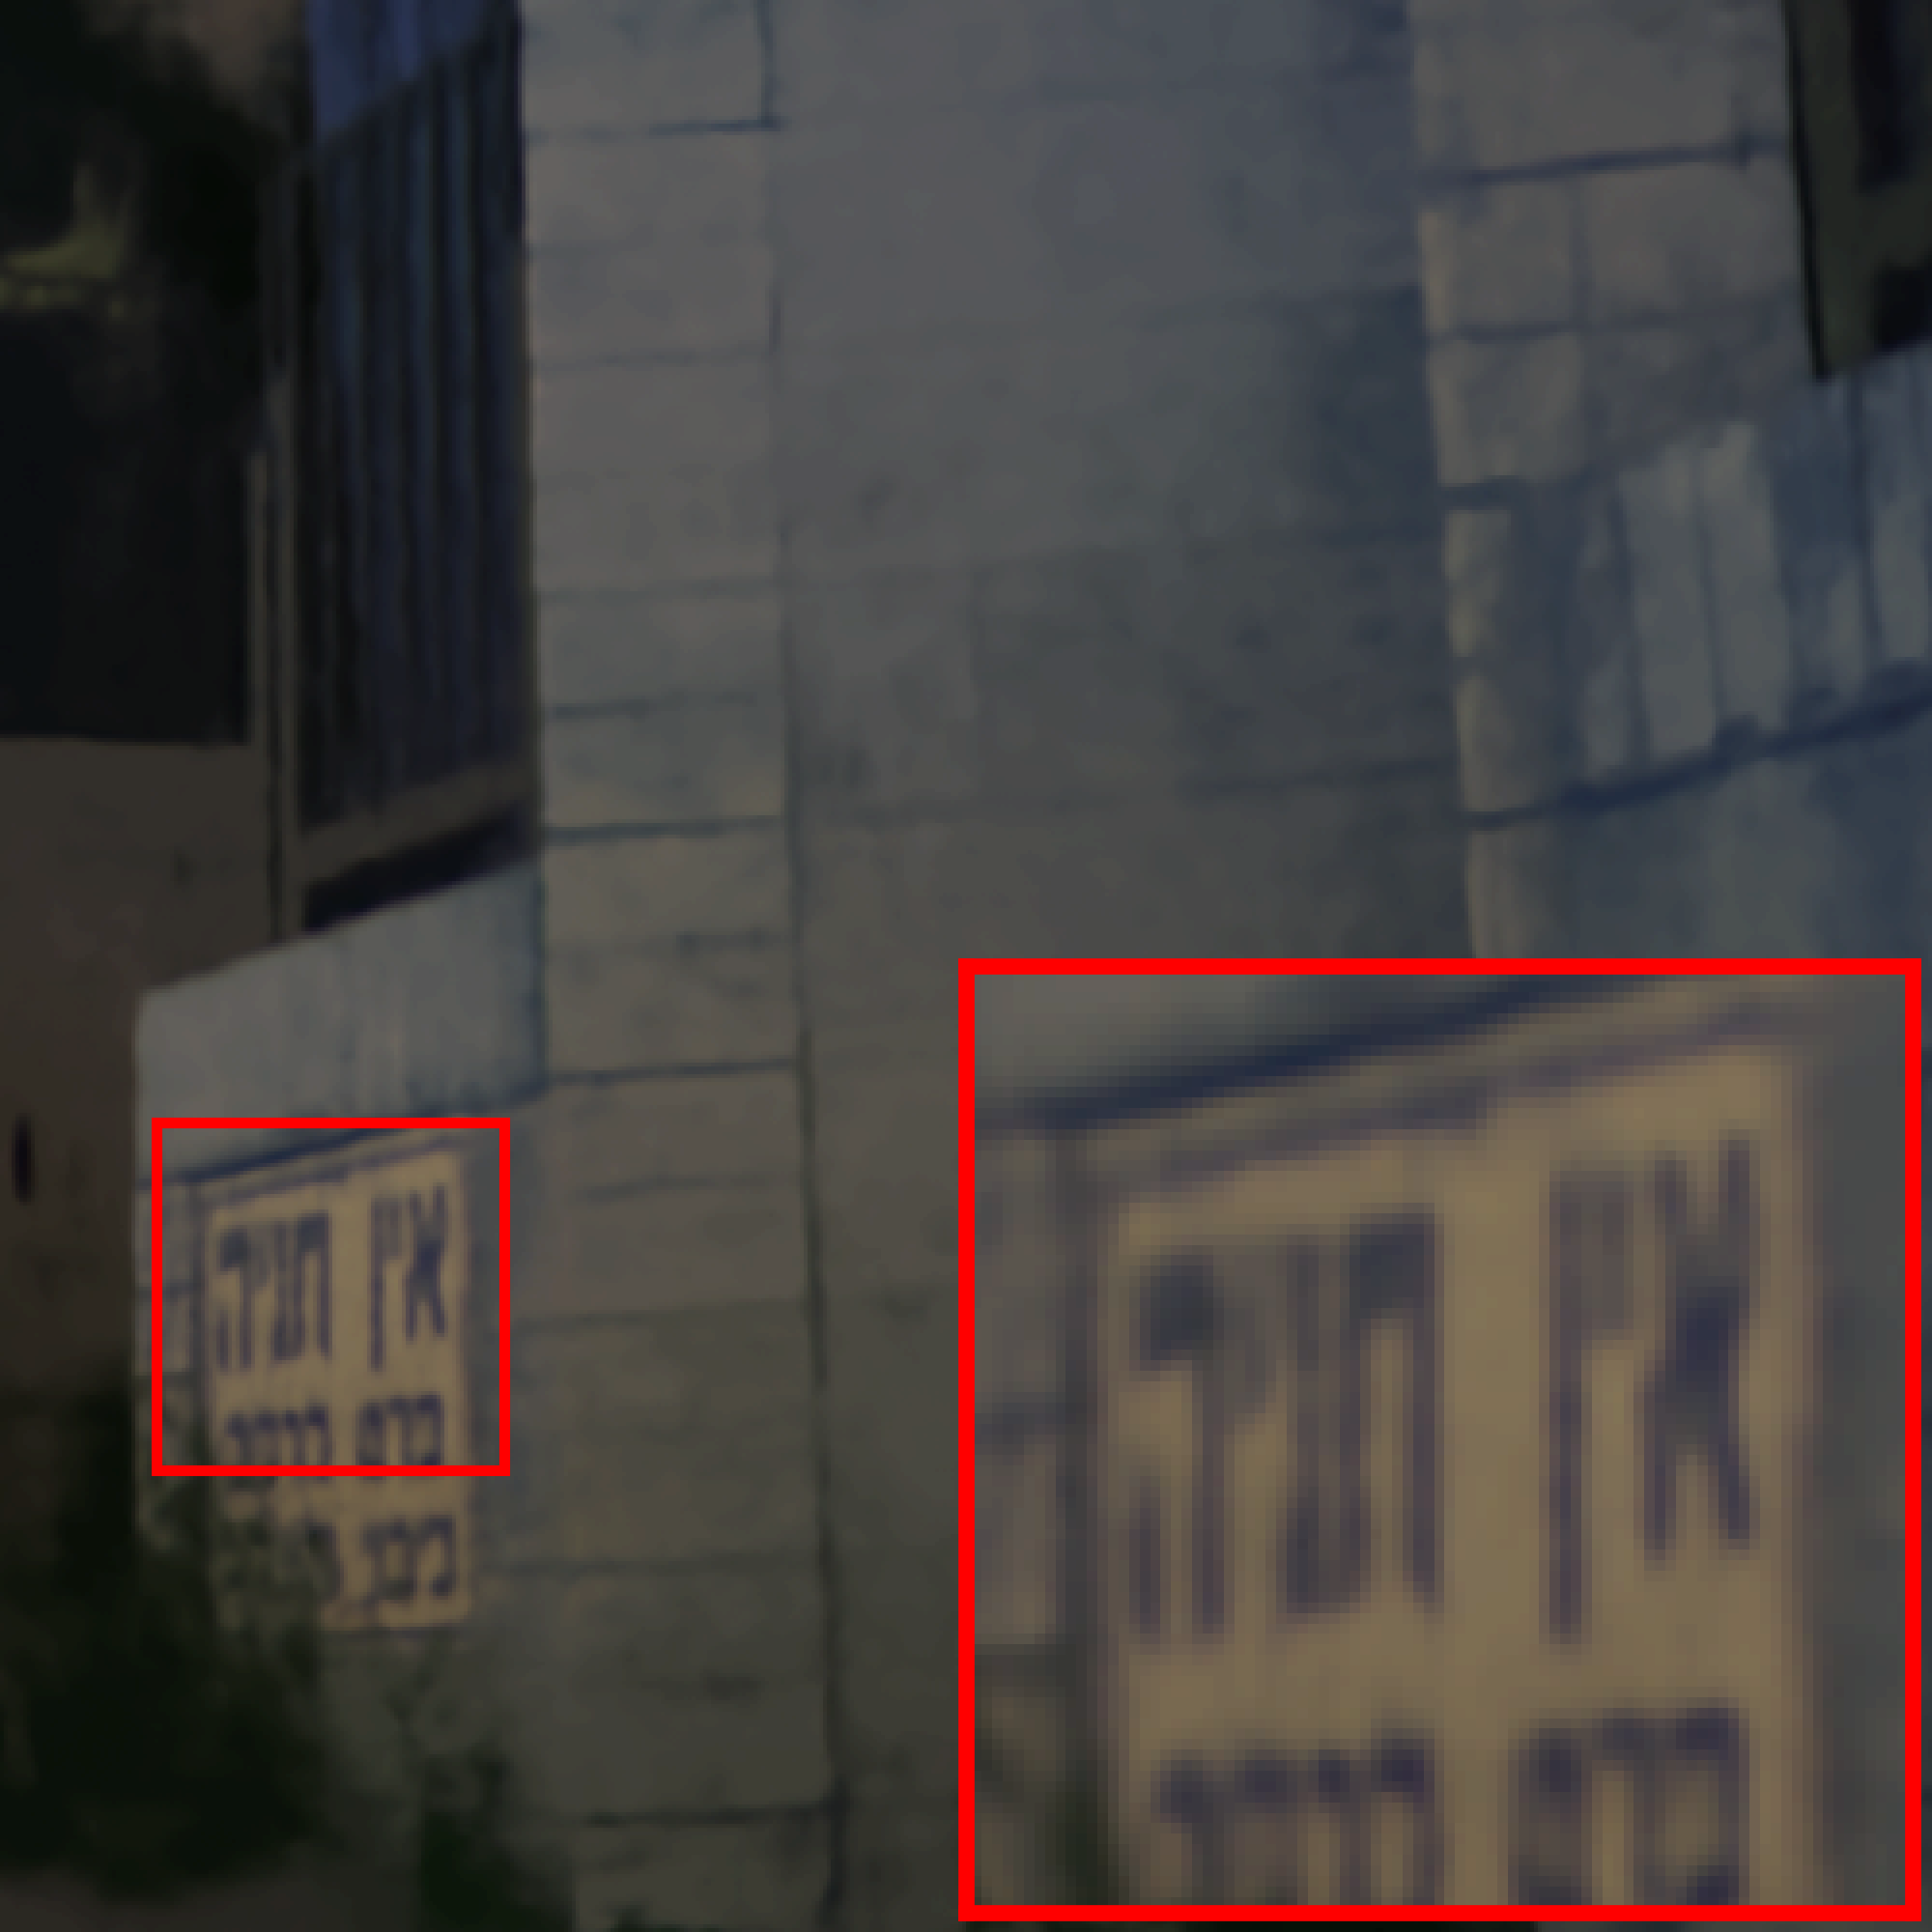
\includegraphics[width=\textwidth]{fichiers_latex/Chap1/figs/icvl_25/ngmeet.png}};
      \end{tikzpicture}
   \caption{NGMeet}
\end{subfigure}
\\
\begin{subfigure}[b]{\figscale\textwidth}
      \begin{tikzpicture}[scale=\figscale]
        \node[anchor=south east,inner sep=0] at (0,0) {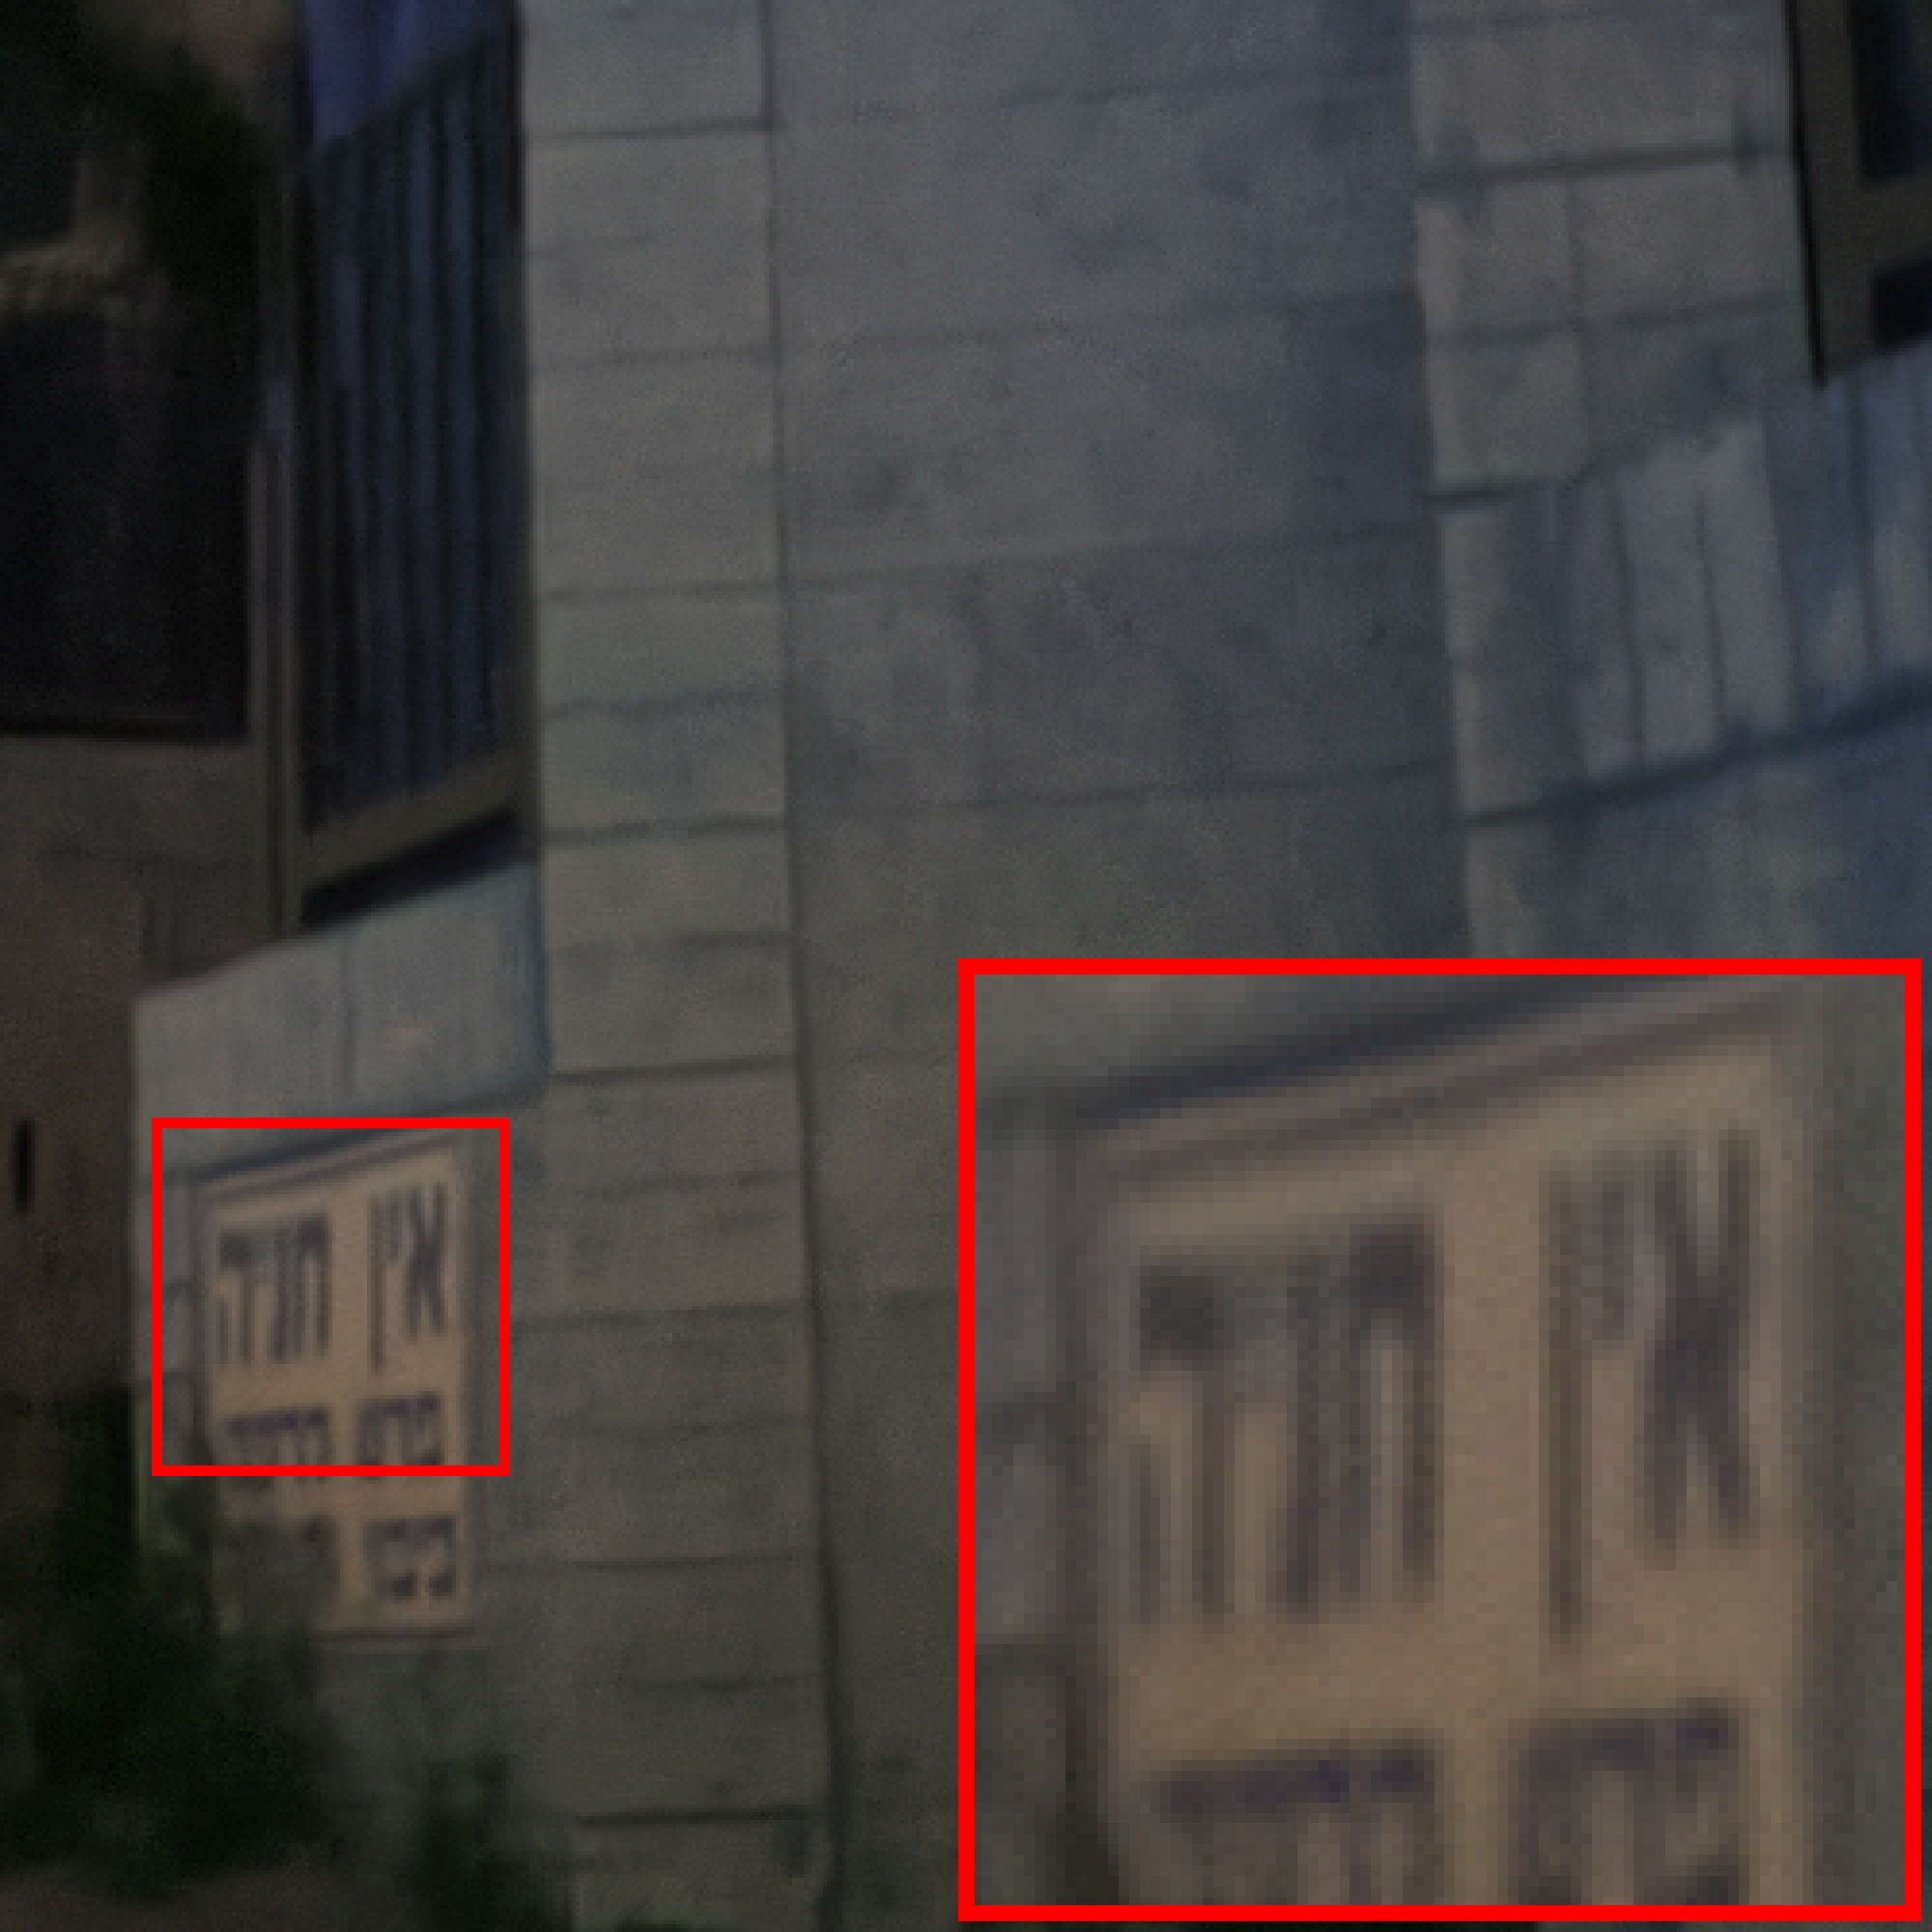
\includegraphics[width=\textwidth]{fichiers_latex/Chap1/figs/icvl_25/glf.png}};
      \end{tikzpicture}
   \caption{GLF}
\end{subfigure} 
\hfill
\begin{subfigure}[b]{\figscale\textwidth}
      \begin{tikzpicture}[scale=\figscale]
        \node[anchor=south east,inner sep=0] at (0,0) {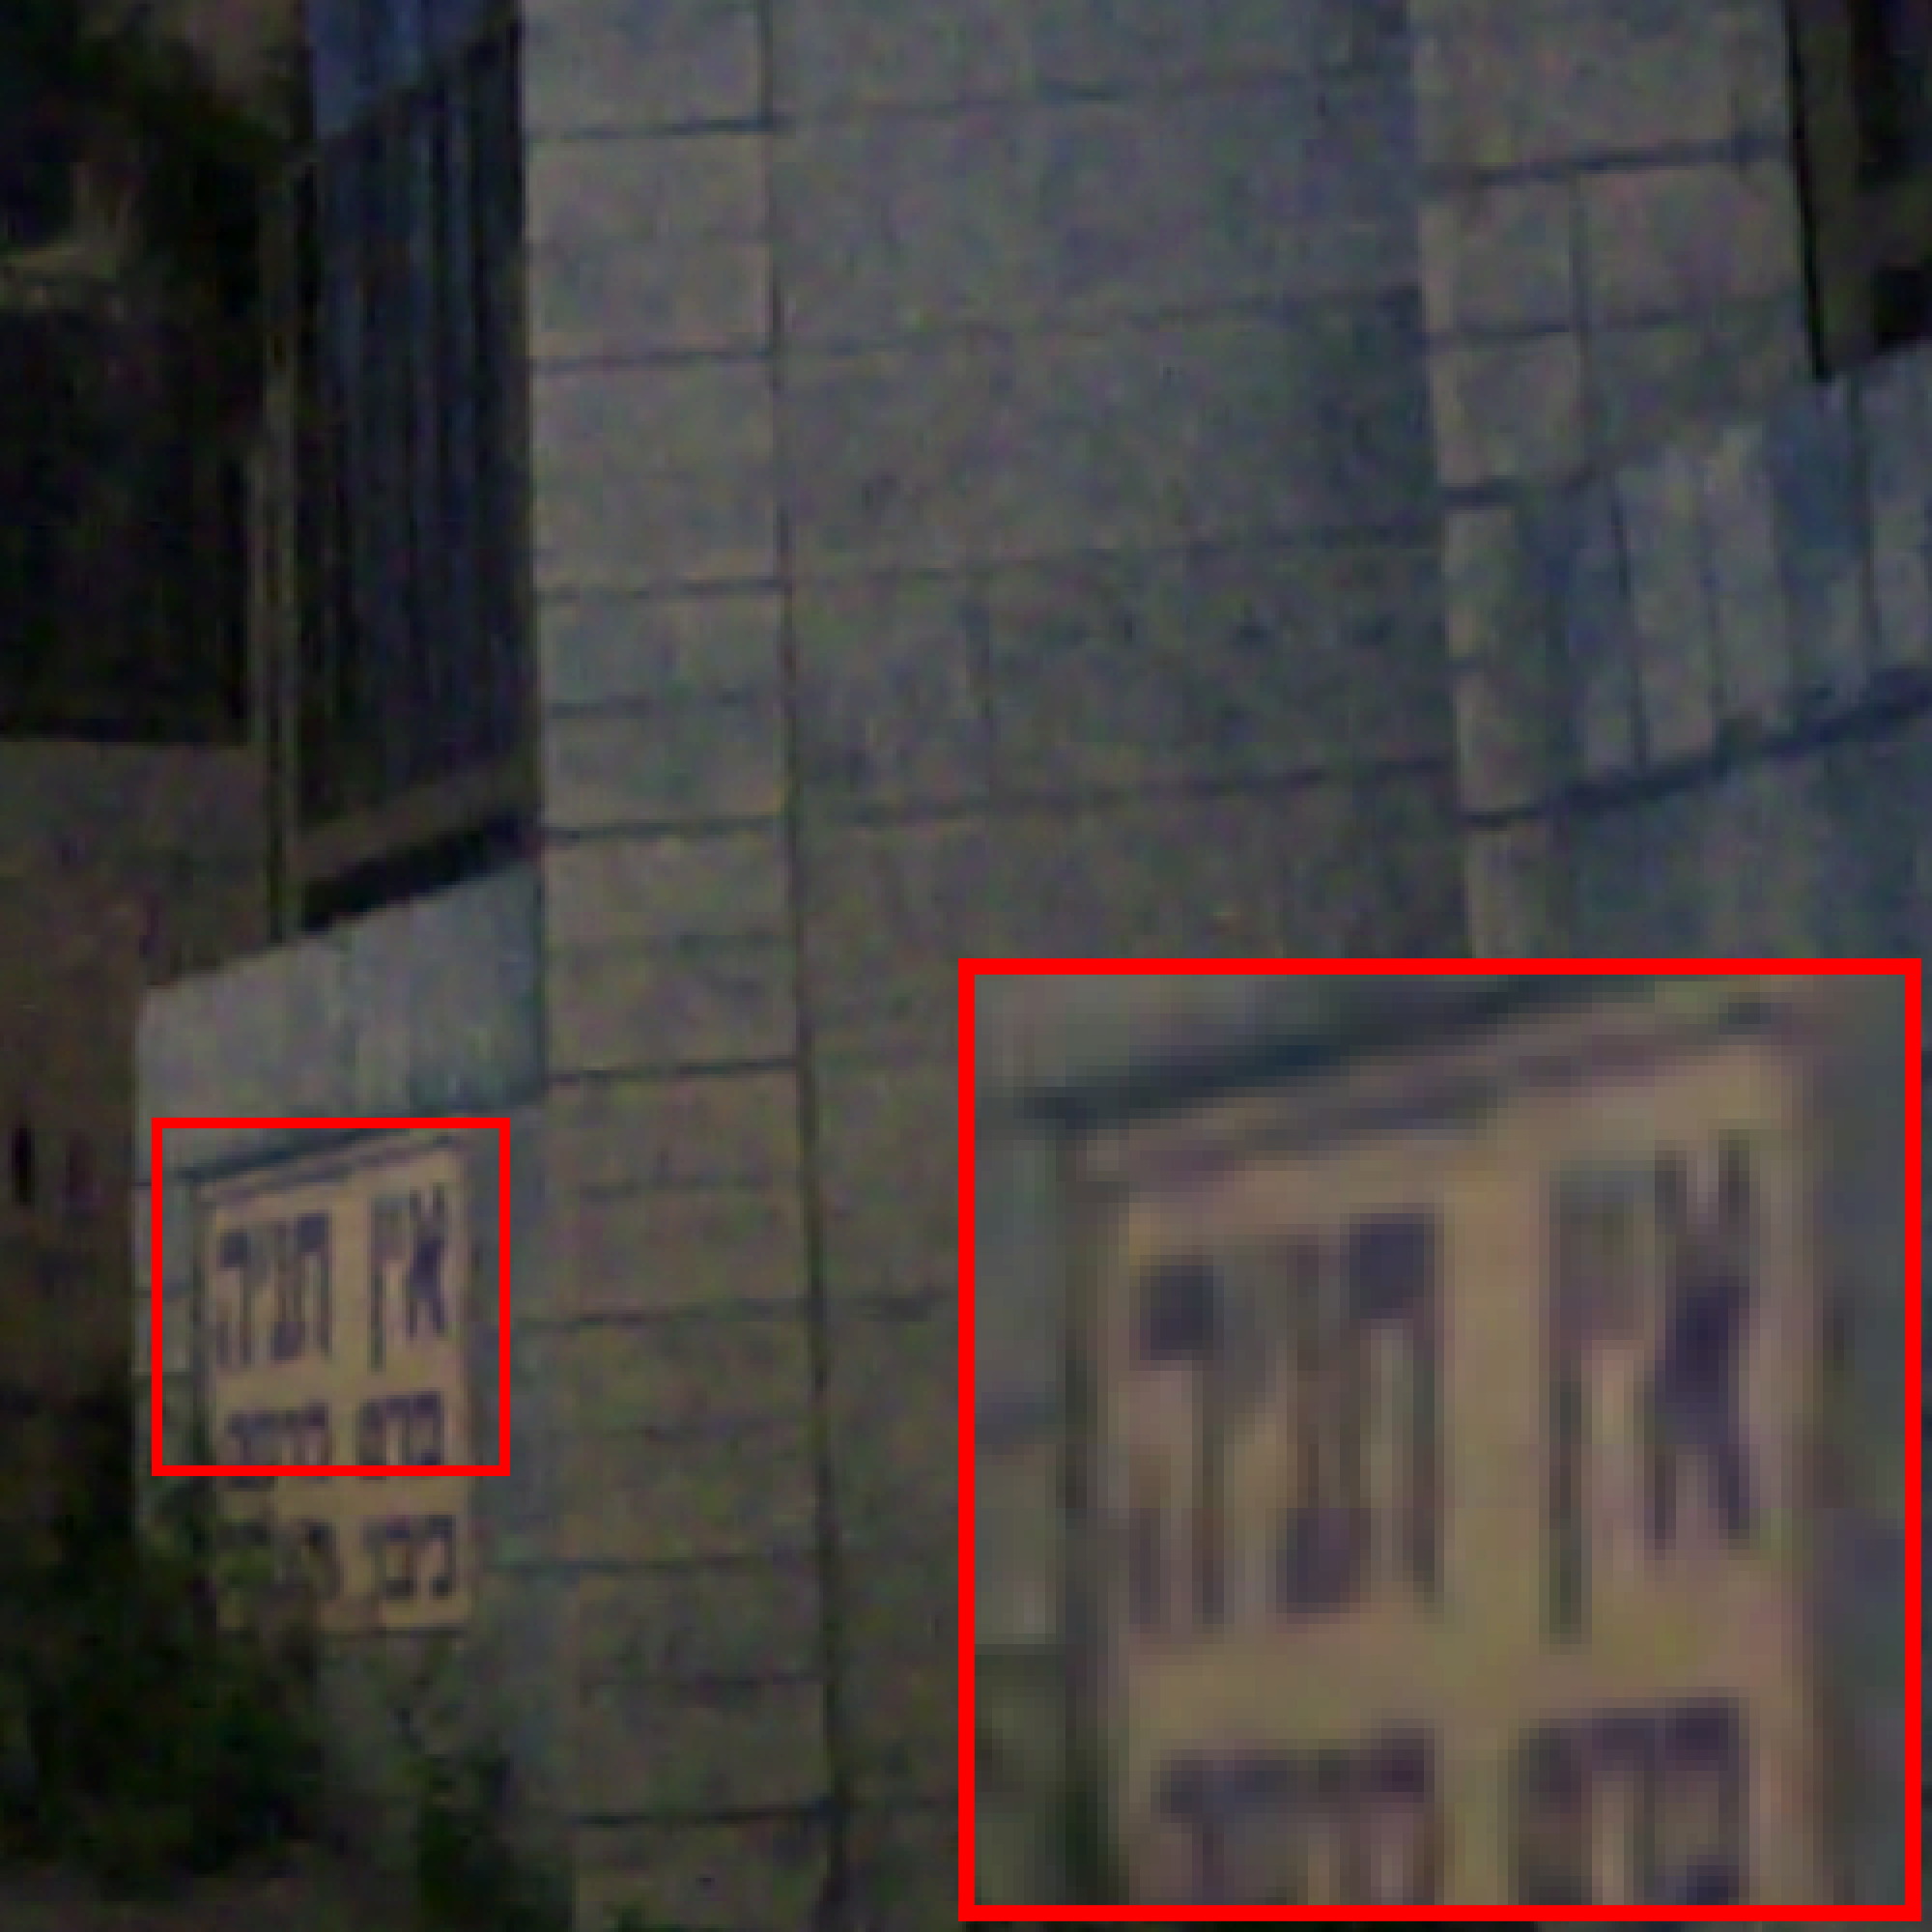
\includegraphics[width=\textwidth]{fichiers_latex/Chap1/figs/icvl_25/smds.png}};
      \end{tikzpicture}
   \caption{SMDS-Net}
\end{subfigure}
\hfill
\begin{subfigure}[b]{\figscale\textwidth}
      \begin{tikzpicture}[scale=\figscale]
        \node[anchor=south east,inner sep=0] at (0,0) {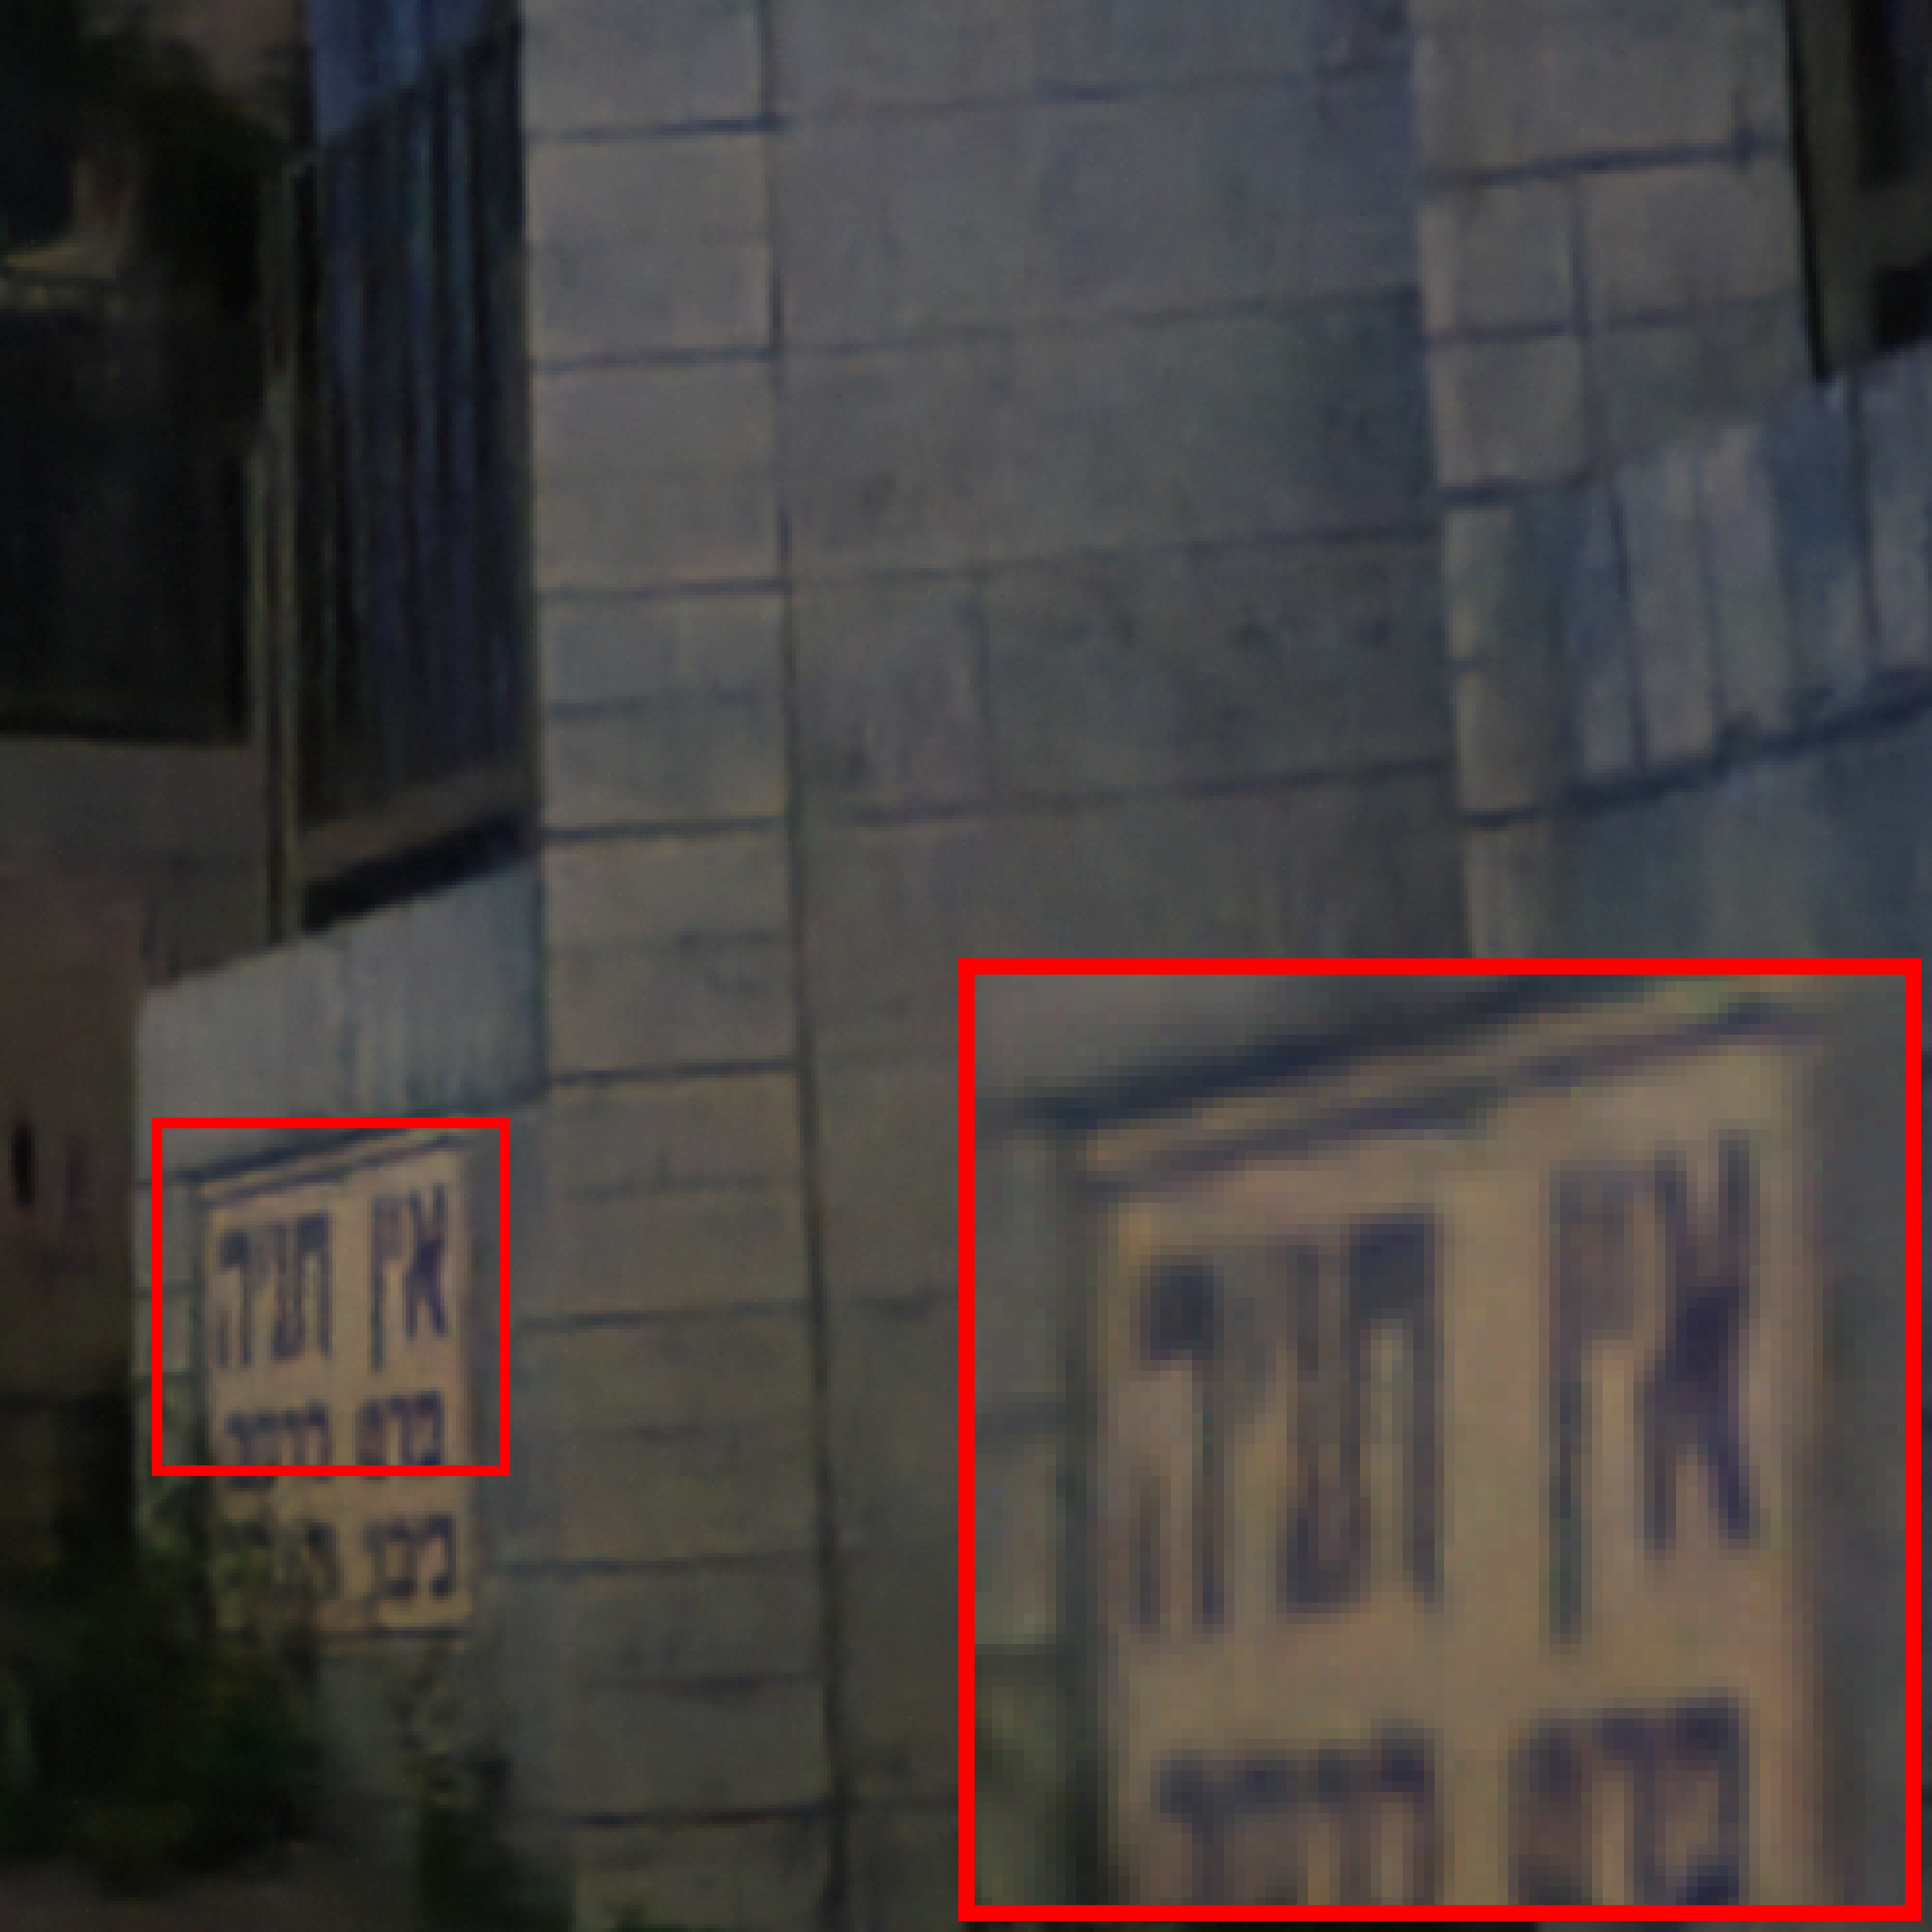
\includegraphics[width=\textwidth]{fichiers_latex/Chap1/figs/icvl_25/qrnn.png}};
      \end{tikzpicture}
   \caption{QRNN3D}
\end{subfigure}
\hfill
\begin{subfigure}[b]{\figscale\textwidth}
      \begin{tikzpicture}[scale=\figscale]
        \node[anchor=south east,inner sep=0] at (0,0) {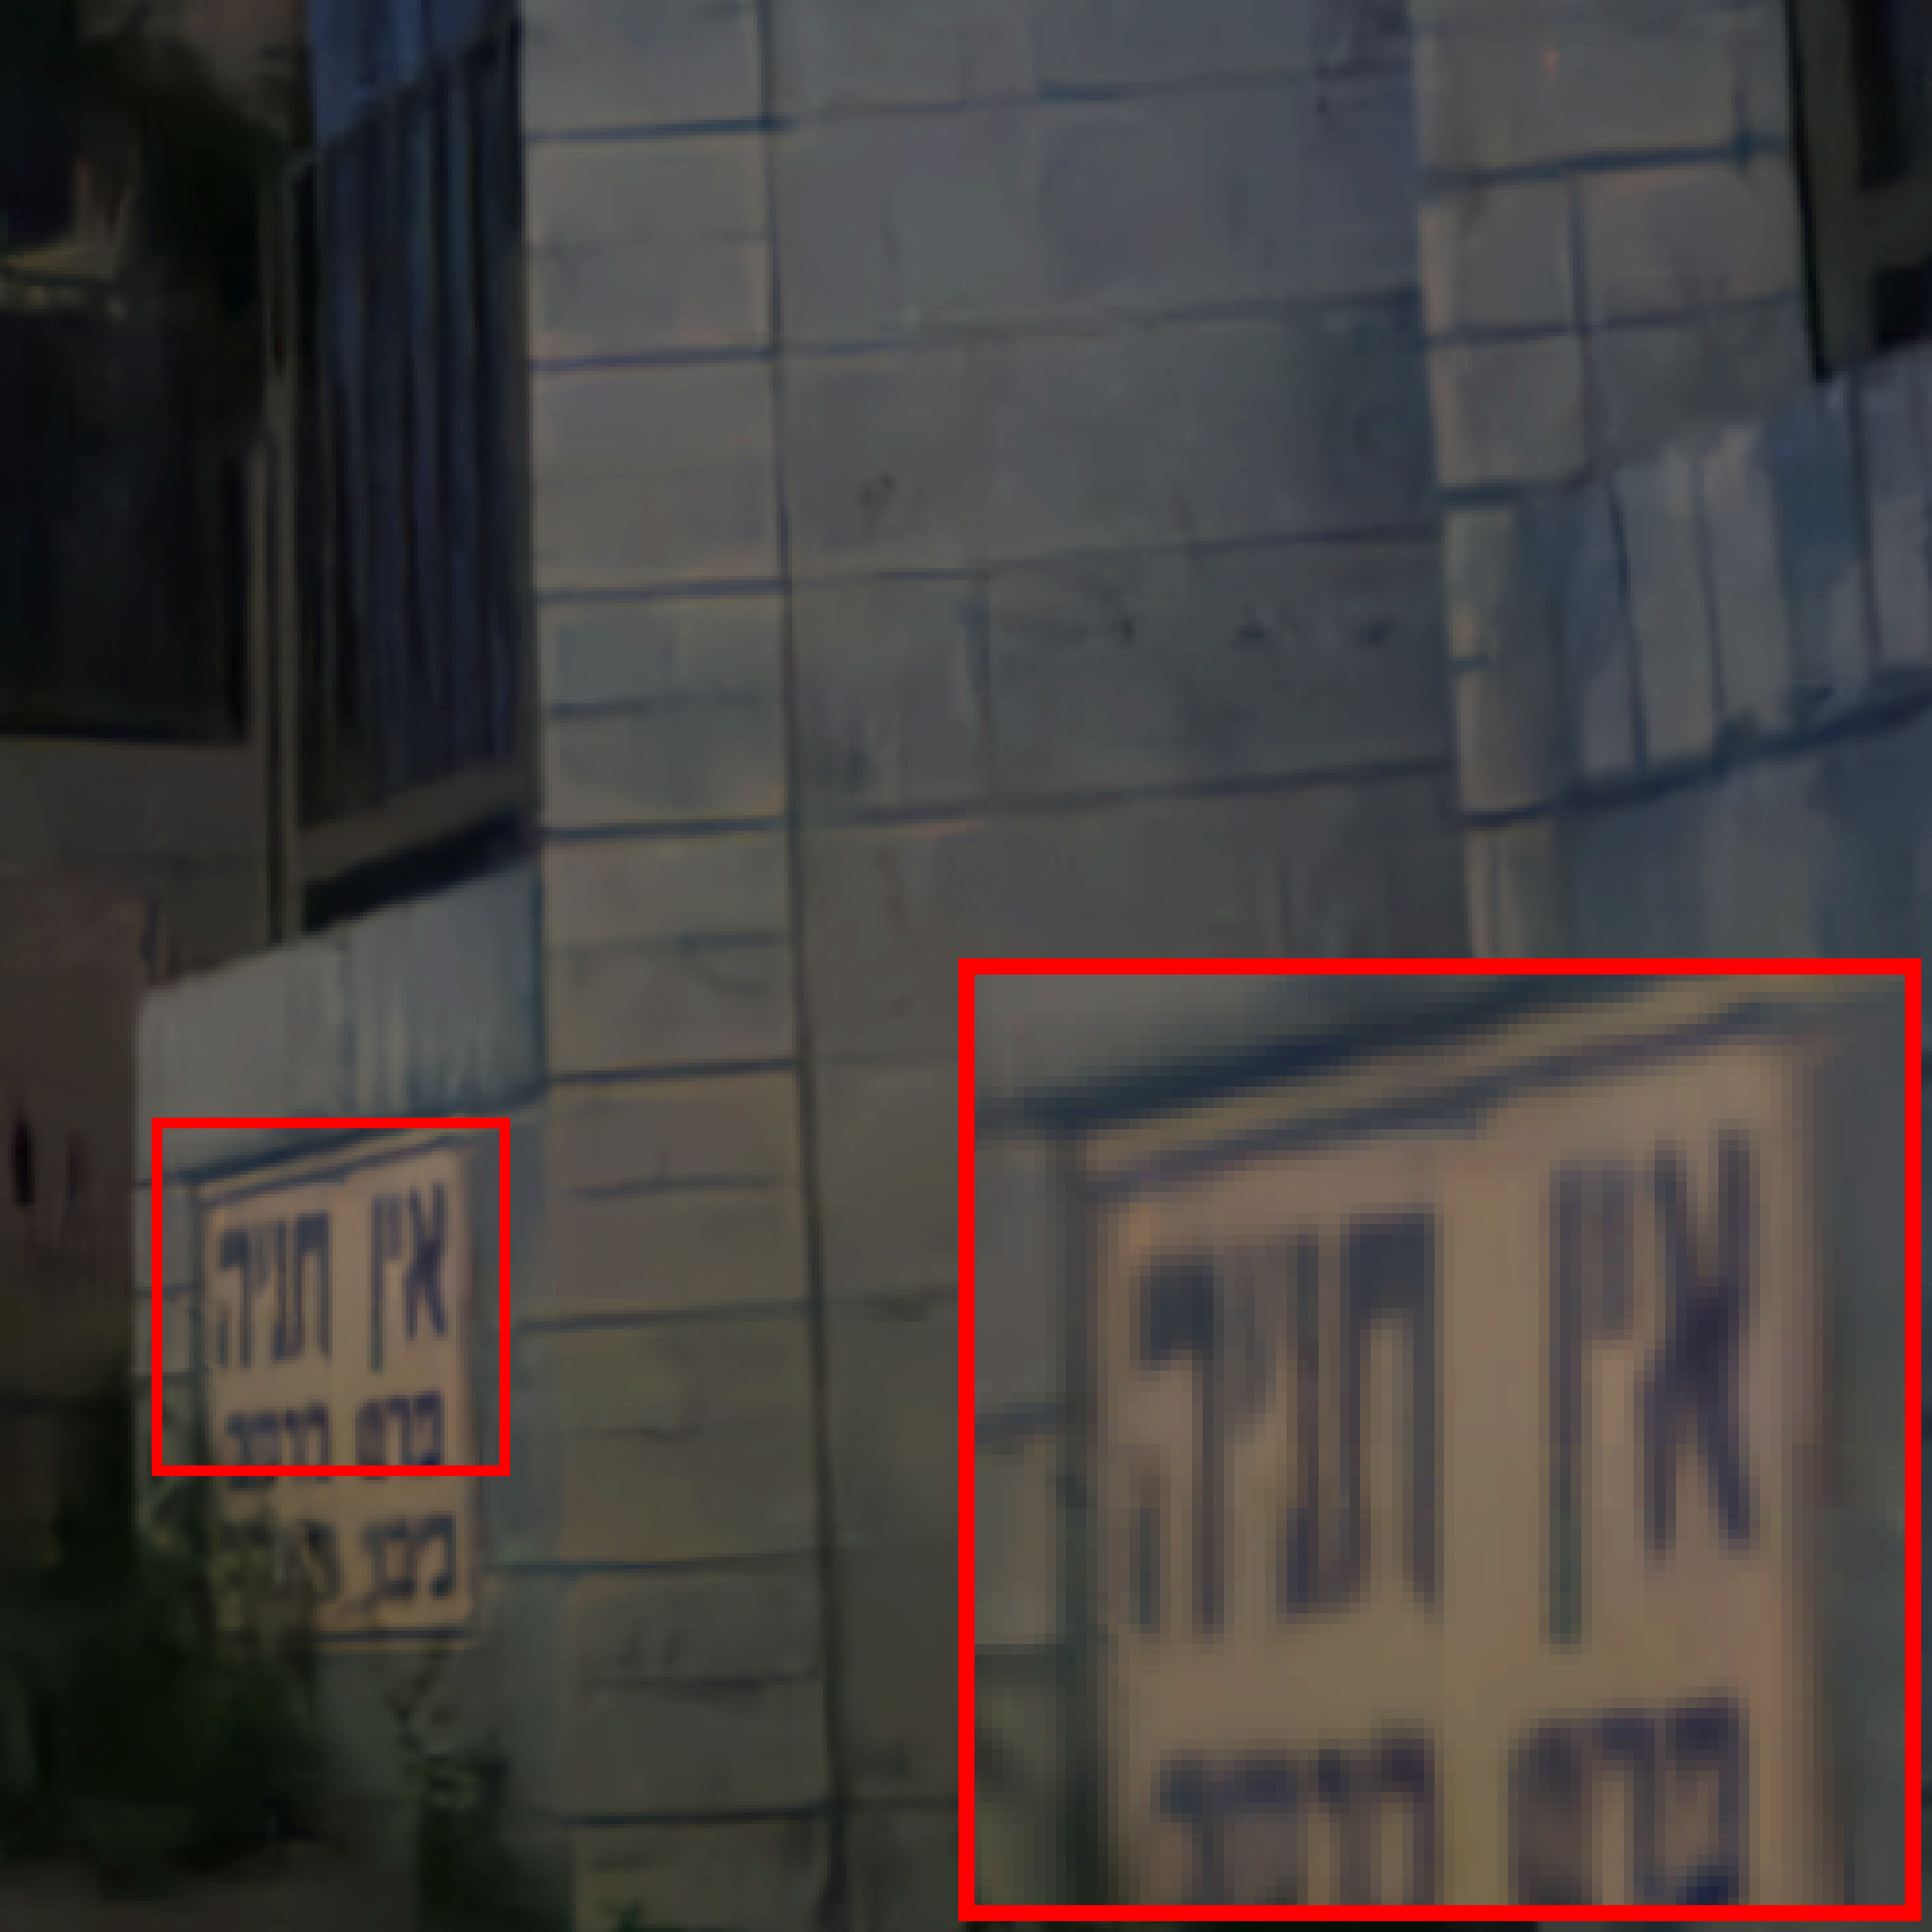
\includegraphics[width=\textwidth]{fichiers_latex/Chap1/figs/icvl_25/t3sc.png}};
      \end{tikzpicture}
   \caption{T3SC}
\end{subfigure}


        \caption{Denoising results with Gaussian noise $\sigma=25$ on ICVL with bands 9, 15, 28.}\label{fig:icvl}
\end{figure}

\begin{figure}[h!]
  
\newcommand{\figscale}{0.24}

\hfill
\begin{subfigure}[b]{\figscale\textwidth}
      \begin{tikzpicture}[scale=\figscale]
        \node[anchor=south east,inner sep=0] at (0,0) {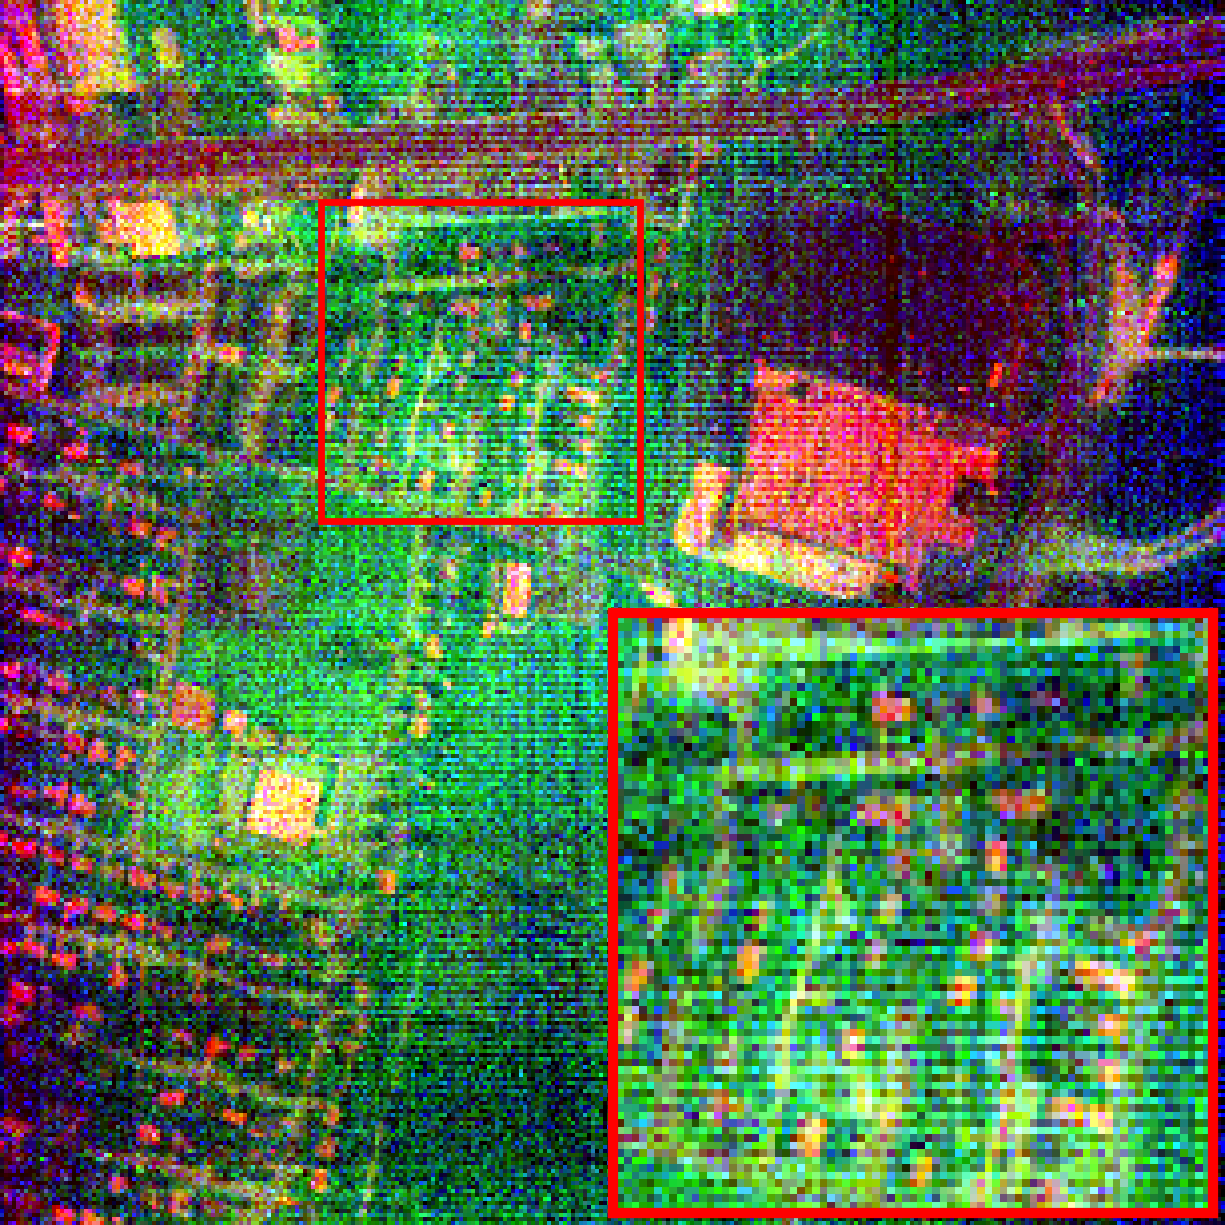
\includegraphics[width=\textwidth]{fichiers_latex/Chap1/figs/urban/in.png}};
      \end{tikzpicture}
   \caption{Input}
\end{subfigure}
\hfill
\begin{subfigure}[b]{\figscale\textwidth}
      \begin{tikzpicture}[scale=\figscale]
        \node[anchor=south east,inner sep=0] at (0,0) {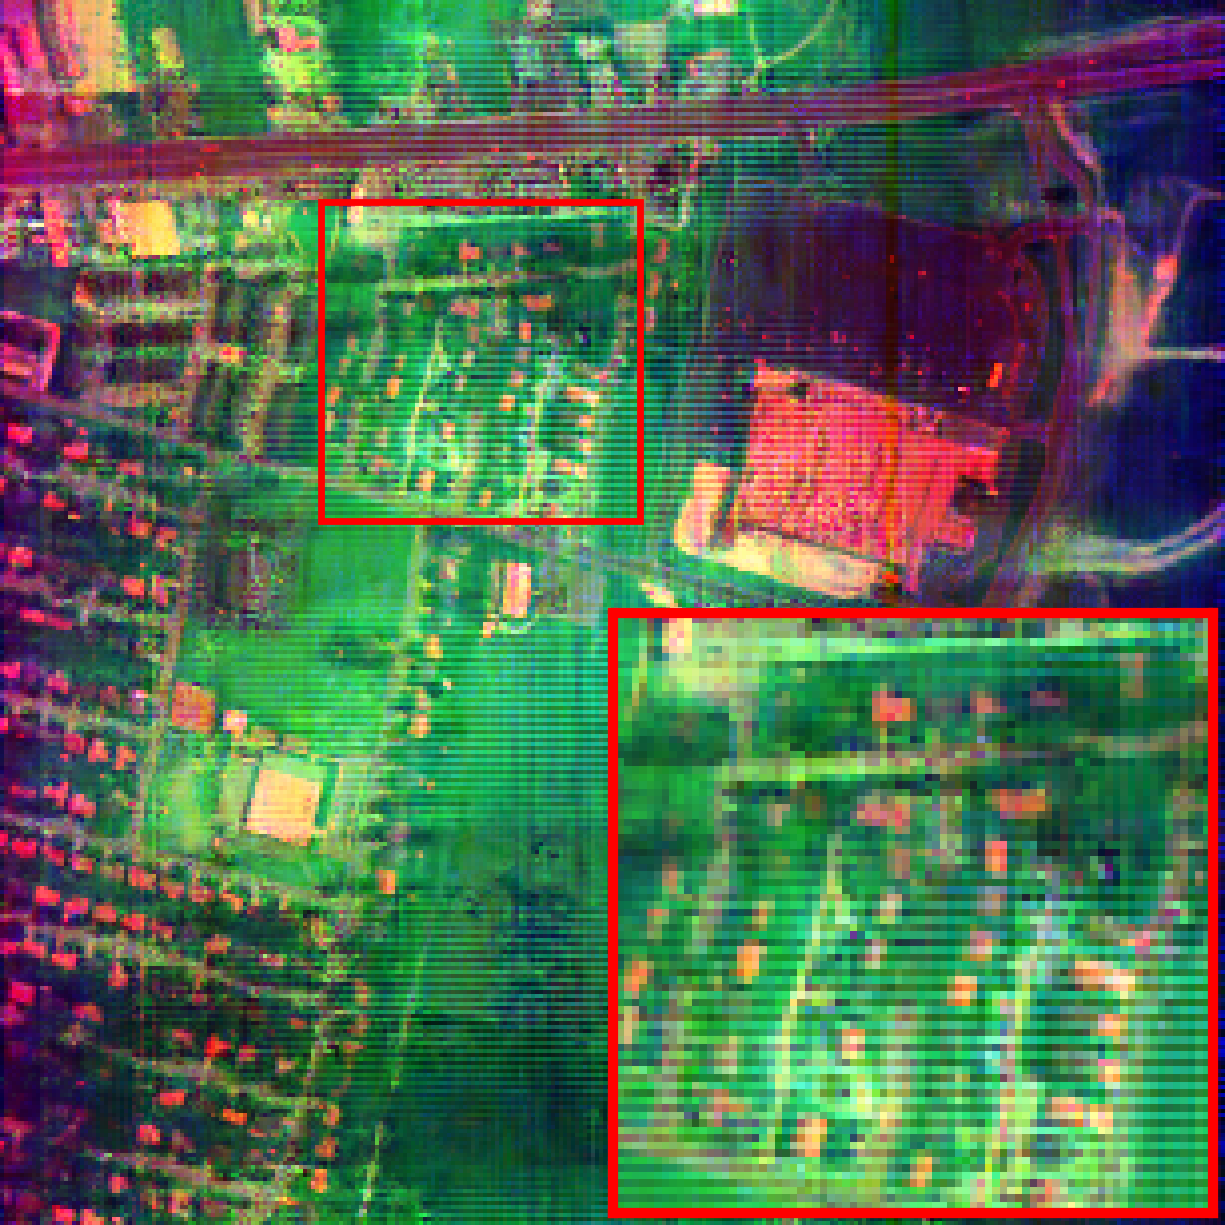
\includegraphics[width=\textwidth]{fichiers_latex/Chap1/figs/urban/bm4d.png}};
      \end{tikzpicture}
   \caption{BM4D}
\end{subfigure}
\hfill
\begin{subfigure}[b]{\figscale\textwidth}
      \begin{tikzpicture}[scale=\figscale]
        \node[anchor=south east,inner sep=0] at (0,0) {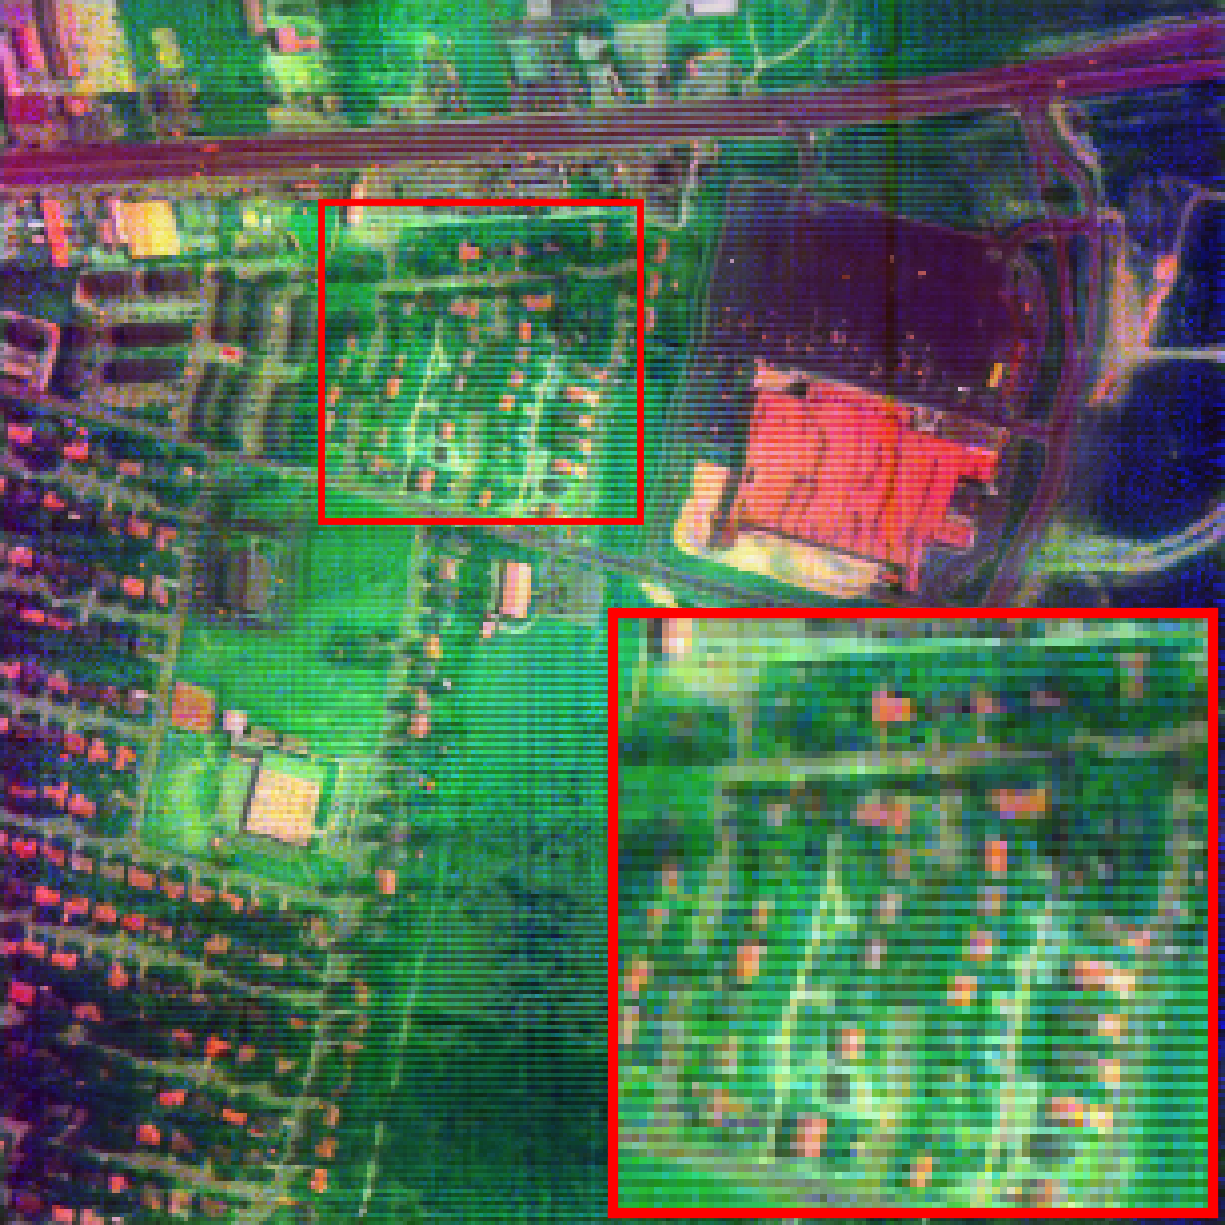
\includegraphics[width=\textwidth]{fichiers_latex/Chap1/figs/urban/llrt.png}};
      \end{tikzpicture}
   \caption{LLRT}
\end{subfigure}
\hfill
\begin{subfigure}[b]{\figscale\textwidth}
      \begin{tikzpicture}[scale=\figscale]
        \node[anchor=south east,inner sep=0] at (0,0) {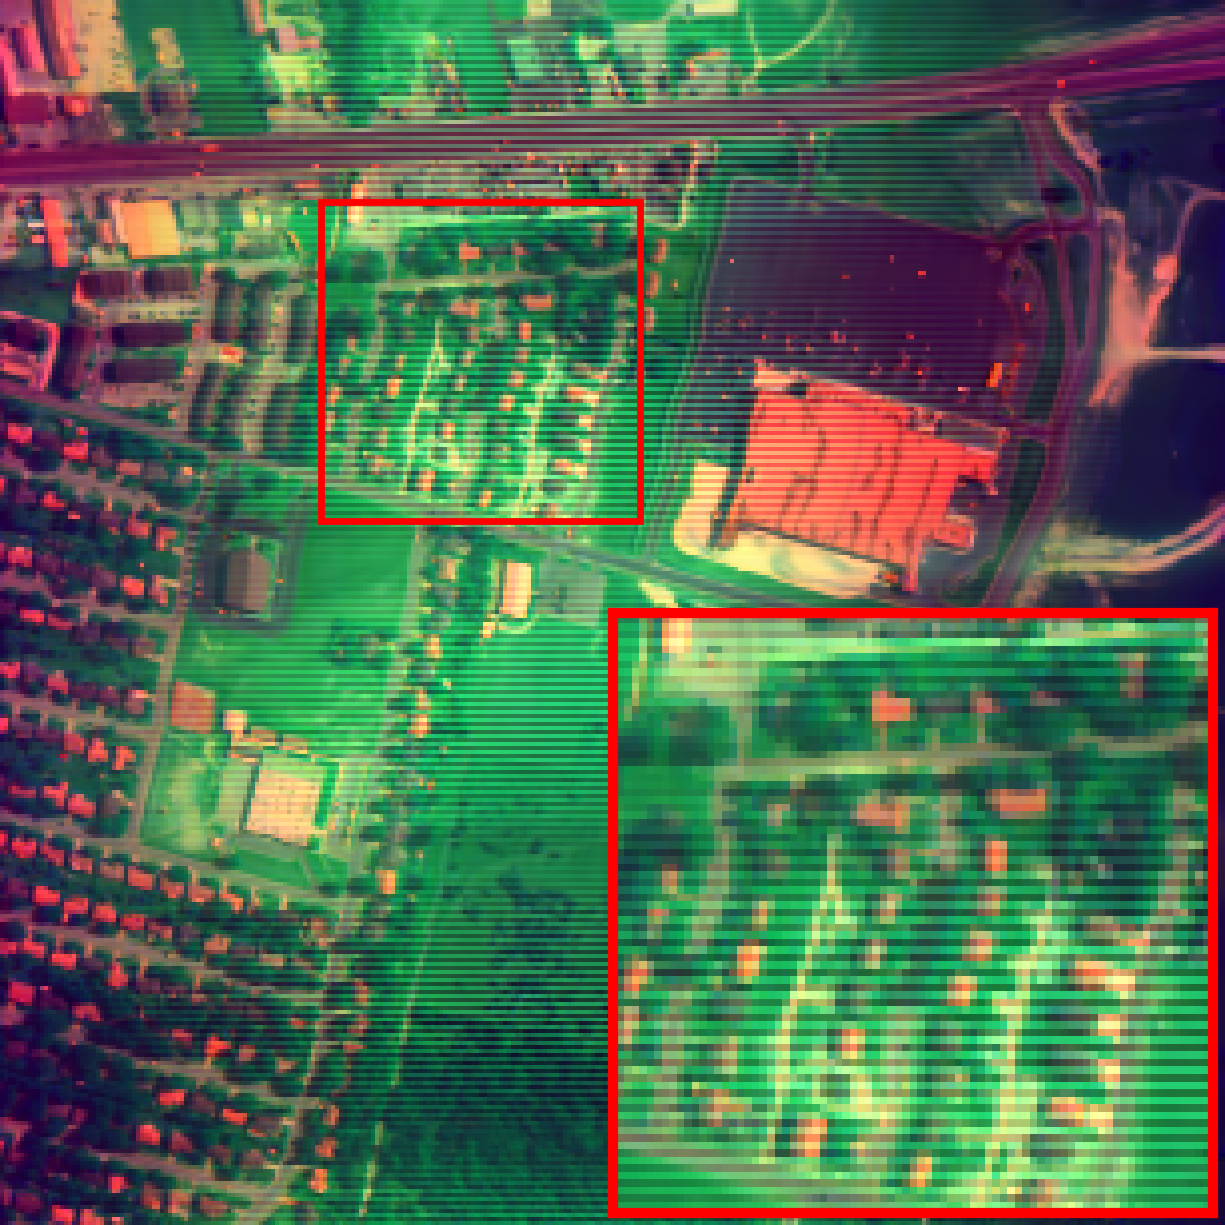
\includegraphics[width=\textwidth]{fichiers_latex/Chap1/figs/urban/ngmeet.png}};
      \end{tikzpicture}
   \caption{NGMeet}
\end{subfigure}
\\
\begin{subfigure}[b]{\figscale\textwidth}
      \begin{tikzpicture}[scale=\figscale]
        \node[anchor=south east,inner sep=0] at (0,0) {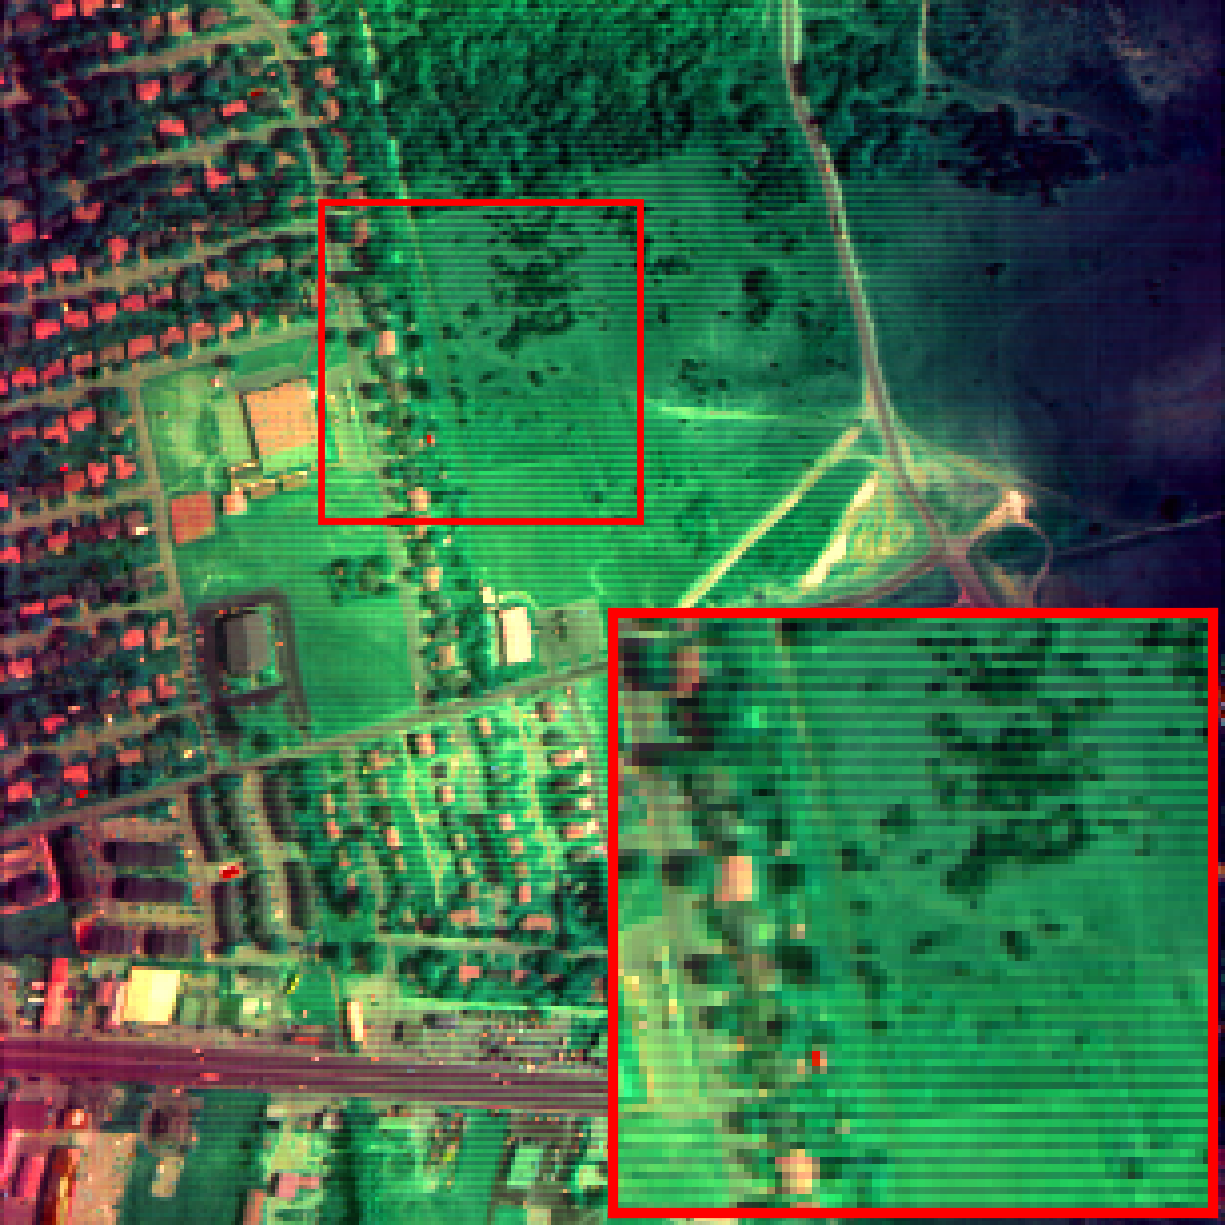
\includegraphics[width=\textwidth]{fichiers_latex/Chap1/figs/urban/glf.png}};
      \end{tikzpicture}
   \caption{GLF}
\end{subfigure} 
\hfill
\begin{subfigure}[b]{\figscale\textwidth}
      \begin{tikzpicture}[scale=\figscale]
        \node[anchor=south east,inner sep=0] at (0,0) {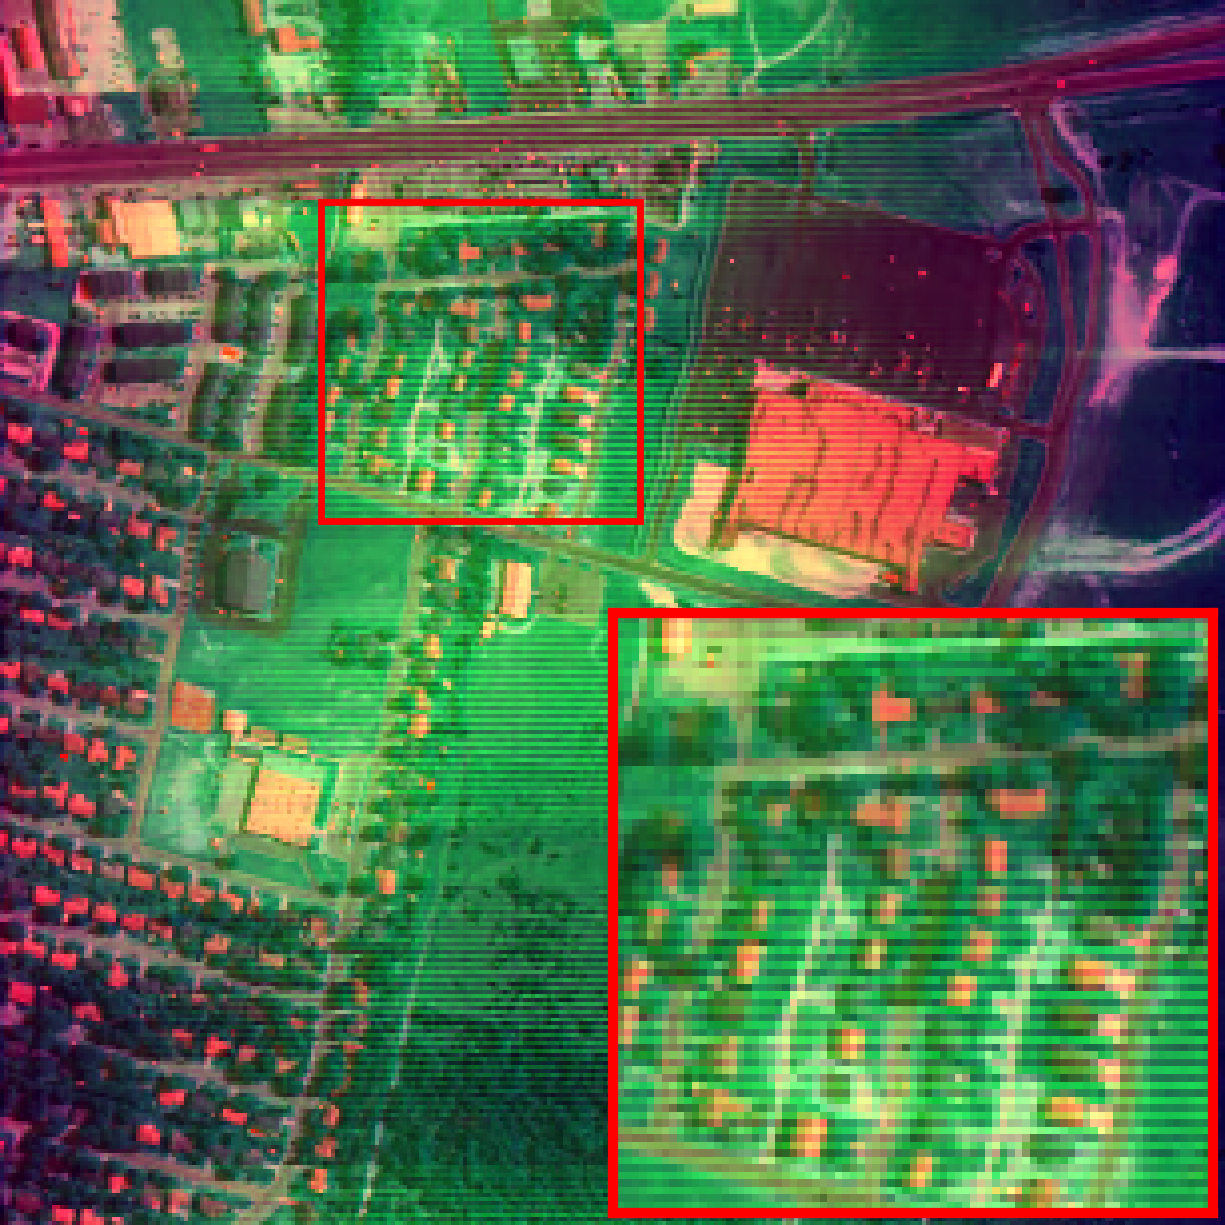
\includegraphics[width=\textwidth]{fichiers_latex/Chap1/figs/urban/smds.png}};
      \end{tikzpicture}
   \caption{SMDS-Net}
\end{subfigure}
\hfill
\begin{subfigure}[b]{\figscale\textwidth}
      \begin{tikzpicture}[scale=\figscale]
        \node[anchor=south east,inner sep=0] at (0,0) {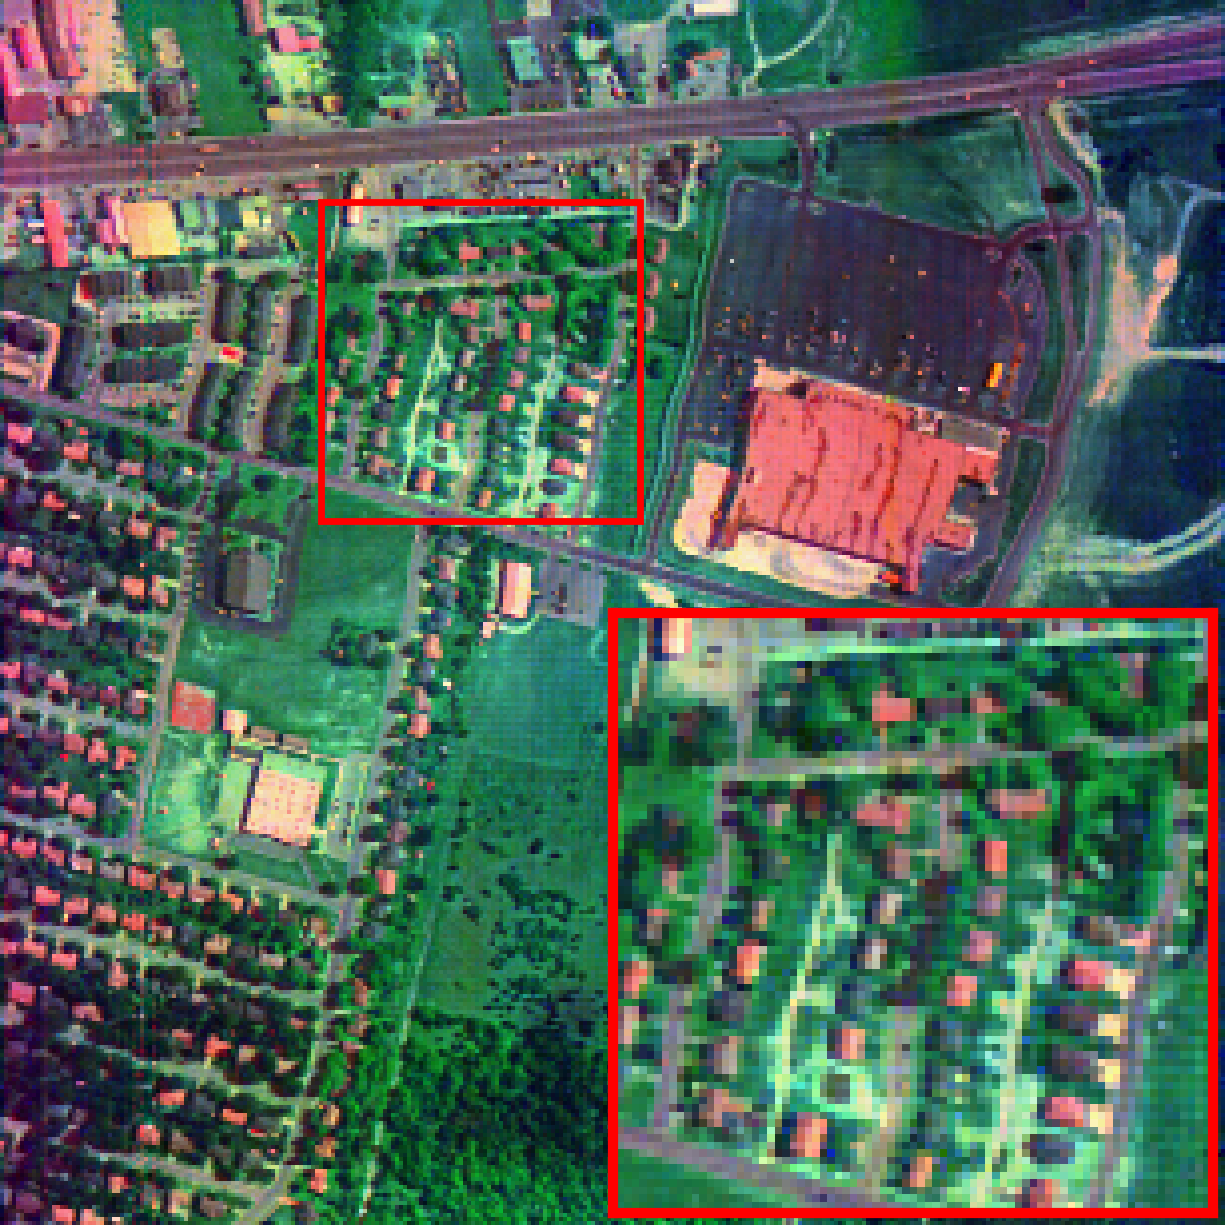
\includegraphics[width=\textwidth]{fichiers_latex/Chap1/figs/urban/qrnn.png}};
      \end{tikzpicture}
   \caption{QRNN3D}
\end{subfigure}
\hfill
\begin{subfigure}[b]{\figscale\textwidth}
      \begin{tikzpicture}[scale=\figscale]
        \node[anchor=south east,inner sep=0] at (0,0) {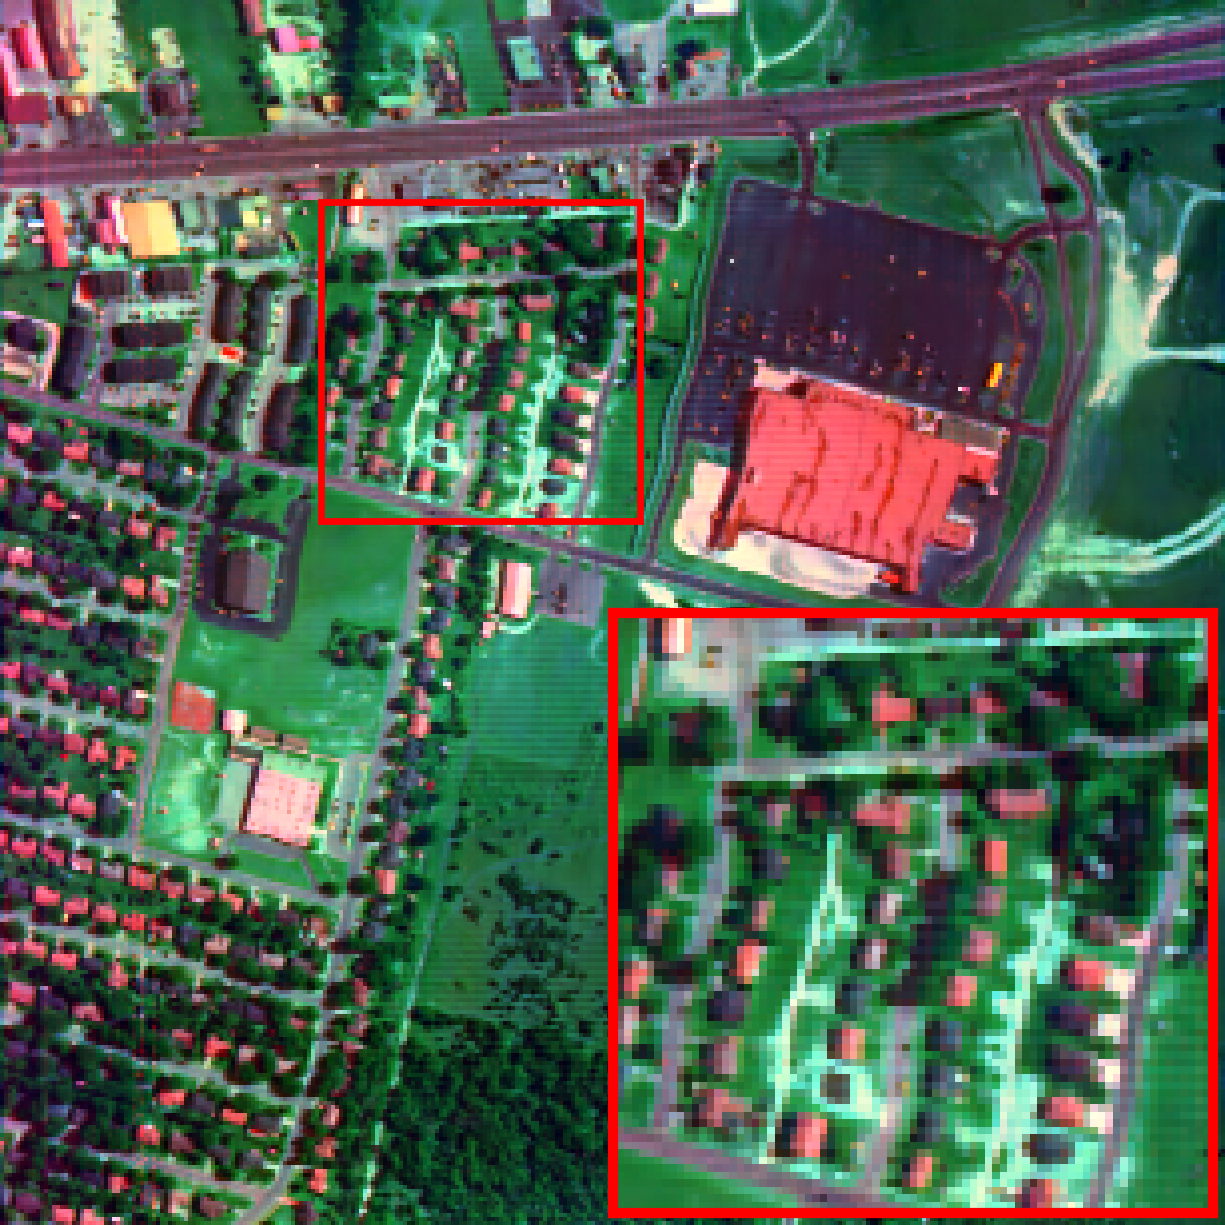
\includegraphics[width=\textwidth]{fichiers_latex/Chap1/figs/urban/t3sc_bs.png}};
      \end{tikzpicture}
   \caption{T3SC}
\end{subfigure}


        \caption{Visual result on a real HSI denoising experiment on Urban dataset with bands 1, 108, 208.}\label{fig:urban}
\end{figure}


\subsubsection{Broader impact}

This chapter addresses the problem of denoising the signal, which is a key pre-processing step before using hyperspectral signals in concrete applications. 
As such, it is necessarily subject to dual use.
For instance, HS imaging may be used for environmental monitoring, forestry, yield estimation in agriculture, natural disaster management planning, astronomy, archaeology, and medicine.
Yet, HS imaging is also used by the petroleum industry for finding new oil fields, and has obvious military applications for surveillance.
We believe the potential benefits of HSI for society are large enough to outweigh the potential harm. 
Nevertheless, we are planning to implement appropriate dissemination strategies to mitigate the risk of misuse for this work (notably with restrictive software licenses), while targeting a gold standard regarding the scientific reproducibility of our results.


\chapter*{Appendix}

\section{Implementation details}

In this section, we provide additional implementation details, which are useful to reproduce our experiments (note that the code is also provided).

\paragraph{Noise with spectrally correlated variance.}
For each band $i \in \{ 0, \ldots, c -1 \}$, the standard deviation of the Gaussian noise is defined as :
$$
\sigma_i = \beta \ exp \left[ - \frac{1}{4 \eta^2} \left(\frac{i}{c} - \frac{1}{2}\right)^2  \right]
$$
with $\beta=23.08$ and $\eta=0.157$.

\paragraph{Preprocessing.}
A basic centering step is used for each input patch of our model.
More precisely, for the first layer, each band of the input hyperspectral image is
centered independently prior to patches extraction, and means are added
back after decoding.
For the second layer, patches are centered independently for each band (and similarly, the means are added back after decoding).

\paragraph{Code and patch sizes}
The hyperparameters of our model are presented in Table~\ref{table:model_arch}.

\begin{table}[H]
	\centering
	\resizebox{0.7 \textwidth}{!}{
	\begin{tabular}{c | c c c c  }
		\toprule
		Layer               & Patches size & Code size & Unrolled iterations & Rank \\ [0.5ex]
		\hline\hline
		Spectral SC         & $1 \times 1$ & 64        & 12                  & 1    \\
		Spectral-Spatial SC & $5 \times 5$ & 1024      & 5                   & 3    \\
		\bottomrule
	\end{tabular}
}
	\captionof{table}{Architecture of our model}
	\label{table:model_arch}
\end{table}

Table~\ref{table:multilayer} shows that the combination of both layers is more effective than each layer independently.

\paragraph{Initialization}
All parameters are initialized with He initialization \cite{he_delving_2015}.

\paragraph{Blocks inference}
In order to apply our model to large images, we split them into blocks of size $256 \times 256$ with an overlap of 6 pixels.
Each block is denoised independently.
The output image is obtained by aggregating the denoised blocks.
Pixels comprised in several blocks are averaged.

\paragraph{Weights estimator}
For complex noise such as Gaussian noise with band-dependent variance or stripes noise, our model uses a CNN to estimate the weights $\beta_j$ associated with each band.
The CNN operates on centered patches of size $56 \times 56$ both during training (random crops) and inference (blocks inference), and its architecture is described in Table \ref{table:cnn_arch}.

\begin{table}[H]
	\centering
	\resizebox{0.7 \textwidth}{!}{
	\begin{tabular}{c | c c c c  }
		\toprule
		Layer            & Kernel size & Stride & \#filters & Output size               \\ [0.5ex]
		\hline\hline
		Inputs           &             &        &           & $1 \times 56 \times 56$   \\
		Conv2D + ReLU    & 5           & 2      & 64        & $ 64 \times 26 \times 26$ \\
		MaxPooling2D     &             &        &           & $ 64 \times 13 \times 13$ \\
		Conv2D + ReLU    & 3           & 2      & 128       & $ 128 \times 6 \times 6$  \\
		MaxPooling2D     &             &        &           & $ 128 \times 3 \times 3$  \\
		Conv2D + Sigmoid & 3           & 1      & 1         & $ 1 \times 1 \times 1$    \\
		\bottomrule
	\end{tabular}
}
	\captionof{table}{CNN architecture for estimating $\beta_j$}
	\label{table:cnn_arch}
\end{table}
The ablation study presented in Table \ref{table:beta} shows that this extension improves performances substantially for complex noise.

\paragraph{Optimization}
Our models are trained with batch size of 16 for 60 epochs.
We use the Adam optimizer,
the initial learning rate is $3 \times 10^{-4}$, and is divided by two at epoch 30 and 45.

\section{Additional quantitative results}

\paragraph{Washington DC Mall dataset.} Results for this dataset are presented in Table~\ref{table:dcmall}. Additional baselines are presented in Table~\ref{table:dcmallext}.
The conclusions are similar to those already drawn in the main paper.


\begin{table}[H]
	\centering
	\captionof{table}{Denoising performances on Washington DC Mall.}\label{table:dcmall}
	\resizebox{\textwidth}{!}{
	\begin{tabular}{c c c c c c c c c c c c c c c}
		\toprule
		$\hspace{1pt}\sigma$ \hspace{1pt}     & Metrics & Noisy  & BM3D   & BM4D   & GLF                & LLRT   & NGMeet             & SMDS               & QRNN3D             & T3SC\\ [0.5ex]
		\hline\hline
		\multirow{2}{*}{\hspace{5pt} 5  }     & MPSNR   & 34.31  & 35.10  & 41.13  & 39.57              & 41.83  & 37.57              & 42.83              & \underline{43.42}  & \textbf{43.85}\\
		                                      & MSSIM   & 0.9821 & 0.9875 & 0.9962 & 0.9953             & 0.9968 & 0.9928             & 0.9971             & \underline{0.9973} & \textbf{0.9978} \\
		\hline
		\multirow{2}{*}{\hspace{5pt} 25 }     & MPSNR   & 20.70  & 24.51  & 31.08  & 35.25              & 34.95  & 35.38              & \underline{35.64}              & 35.04              & \textbf{36.74} \\
		                                      & MSSIM   & 0.7688 & 0.8859 & 0.9690 & 0.9883             & 0.9863 & 0.9886             & \underline{0.9889}             & 0.9864             & \textbf{0.9912}    \\
		\hline
		\multirow{2}{*}{\hspace{5pt} 50 }     & MPSNR   & 15.25  & 20.80  & 26.69  & 31.77              & 30.94  & \underline{31.88}              & 31.76              & 31.72              & \textbf{33.12}\\
		                                      & MSSIM   & 0.5314 & 0.7508 & 0.9220 & 0.9761             & 0.9704 & 0.9759             & \underline{0.9765} & 0.9741             & \textbf{0.9819}    \\
		\hline
		\multirow{2}{*}{\hspace{5pt} 100 }    & MPSNR   & 10.48  & 17.65  & 22.51  & 27.81              & 26.82  & 27.86              & \underline{28.02}              & 27.41              & \textbf{29.48}\\
		                                      & MSSIM   & 0.2888 & 0.5427 & 0.8141 & 0.9475             & 0.9322 & 0.9460             & \underline{0.9491} & 0.9375             & \textbf{0.9618}   \\
		\hline
		\hline
		\multirow{2}{*}{\hspace{5pt} [0-15] } & MPSNR   & 33.32  & 34.62  & 37.22  & 39.89              & 40.04  & 37.40              & 40.77              & \textbf{43.72}     & \underline{41.83}\\
		                                      & MSSIM   & 0.9551 & 0.9746 & 0.9903 & 0.9950             & 0.9951 & 0.9926             & 0.9958             & \textbf{0.9971}    & \underline{0.9968}\\
		\hline
		\multirow{2}{*}{\hspace{5pt}[0-55] }  & MPSNR   & 22.45  & 26.11  & 29.04  & 38.37              & 33.36  & 32.55              & 34.31              & \underline{38.44}  & \textbf{39.28}  \\
		                                      & MSSIM   & 0.7450 & 0.8683 & 0.9504 & \underline{0.9934} & 0.9811 & 0.9780             & 0.9859             & 0.9925             & \textbf{0.9945}   \\
		\hline
		\multirow{2}{*}{\hspace{5pt}[0-95] }  & MPSNR   & 18.18  & 23.06  & 25.77  & \underline{36.98}  & 30.07  & 29.21              & 30.80              & 35.84              & \textbf{37.20} \\
		                                      & MSSIM   & 0.5889 & 0.7688 & 0.9033 & \underline{0.9914} & 0.9643 & 0.9589             & 0.9718             & 0.9877             & \textbf{0.9920}   \\
		\hline
		\hline
		\multirow{2}{*}{\hspace{5pt}Corr. }   & MPSNR   & 28.48  & 30.50  & 33.69  & 37.96              & 37.77  & 36.56              & 38.54              & \underline{39.84}  & \textbf{40.79} \\
		                                      & MSSIM   & 0.9085 & 0.9515 & 0.9637 & 0.9928             & 0.9921 & 0.9911             & 0.9934             & \underline{0.9944} & \textbf{0.9960}  \\
		\hline
		\hline
		\multirow{2}{*}{\hspace{5pt}Strip. }  & MPSNR   & 20.47  & 24.08  & 29.07  & 35.27              & 34.13  & 34.94              & 35.24              & \underline{35.25}  & \textbf{36.34} \\
		                                      & MSSIM   & 0.7621 & 0.8672 & 0.9433 & 0.9877             & 0.9833 & \underline{0.9876} & \underline{0.9876} & 0.9874             & \textbf{0.9906}   \\
		\bottomrule
	\end{tabular}
}
\end{table}
\begin{table}[H]
	\centering
	\captionof{table}{Denoising performances on Washington DC Mall with additional baselines.}\label{table:dcmallext}
\resizebox{\textwidth}{!}{
	\begin{tabular}{c c c c c c c c c c c c c c c}
		\hline
		$\hspace{1pt}\sigma$ \hspace{1pt}  & Metrics & Noisy  & BM3D   & BM4D   & GLF    & LLRT   & NGMeet & 3D-ADNet & HSID-CNN & HSI-SDeCNN & SMDS-Net & QRNN3D & T3SC            \\ [0.5ex]
		\hline\hline
		\multirow{2}{*}{\hspace{5pt} 5  }  & MPSNR   & 34.31  & 35.10  & 41.13  & 39.57  & 41.83  & 37.57  & 42.08    & 41.68    & 39.98      & 42.83    & 43.42  & \textbf{43.85}  \\
		                                   & MSSIM   & 0.9821 & 0.9875 & 0.9962 & 0.9953 & 0.9968 & 0.9928 & 0.9968   & 0.9966   & 0.9954     & 0.9971   & 0.9973 & \textbf{0.9978} \\
		\hline
		\multirow{2}{*}{\hspace{5pt} 25 }  & MPSNR   & 20.70  & 24.51  & 31.08  & 35.25  & 34.95  & 35.38  & 33.78    & 33.05    & 33.44      & 35.64    & 35.04  & \textbf{36.74}  \\
		                                   & MSSIM   & 0.7688 & 0.8859 & 0.9690 & 0.9883 & 0.9863 & 0.9886 & 0.9825   & 0.9813   & 0.9822     & 0.9889   & 0.9864 & \textbf{0.9912} \\
		\hline
		\multirow{2}{*}{\hspace{5pt} 50 }  & MPSNR   & 15.25  & 20.80  & 26.69  & 31.77  & 30.94  & 31.88  & 29.73    & 28.96    & 29.61      & 31.76    & 31.72  & \textbf{33.12}  \\
		                                   & MSSIM   & 0.5314 & 0.7508 & 0.9220 & 0.9761 & 0.9704 & 0.9759 & 0.9587   & 0.9536   & 0.9608     & 0.9765   & 0.9741 & \textbf{0.9819} \\
		\hline
		\multirow{2}{*}{\hspace{5pt} 100 } & MPSNR   & 10.48  & 17.65  & 22.51  & 27.81  & 26.82  & 27.86  & 24.74    & 25.29    & 25.75      & 28.02    & 27.41  & \textbf{29.48}  \\
		                                   & MSSIM   & 0.2888 & 0.5427 & 0.8141 & 0.9475 & 0.9322 & 0.9460 & 0.9064   & 0.9014   & 0.9121     & 0.9491   & 0.9375 & \textbf{0.9618} \\
		\hline
	\end{tabular}
}

\end{table}


\paragraph{Study of statistical significance for the ICVL dataset.} In order to evaluate the statistical significance of our results, we
present some results in Table~\ref{table:std} for some of our models and baselines, by running models with five different random seeds.
Note that we did not conduct such a study for all results in this paper in order to keep the computational cost of the project reasonable.
The conclusions of the paper remain unchanged.

\begin{table}[H]
	\centering
	\captionof{table}{Denoising performances on ICVL with multiple seeds}\label{table:std}
	\resizebox{\textwidth}{!}{
	\begin{tabular}{c c c c c c c c}
		\toprule
		$\hspace{1pt}\sigma$ \hspace{1pt}            & Metrics & Noisy                    & GLF                       & NGMeet                            & SMDS                     & QRNN3D                               & T3SC \\ [0.5ex]
		\hline\hline

		\multirow{2}{*}{\hspace{5pt}  5            } & MPSNR   & \mc{$34.47 \pm 0.01$}    & \mc{$51.25 \pm 0.01$}     & \mc{$\mathbf{52.74 \pm 0.01}$}    & \mc{$50.78 \pm 0.09$}    & \mc{$49.54 \pm 1.28$}                & \mc{$\underline{52.62 \pm0.01}$}                 \\
		                                             & MSSIM   & \mc{$0.7619 \pm 0.0001$} & \mc{$0.9951 \pm 0.0001$}  & \mc{$\mathbf{0.9961 \pm 0.0001}$} & \mc{$0.9943 \pm 0.0001$} & \mc{$0.9924 \pm 0.0021$}             & \mc{$\underline{0.9960 \pm 0.0001}$}  \\
		\hline
		\multirow{2}{*}{\hspace{5pt} 25 }            & MPSNR   & \mc{$21.43 \pm 0.01$}    & \mc{$43.16 \pm 0.01$}     & \mc{$\underline{44.74 \pm 0.01}$} & \mc{$42.63 \pm 0.11$}    & \mc{$44.20 \pm 0.16$}                & \mc{$\mathbf{45.37 \pm 0.02}$}       \\
		                                             & MSSIM   & \mc{$0.1548 \pm 0.0002$} & \mc{$0.9696 \pm 0.0001$}  & \mc{$\underline{0.9797 \pm 0.0001}$}          & \mc{$0.9687 \pm 0.0009$} & \mc{$0.9780 \pm 0.0009$}             & \mc{$\mathbf{0.9825 \pm 0.0001}$}    \\
		\hline
		\multirow{2}{*}{\hspace{5pt} 50 }            & MPSNR   & \mc{$16.03 \pm 0.01$}    & \mc{$39.26 \pm 0.01$}     & \mc{$41.09 \pm 0.01$}             & \mc{$39.09 \pm 0.08$}    & \mc{$\underline{41.47 \pm 0.14}$}                & \mc{$\mathbf{42.16 \pm 0.01}$}       \\
		                                             & MSSIM   & \mc{$0.0503 \pm 0.0001$} & \mc{$0.9198 \pm  0.0002$} & \mc{$0.9603 \pm 0.0001$}          & \mc{$0.9359 \pm 0.0012$} & \mc{$\underline{0.9639 \pm 0.0012}$}             & \mc{$\mathbf{0.9677 \pm 0.0001}$}   \\
		\hline
		\multirow{2}{*}{\hspace{5pt} 100 }           & MPSNR   & \mc{$10.85 \pm 0.01$}    & \mc{$34.78 \pm 0.01$}     & \mc{$37.55 \pm 0.01$}             & \mc{$35.59 \pm 0.04$}    & \mc{$\underline{38.38 \pm 0.60}$}                & \mc{$\mathbf{38.99 \pm 0.01}$}      \\
		                                             & MSSIM   & \mc{$0.0144 \pm 0.0001$} & \mc{$0.7981 \pm 0.0004$}  & \mc{$0.9312 \pm 0.0001$}          & \mc{$0.8781 \pm 0.0017$} & \mc{$\underline{0.9370 \pm 0.0114}$} & \mc{$\mathbf{0.9439 \pm 0.0002}$}  \\
		\hline
		\multirow{2}{*}{\hspace{5pt} [0-15] }        & MPSNR   & \mc{$33.94 \pm 0.09$}    & \mc{$50.68 \pm 0.11$}     & \mc{$41.57 \pm 0.14$}             & \mc{$48.00 \pm 0.13$}    & \mc{$\underline{52.10 \pm 0.12}$}    & \mc{$\mathbf{53.10 \pm 0.12}$}     \\
		                                             & MSSIM   & \mc{$0.6381 \pm 0.0013$} & \mc{$0.9950 \pm 0.0001$}  & \mc{$0.9065 \pm 0.0022$}          & \mc{$0.9899 \pm 0.0001$} & \mc{$\underline{0.9958 \pm 0.0001}$} & \mc{$\mathbf{0.9966 \pm 0.0001}$}   \\
		\hline
		\multirow{2}{*}{\hspace{5pt}[0-55] }         & MPSNR   & \mc{$23.41 \pm 0.09$}    & \mc{$44.41 \pm 0.12$}     & \mc{$32.93 \pm 0.09$}             & \mc{$41.42 \pm 0.18$}    & \mc{$\underline{47.26 \pm 0.12}$}    & \mc{$\mathbf{48.57 \pm 0.28}$}      \\
		                                             & MSSIM   & \mc{$0.2621 \pm 0.0025$} & \mc{$0.9820 \pm 0.0004$}  & \mc{$0.7534 \pm 0.0031$}          & \mc{$0.9593 \pm 0.0015$} & \mc{$\underline{0.9889 \pm 0.0004}$} & \mc{$\mathbf{0.9915 \pm 0.0005}$}    \\
		\hline
		\multirow{2}{*}{\hspace{5pt}[0-95] }         & MPSNR   & \mc{$19.11 \pm 0.09$}    & \mc{$41.62 \pm 0.11$}     & \mc{$29.40 \pm 0.12$}             & \mc{$38.86 \pm 0.06$}    & \mc{$\underline{44.07 \pm 0.08}$}    & \mc{$\mathbf{46.24 \pm 0.24}$}      \\
		                                             & MSSIM   & \mc{$0.1644 \pm 0.0031$} & \mc{$0.9667 \pm 0.0007$}  & \mc{$0.6601 \pm 0.0051$}          & \mc{$0.9352 \pm 0.0004$} & \mc{$\underline{0.9758 \pm 0.0003}$} & \mc{$\mathbf{0.9863 \pm 0.0005}$}   \\
		\bottomrule
	\end{tabular}
}
\end{table}

\paragraph{CAVE dataset.}
We report denoising performances of T3SC on the CAVE Dataset in Table ~\ref{table:cave}
To evaluate T3SC, the dataset was divided in four splits : three were used for training and one for testing.
The values reported for T3SC are averaged across all rotations of the test split.
\begin{table}[H]
	\centering
	\captionof{table}{Denoising performances on CAVE dataset with Gaussian noise.}\label{table:cave}
	\resizebox{0.5\textwidth}{!}{
	\begin{tabular}{c c c c c}
		\hline
		$\hspace{1pt}\sigma$ \hspace{1pt} & Metrics & Noisy & NGMeet & T3SC           \\ [0.5ex]
		\hline\hline
		5                                 & MPSNR   & 35.05 & 47.96  & \textbf{49.16} \\
		\hline
		25                                & MPSNR   & 21.99 & 42.44  & \textbf{42.77} \\
		\hline
		50                                & MPSNR   & 16.37 & 38.89  & \textbf{39.7}  \\
		\hline
		100                               & MPSNR   & 10.96 & 34.99  & \textbf{36.48} \\
		\hline
	\end{tabular}
}
\end{table}

\paragraph{Joint training across heterogeneous datasets.}
In Table~\ref{table:joint}, we study the problem of training a single model on
three different datasets, APEX, DC Mall, and Pavia, involving a different
number of channels. As mentioned in the paper, this model involves a common
second layer and a spectral dictionary per dataset. These result show that most
of the model parameters (which are present in the second layer) can in fact be shared
across datasets without significant loss of accuracy when compared to the training of
three different models (thus involving three times more parameters).

\begin{table}[H]
	\centering
	\captionof{table}{Results for joint training experiment}
\begin{tabular}{c |c | c c c c}
	\hline
	Training procedure                      & Model                   & Metrics    & APEX                 & DC Mall              & Pavia Center         \\ [0.5ex]
	\hline\hline
	\multirow{4}{*}{Independant trainings } & \multirow{2}{*}{QRNN3D} & \mc{MPSNR} & \mc{33.19}           & \mc{31.72}           & \mc{30.56}           \\
	                                        &                         & \mc{MSSIM} & \mc{0.9619}          & \mc{0.9741}          & \mc{0.9569}          \\
	                                        & \multirow{2}{*}{T3SC}   & \mc{MPSNR} & \mc{\textbf{34.91}}  & \mc{\textbf{33.12}}  & \mc{\textbf{31.32}}  \\
	                                        &                         & \mc{MSSIM} & \mc{\textbf{0.9730}} & \mc{\textbf{0.9819}} & \mc{\textbf{0.9617}} \\
	\hline
	\multirow{4}{*}{Joint training }        & \multirow{2}{*}{QRNN3D} & \mc{MPSNR} & \mc{31.95}           & \mc{30.97}           & \mc{29.12}           \\
	                                        &                         & \mc{MSSIM} & \mc{0.9501}          & \mc{0.9690}          & \mc{0.9428}          \\
	                                        & \multirow{2}{*}{T3SC}   & \mc{MPSNR} & \mc{\textbf{34.74}}  & \mc{\textbf{33.08}}  & \mc{\textbf{31.30}}  \\
	                                        &                         & \mc{MSSIM} & \mc{\textbf{0.9711}} & \mc{\textbf{0.9819}} & \mc{\textbf{0.9616}} \\
	\hline
\end{tabular}

	\label{table:joint}
\end{table}


\paragraph{Additional metrics.}
Additional metrics are provided for the ICVL and DCMall datasets, respectively in Tables~\ref{table:metric1} and~\ref{table:metric2}.
The conclusions of the paper are unchanged.
\begin{table}[H]
	\centering
	\resizebox{\textwidth}{!}{
	\begin{tabular}{c c c c c c c c c c c}
		\hline
		$\hspace{1pt}\sigma$ \hspace{1pt}     & Metrics     & Noisy       & BM3D        & BM4D        & GLF         & LLRT                    & NGMeet                  & SMDS        & QRNN3D                  & T3SC  \\ [0.5ex]
		\hline\hline
		\multirow{3}{*}{\hspace{5pt}  5}      & \mc{MFSIM}  & \mc{0.9953} & \mc{0.9978} & \mc{0.9986} & \mc{0.9994} & \mc{\underline{0.9995}} & \mc{\textbf{0.9996}}    & \mc{0.9993} & \mc{0.9987}             & \mc{\textbf{0.9996}}    \\
		                                      & \mc{MERGAS} & \mc{6.18}   & \mc{1.48}   & \mc{1.10}   & \mc{0.84}   & \mc{0.7740}             & \mc{\textbf{0.69}}      & \mc{0.87}   & \mc{1.14}               & \mc{\underline{0.70}}         \\
		                                      & \mc{MSAM}   & \mc{0.2460} & \mc{0.0518} & \mc{0.0390} & \mc{0.0267} & \mc{0.0229}             & \mc{\textbf{0.0211}}    & \mc{0.0307} & \mc{0.0412}             & \mc{\underline{0.0223}}          \\
		\hline
		\multirow{3}{*}{\hspace{5pt} 25 }     & \mc{MFSIM}  & \mc{0.9218} & \mc{0.9773} & \mc{0.9829} & \mc{0.9944} & \mc{0.9942}             & \mc{0.9954}             & \mc{0.9921} & \mc{\underline{0.9967}} & \mc{\textbf{0.9970}}    \\
		                                      & \mc{MERGAS} & \mc{27.33}  & \mc{3.86}   & \mc{3.21}   & \mc{2.13}   & \mc{2.19}               & \mc{\underline{1.77}}   & \mc{2.20}   & \mc{1.86}               & \mc{\textbf{1.65}} \\
		                                      & \mc{MSAM}   & \mc{0.5989} & \mc{0.1286} & \mc{0.1005} & \mc{0.0595} & \mc{0.0459}             & \mc{\textbf{0.0384}}    & \mc{0.0717} & \mc{0.0537}             & \mc{\underline{0.0406}}\\
		\hline
		\multirow{3}{*}{\hspace{5pt} 50 }     & \mc{MFSIM}  & \mc{0.8100} & \mc{0.9488} & \mc{0.9488} & \mc{0.9851} & \mc{0.9851}             & \mc{0.9863}             & \mc{0.9782} & \mc{\textbf{0.9928}}    & \mc{\underline{0.9925}} \\
		                                      & \mc{MERGAS} & \mc{51.48}  & \mc{5.88}   & \mc{5.88}   & \mc{3.33}   & \mc{3.92}               & \mc{2.71}               & \mc{3.33}   & \mc{\underline{2.50}}   & \mc{\textbf{2.40}}     \\
		                                      & \mc{MSAM}   & \mc{0.7546} & \mc{0.1964} & \mc{0.1964} & \mc{0.1029} & \mc{0.0682}             & \mc{\textbf{0.0505}}    & \mc{0.1033} & \mc{0.0571}             & \mc{\underline{0.0549}}\\
		\hline
		\multirow{3}{*}{\hspace{5pt} 100 }    & \mc{MFSIM}  & \mc{0.6471} & \mc{0.8942} & \mc{0.9008} & \mc{0.9679} & \mc{0.9637}             & \mc{0.9661}             & \mc{0.9456} & \mc{\textbf{0.9835}}    & \mc{\underline{0.9824}}   \\
		                                      & \mc{MERGAS} & \mc{95.97}  & \mc{9.11}   & \mc{7.96}   & \mc{5.59}   & \mc{6.22}               & \mc{4.08}               & \mc{5.04}   & \mc{\underline{4.20}}   & \mc{\textbf{3.46}}     \\
		                                      & \mc{MSAM}   & \mc{0.8619} & \mc{0.2984} & \mc{0.2228} & \mc{0.1847} & \mc{0.0919}             & \mc{\textbf{0.0679}}    & \mc{0.1441} & \mc{0.1009}             & \mc{\underline{0.0761}} \\
		\hline\hline
		\multirow{3}{*}{\hspace{5pt} [0-15] } & \mc{MFSIM}  & \mc{0.9876} & \mc{0.9954} & \mc{0.9963} & \mc{0.9991} & \mc{0.9985}             & \mc{0.9965}             & \mc{0.9984} & \mc{\underline{0.9995}} & \mc{\textbf{0.9996}}      \\
		                                      & \mc{MERGAS} & \mc{10.11}  & \mc{1.91}   & \mc{2.07}   & \mc{0.98}   & \mc{1.17}               & \mc{4.53}               & \mc{1.20}   & \mc{\underline{0.79}}   & \mc{\textbf{0.69}}   \\
		                                      & \mc{MSAM}   & \mc{0.3412} & \mc{0.0680} & \mc{0.0672} & \mc{0.0328} & \mc{0.0311}             & \mc{0.1772}             & \mc{0.0408} & \mc{\underline{0.0265}} & \mc{\textbf{0.0234}}       \\
		\hline
		\multirow{3}{*}{\hspace{5pt}[0-55] }  & \mc{MFSIM}  & \mc{0.9087} & \mc{0.9743} & \mc{0.9768} & \mc{0.9950} & \mc{0.9900}             & \mc{0.9755}             & \mc{0.9890} & \mc{\underline{0.9984}} & \mc{\textbf{0.9985}}      \\
		                                      & \mc{MERGAS} & \mc{33.34}  & \mc{4.17}   & \mc{4.73}   & \mc{2.07}   & \mc{3.02}               & \mc{14.69}              & \mc{2.50}   & \mc{\underline{1.39}}   & \mc{\textbf{1.20}}      \\
		                                      & \mc{MSAM}   & \mc{0.6478} & \mc{0.1443} & \mc{0.1412} & \mc{0.0687} & \mc{0.0636}             & \mc{\underline{0.4086}} & \mc{0.0784} & \mc{0.0427}             & \mc{\textbf{0.0370}}  \\
		\hline
		\multirow{3}{*}{\hspace{5pt}[0-95] }  & \mc{MFSIM}  & \mc{0.8291} & \mc{0.9524} & \mc{0.9560} & \mc{0.9911} & \mc{0.9798}             & \mc{0.9536}             & \mc{0.9772} & \mc{\underline{0.9969}} & \mc{\textbf{0.9972}}     \\
		                                      & \mc{MERGAS} & \mc{54.92}  & \mc{5.83}   & \mc{6.73}   & \mc{2.86}   & \mc{4.64}               & \mc{24.82}              & \mc{3.46}   & \mc{2.17}               & \mc{\textbf{1.58}}      \\
		                                      & \mc{MSAM}   & \mc{0.7720} & \mc{0.2001} & \mc{0.1928} & \mc{0.0992} & \mc{0.0813}             & \mc{0.5574}             & \mc{0.1042} & \mc{0.0622}             & \mc{\textbf{0.0471}}  \\
		\hline\hline
		\multirow{3}{*}{\hspace{5pt}Corr. }   & \mc{MFSIM}  & \mc{0.9704} & \mc{0.9902} & \mc{0.9923} & \mc{0.9981} & \mc{0.9968}             & \mc{0.9919}             & \mc{0.9969} & \mc{\underline{0.9990}} & \mc{\textbf{0.9991}}      \\
		                                      & \mc{MERGAS} & \mc{14.20}  & \mc{2.61}   & \mc{3.74}   & \mc{1.46}   & \mc{1.63}               & \mc{6.37}               & \mc{1.55}   & \mc{\underline{1.12}}   & \mc{\textbf{1.02}}        \\
		                                      & \mc{MSAM}   & \mc{0.4617} & \mc{0.0934} & \mc{0.1540} & \mc{0.0468} & \mc{0.0416}             & \mc{0.2550}             & \mc{0.0515} & \mc{\underline{0.0316}} & \mc{\textbf{0.0291}}            \\
		\hline\hline
		\multirow{3}{*}{\hspace{5pt}Strip. }  & \mc{MFSIM}  & \mc{0.9068} & \mc{0.9579} & \mc{0.9736} & \mc{0.9926} & \mc{0.9871}             & \mc{0.9880}             & \mc{0.9900} & \mc{\textbf{0.9968}}    & \mc{\underline{0.9965}}          \\
		                                      & \mc{MERGAS} & \mc{28.14}  & \mc{7.65}   & \mc{4.65}   & \mc{2.52}   & \mc{4.34}               & \mc{4.32}               & \mc{2.44}   & \mc{\underline{1.78}}   & \mc{\textbf{1.77}}          \\
		                                      & \mc{MSAM}   & \mc{0.6067} & \mc{0.2197} & \mc{0.1442} & \mc{0.0764} & \mc{0.1272}             & \mc{0.1298}             & \mc{0.0790} & \mc{\textbf{0.0439}}    & \mc{\underline{0.0534}}             \\
		\hline
	\end{tabular}
}
	\captionof{table}{Additional metrics on ICVL}\label{table:metric1}
\end{table}

\begin{table}[H]
	\centering
	\resizebox{\textwidth}{!}{
	\begin{tabular}{c c c c c c c c c c c c}
		\hline
		$\hspace{1pt}\sigma$ \hspace{1pt}     & Metrics     & Noisy       & BM3D        & BM4D        & GLF                     & LLRT        & NGMeet                  & SMDS                  & QRNN3D                  & T3SC              \\ [0.5ex]
		\hline\hline
		\multirow{4}{*}{\hspace{5pt} 5  }     & \mc{MFSIM}  & \mc{0.9534} & \mc{0.9578} & \mc{0.9772} & \mc{0.9824}             & \mc{0.9817} & \mc{0.9785}             & \mc{0.9802}           & \mc{\textbf{0.9824}}    & \mc{\underline{0.9814}}    \\
		                                      & \mc{MERGAS} & \mc{3.12}   & \mc{2.84}   & \mc{1.50}   & \mc{1.96}               & \mc{1.46}   & \mc{2.50}               & \mc{1.38}             & \mc{\underline{1.26}}   & \mc{\textbf{1.19}}      \\
		                                      & \mc{MSAM}   & \mc{0.0862} & \mc{0.0775} & \mc{0.0427} & \mc{0.0495}             & \mc{0.0395} & \mc{0.0569}             & \mc{0.0373}           & \mc{\underline{0.0349}} & \mc{\textbf{0.0329}}    \\
		\hline
		\multirow{4}{*}{\hspace{5pt} 25 }     & \mc{MFSIM}  & \mc{0.8213} & \mc{0.8676} & \mc{0.9394} & \mc{\underline{0.9661}} & \mc{0.9629} & \mc{0.9655}             & \mc{0.9639}           & \mc{0.9614}             & \mc{\textbf{0.9673}}     \\
		                                      & \mc{MERGAS} & \mc{14.96}  & \mc{9.50}   & \mc{4.55}   & \mc{2.91}               & \mc{3.31}   & \mc{2.94}               & \mc{2.87}             & \mc{3.08}               & \mc{\textbf{2.50}}      \\
		                                      & \mc{MSAM}   & \mc{0.3087} & \mc{0.1753} & \mc{0.1044} & \mc{0.0684}             & \mc{0.0726} & \mc{0.0671}             & \mc{0.0676}           & \mc{0.0709}             & \mc{\textbf{0.0599}}   \\
		\hline
		\multirow{4}{*}{\hspace{5pt} 50 }     & \mc{MFSIM}  & \mc{0.7174} & \mc{0.7861} & \mc{0.8974} & \mc{\underline{0.9495}} & \mc{0.9439} & \mc{0.9484}             & \mc{0.9464}           & \mc{0.9487}             & \mc{\textbf{0.9542}}          \\
		                                      & \mc{MERGAS} & \mc{28.00}  & \mc{14.51}  & \mc{7.44}   & \mc{4.24}               & \mc{4.89}   & \mc{4.28}               & \mc{4.45}             & \mc{4.38}               & \mc{\textbf{3.68}}      \\
		                                      & \mc{MSAM}   & \mc{0.4785} & \mc{0.2175} & \mc{0.1438} & \mc{0.0890}             & \mc{0.0925} & \mc{\underline{0.0864}} & \mc{0.0944}           & \mc{0.0880}             & \mc{\textbf{0.0768}}     \\
		\hline
		\multirow{4}{*}{\hspace{5pt} 100 }    & \mc{MFSIM}  & \mc{0.6000} & \mc{0.6821} & \mc{0.8240} & \mc{0.9188}             & \mc{0.9065} & \mc{\underline{0.9209}} & \mc{0.9170}           & \mc{0.9100}             & \mc{\textbf{0.9329}}            \\
		                                      & \mc{MERGAS} & \mc{48.42}  & \mc{20.83}  & \mc{11.98}  & \mc{6.54}               & \mc{7.58}   & \mc{6.66}               & \mc{\underline{6.52}} & \mc{7.01}               & \mc{\textbf{5.51}}       \\
		                                      & \mc{MSAM}   & \mc{0.6566} & \mc{0.2700} & \mc{0.1939} & \mc{0.1183}             & \mc{0.1193} & \mc{\underline{0.1147}} & \mc{0.1205}           & \mc{0.1297}             & \mc{\textbf{0.0977}}   \\
		\hline\hline
		\multirow{4}{*}{\hspace{5pt} [0-15] } & \mc{MFSIM}  & \mc{0.9338} & \mc{0.9455} & \mc{0.9690} & \mc{\textbf{0.9831}}    & \mc{0.9774} & \mc{0.9761}             & \mc{0.9787}           & \mc{\underline{0.9828}} & \mc{0.9782}               \\
		                                      & \mc{MERGAS} & \mc{5.42}   & \mc{4.29}   & \mc{2.29}   & \mc{2.10}               & \mc{1.89}   & \mc{2.53}               & \mc{1.68}             & \mc{\textbf{1.36}}      & \mc{\underline{1.48}}   \\
		                                      & \mc{MSAM}   & \mc{0.1358} & \mc{0.1052} & \mc{0.0610} & \mc{0.0509}             & \mc{0.0487} & \mc{0.0582}             & \mc{0.0438}           & \mc{\textbf{0.0368}}    & \mc{\underline{0.0395}}  \\
		\hline
		\multirow{4}{*}{\hspace{5pt}[0-55] }  & \mc{MFSIM}  & \mc{0.8196} & \mc{0.8642} & \mc{0.9261} & \mc{\textbf{0.9766}}    & \mc{0.9554} & \mc{0.9523}             & \mc{0.9603}           & \mc{0.9714}             & \mc{\underline{0.9748}}         \\
		                                      & \mc{MERGAS} & \mc{18.46}  & \mc{10.41}  & \mc{5.56}   & \mc{\underline{2.37}}   & \mc{3.86}   & \mc{4.19}               & \mc{3.22}             & \mc{\underline{2.37}}   & \mc{\textbf{2.05}}    \\
		                                      & \mc{MSAM}   & \mc{0.3563} & \mc{0.1879} & \mc{0.1171} & \mc{\underline{0.0572}} & \mc{0.0798} & \mc{0.0961}             & \mc{0.0731}           & \mc{0.0581}             & \mc{\textbf{0.0518}}        \\
		\hline
		\multirow{4}{*}{\hspace{5pt}[0-95] }  & \mc{MFSIM}  & \mc{0.7471} & \mc{0.8057} & \mc{0.8837} & \mc{\textbf{0.9725}}    & \mc{0.9377} & \mc{0.9339}             & \mc{0.9473}           & \mc{0.9613}             & \mc{\underline{0.9689}}        \\
		                                      & \mc{MERGAS} & \mc{29.42}  & \mc{14.25}  & \mc{8.15}   & \mc{\underline{2.68}}   & \mc{5.36}   & \mc{6.14}               & \mc{4.60}             & \mc{3.07}               & \mc{\textbf{2.50}}           \\
		                                      & \mc{MSAM}   & \mc{0.4899} & \mc{0.2274} & \mc{0.1466} & \mc{\underline{0.0632}} & \mc{0.0973} & \mc{0.1262}             & \mc{0.0962}           & \mc{0.0719}             & \mc{\textbf{0.0604}}           \\
		\hline\hline
		\multirow{4}{*}{\hspace{5pt} Corr. }  & \mc{MFSIM}  & \mc{0.9028} & \mc{0.9229} & \mc{0.9519} & \mc{\underline{0.9783}} & \mc{0.9713} & \mc{0.9693}             & \mc{0.9721}           & \mc{\textbf{0.9790}}    & \mc{0.9768}                  \\
		                                      & \mc{MERGAS} & \mc{8.25}   & \mc{5.91}   & \mc{4.07}   & \mc{2.29}               & \mc{2.44}   & \mc{2.67}               & \mc{2.10}             & \mc{\underline{1.92}}   & \mc{\textbf{1.65}}   \\
		                                      & \mc{MSAM}   & \mc{0.2049} & \mc{0.1368} & \mc{0.1106} & \mc{0.0559}             & \mc{0.0593} & \mc{0.0661}             & \mc{0.0540}           & \mc{\underline{0.0481}} & \mc{\textbf{0.0436}}    \\
		\hline\hline
		\multirow{4}{*}{\hspace{5pt} Strip. } & \mc{MFSIM}  & \mc{0.8177} & \mc{0.8621} & \mc{0.9365} & \mc{\textbf{0.9663}}    & \mc{0.9604} & \mc{0.9649}             & \mc{0.9639}           & \mc{0.9619}             & \mc{\underline{0.9651}}     \\
		                                      & \mc{MERGAS} & \mc{15.38}  & \mc{10.20}  & \mc{4.84}   & \mc{3.00}               & \mc{3.55}   & \mc{3.09}               & \mc{\underline{2.99}} & \mc{3.02}               & \mc{\textbf{2.62}}               \\
		                                      & \mc{MSAM}   & \mc{0.3152} & \mc{0.1886} & \mc{0.1101} & \mc{\underline{0.0698}} & \mc{0.0794} & \mc{0.0705}             & \mc{0.0700}           & \mc{0.0702}             & \mc{\textbf{0.0623}}               \\
		\hline
	\end{tabular}
}
	\captionof{table}{Additional metrics on DCMall}\label{table:metric2}
\end{table}

\paragraph{Ablation studies.} In this paragraph, we present different ablation studies, demonstrating in Table~\ref{table:multilayer} that our two-layer model outperforms single-layer models.
We also demonstrate the usefulness of our variant with weights~$\beta_j$ in Table~\ref{table:beta} when the noise variance varies a lot between different bands.
\begin{table}[H]
	\centering
\begin{tabular}{c c c c c}
	\hline
	Metrics     & Noisy       & Spec        & SpecSpat    & Spec + SpecSpat      \\ [0.5ex]
	\hline\hline
	\mc{MPSNR}  & \mc{16.03}  & \mc{30.96}  & \mc{40.13}  & \mc{\textbf{42.17}}  \\
	\mc{MSSIM}  & \mc{0.0502} & \mc{0.6884} & \mc{0.9533} & \mc{\textbf{0.9677}} \\
	\mc{MFSIM}  & \mc{0.8100} & \mc{0.9708} & \mc{0.9849} & \mc{\textbf{0.9925}} \\
	\mc{MERGAS} & \mc{51.48}  & \mc{8.84}   & \mc{3.00}   & \mc{\textbf{2.39}}   \\
	\mc{MSAM}   & \mc{0.7546} & \mc{0.1300} & \mc{0.1021} & \mc{\textbf{0.0547}} \\
	\hline
\end{tabular}

	\captionof{table}{Combination of sparse coding layers: we denote by \textit{Spec} the Spectral Sparse Coding layer and by \textit{SpecSpat} the Spectral-Spatial Sparse Coding layer. This experiment was run on ICVL with $\sigma=50$.}
	\label{table:multilayer}
\end{table}


\begin{table}[H]
	\centering
	\captionof{table}{Our model without/with band-wise noise estimator (NE) on ICVL with band-dependent Gaussian noise and stripes noise}\label{table:beta}
\resizebox{.5\textwidth}{!}{
	\begin{tabular}{c c c c }
		\hline
		                                      & Metrics    & T3SC        & T3SC + NE            \\
		\hline\hline
    \multirow{2}{*}{\hspace{5pt} [0-15] } & \mc{MPSNR} & \mc{52.85}  & \mc{\textbf{53.31}}  \\
                                          & \mc{MSSIM} & \mc{0.9963} & \mc{\textbf{0.9967}} \\
    \hline                                                  \hline
    \multirow{2}{*}{\hspace{5pt}[0-55] }  & \mc{MPSNR} & \mc{47.39}  & \mc{\textbf{48.64}}  \\
                                          & \mc{MSSIM} & \mc{0.9890} & \mc{\textbf{0.9911}} \\
    \hline
		\multirow{2}{*}{\hspace{5pt}[0-95] }  & \mc{MPSNR} & \mc{44.92}  & \mc{\textbf{46.30}}  \\
		                                      & \mc{MSSIM} & \mc{0.9821} & \mc{\textbf{0.9859}} \\
		\hline
		\multirow{2}{*}{\hspace{5pt}Strip. }  & \mc{MPSNR} & \mc{44.68}  & \mc{\textbf{44.74}}  \\
		                                      & \mc{MSSIM} & \mc{0.9801} & \mc{\textbf{0.9805}} \\
		\hline
	\end{tabular}
}
\end{table}



\section{Visual examples}

Finally, we show additional visual examples  in Figure~\ref{fig:1} and ~\ref{fig:2}.

\begin{figure}[H]
	
\newcommand{\figscale}{0.24}

\begin{subfigure}[b]{\figscale\textwidth}
      \begin{tikzpicture}[scale=\figscale]
        \node[anchor=south east,inner sep=0] at (0,0) {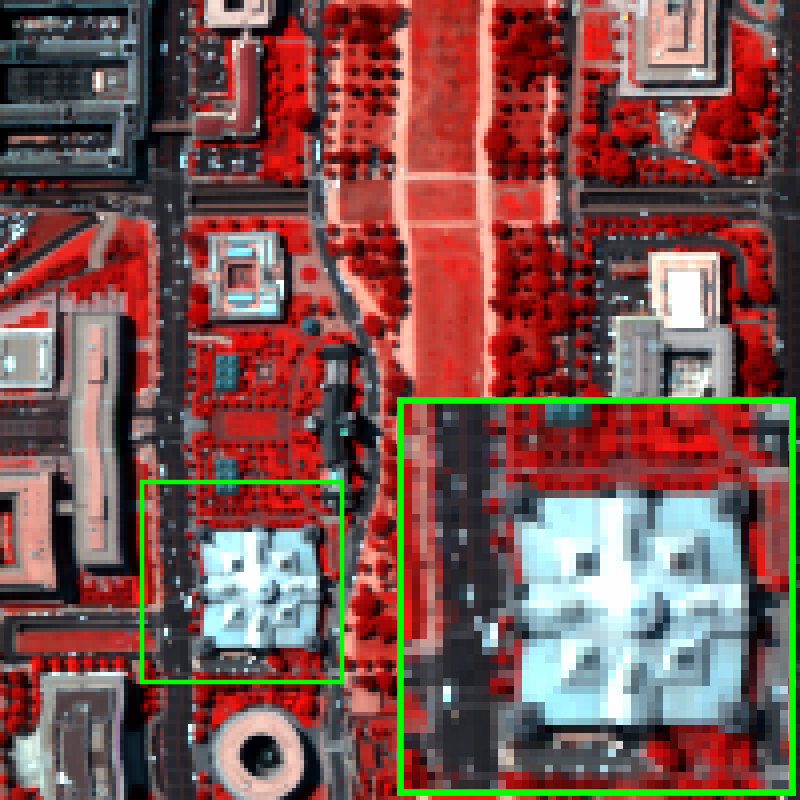
\includegraphics[width=\textwidth]{fichiers_latex/Chap1/figs/dcmall_out/clean.png}};
      \end{tikzpicture}
   \caption{Groundtruth}
\end{subfigure}
\hfill
\begin{subfigure}[b]{\figscale\textwidth}
      \begin{tikzpicture}[scale=\figscale]
        \node[anchor=south east,inner sep=0] at (0,0) {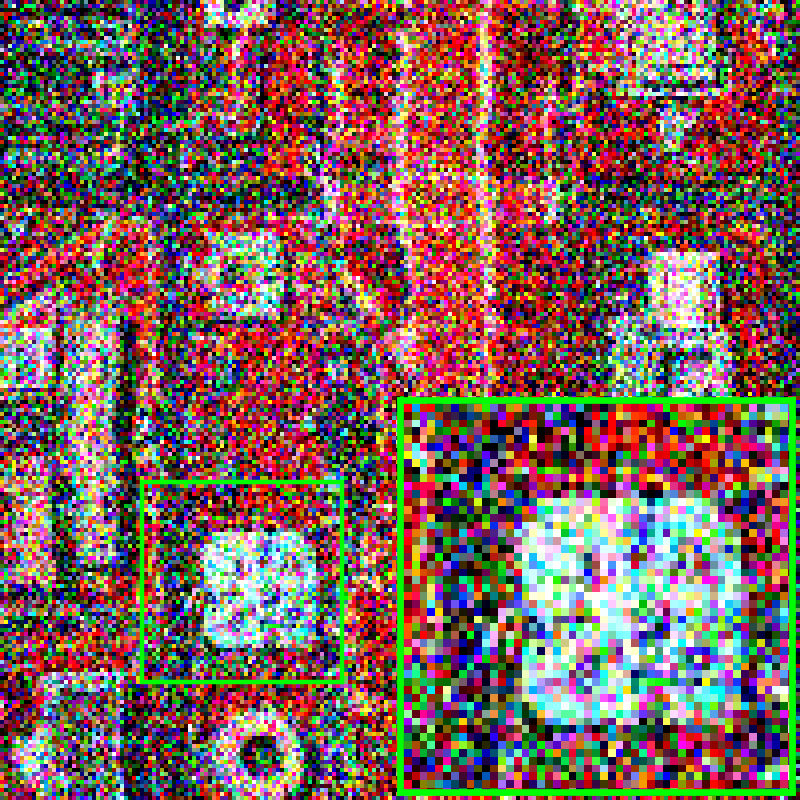
\includegraphics[width=\textwidth]{fichiers_latex/Chap1/figs/dcmall_out/in.png}};
      \end{tikzpicture}
   \caption{Noisy}
\end{subfigure}
\hfill
\begin{subfigure}[b]{\figscale\textwidth}
      \begin{tikzpicture}[scale=\figscale]
        \node[anchor=south east,inner sep=0] at (0,0) {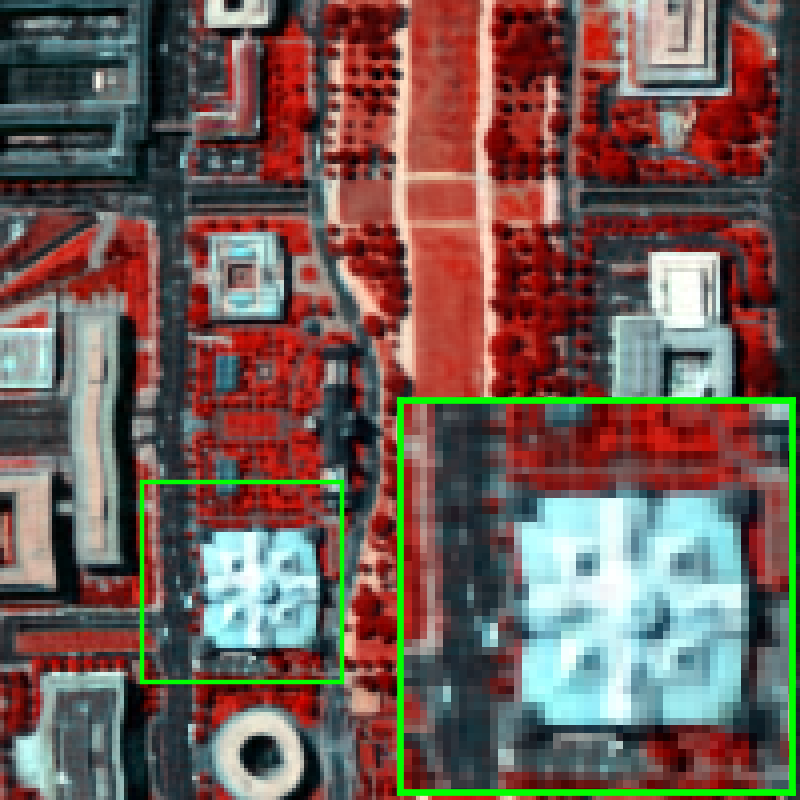
\includegraphics[width=\textwidth]{fichiers_latex/Chap1/figs/dcmall_out/llrt.png}};
      \end{tikzpicture}
   \caption{LLRT}
\end{subfigure}
\hfill
\begin{subfigure}[b]{\figscale\textwidth}
      \begin{tikzpicture}[scale=\figscale]
        \node[anchor=south east,inner sep=0] at (0,0) {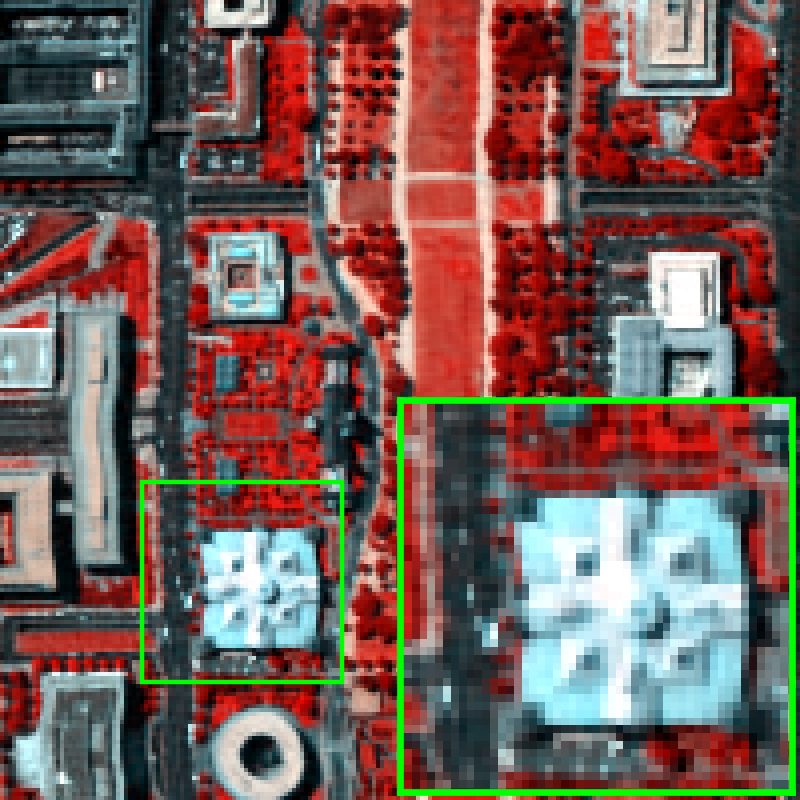
\includegraphics[width=\textwidth]{fichiers_latex/Chap1/figs/dcmall_out/ngmeet.png}};
      \end{tikzpicture}
   \caption{NGMeet}
\end{subfigure}
\\
\begin{subfigure}[b]{\figscale\textwidth}
      \begin{tikzpicture}[scale=\figscale]
        \node[anchor=south east,inner sep=0] at (0,0) {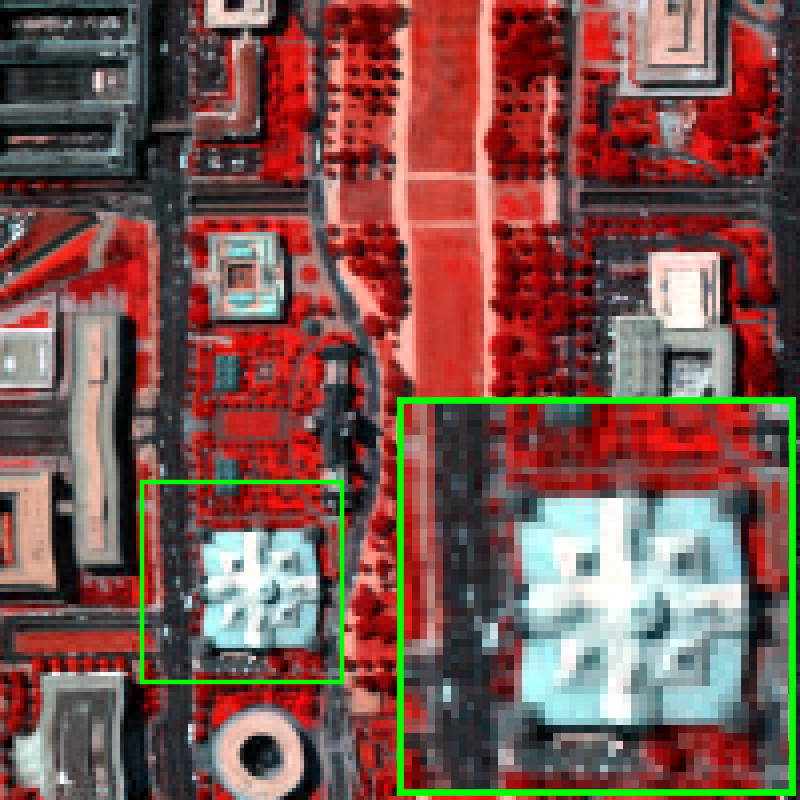
\includegraphics[width=\textwidth]{fichiers_latex/Chap1/figs/dcmall_out/glf.png}};
      \end{tikzpicture}
   \caption{GLF}
\end{subfigure} 
\hfill
\begin{subfigure}[b]{\figscale\textwidth}
      \begin{tikzpicture}[scale=\figscale]
        \node[anchor=south east,inner sep=0] at (0,0) {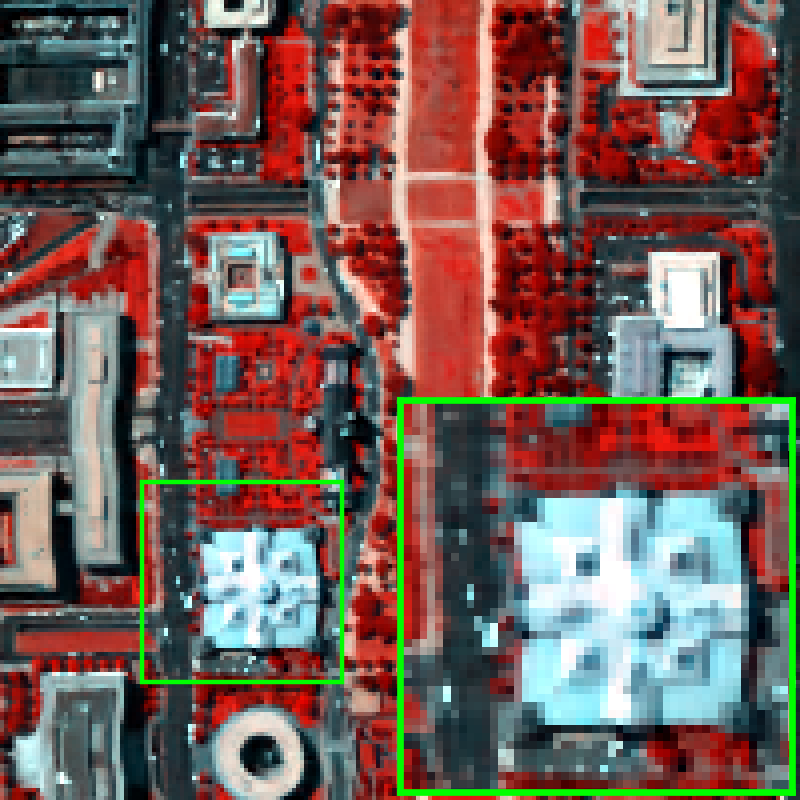
\includegraphics[width=\textwidth]{fichiers_latex/Chap1/figs/dcmall_out/smds.png}};
      \end{tikzpicture}
   \caption{SMDS-Net}
\end{subfigure}
\hfill
\begin{subfigure}[b]{\figscale\textwidth}
      \begin{tikzpicture}[scale=\figscale]
        \node[anchor=south east,inner sep=0] at (0,0) {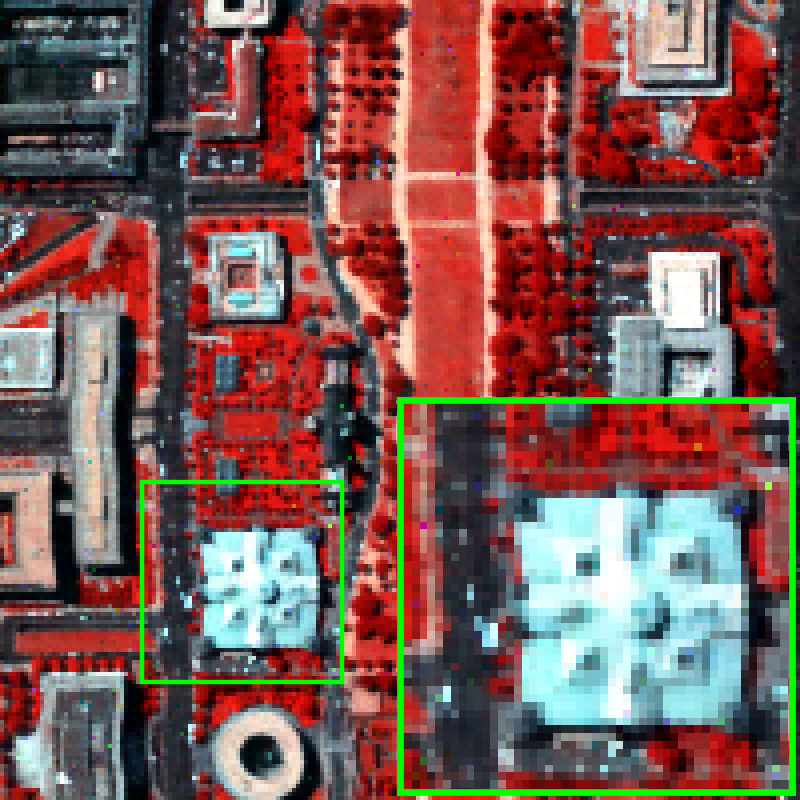
\includegraphics[width=\textwidth]{fichiers_latex/Chap1/figs/dcmall_out/qrnn.png}};
      \end{tikzpicture}
   \caption{QRNN3D}
\end{subfigure}
\hfill
\begin{subfigure}[b]{\figscale\textwidth}
      \begin{tikzpicture}[scale=\figscale]
        \node[anchor=south east,inner sep=0] at (0,0) {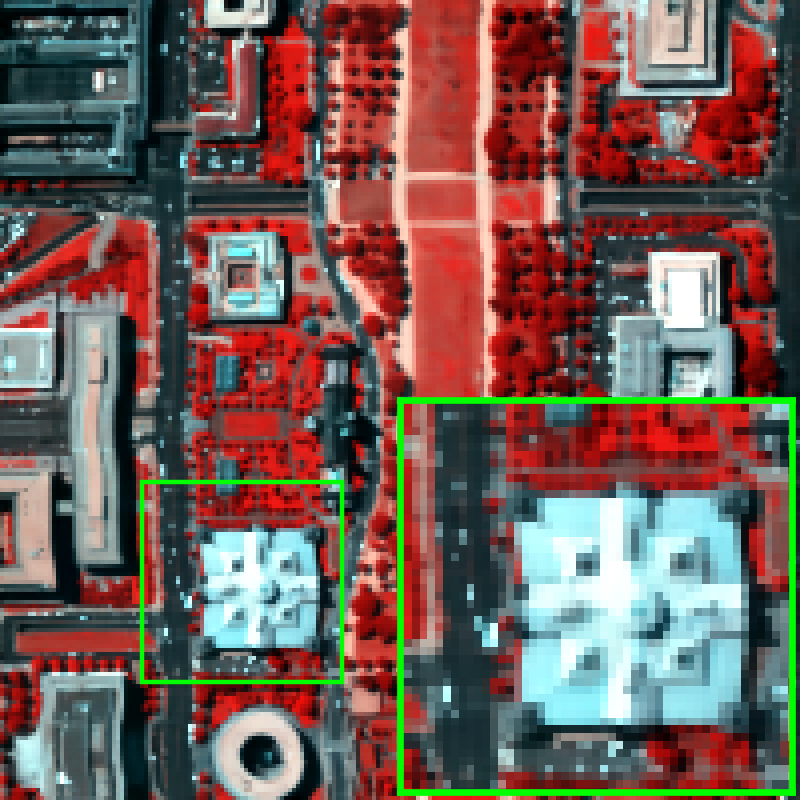
\includegraphics[width=\textwidth]{fichiers_latex/Chap1/figs/dcmall_out/t3sc.png}};
      \end{tikzpicture}
   \caption{T3SC}
\end{subfigure}


	\caption{Simulated Gaussian noise ($\sigma=100$) on DCMall}\label{fig:1}
\end{figure}

\begin{figure}[H]
	
\newcommand{\figscale}{0.24}

\begin{subfigure}[b]{\figscale\textwidth}
      \begin{tikzpicture}[scale=\figscale]
        \node[anchor=south east,inner sep=0] at (0,0) {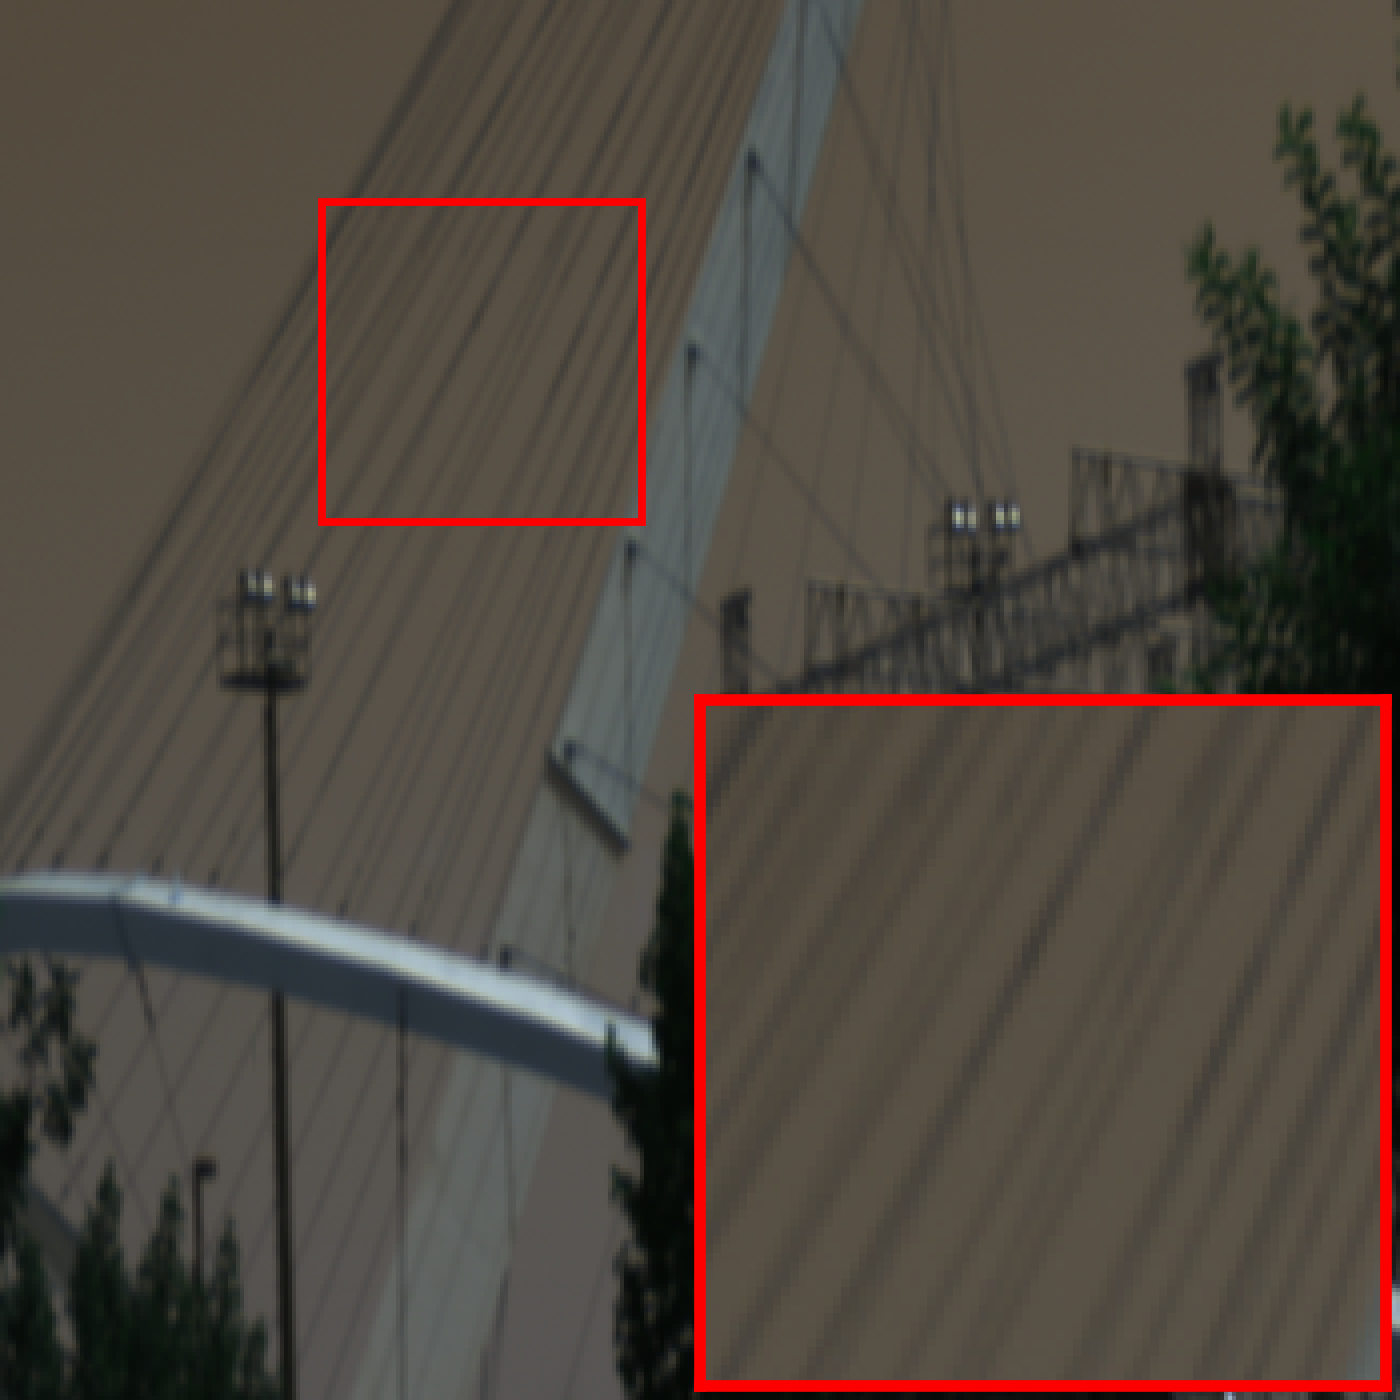
\includegraphics[width=\textwidth]{fichiers_latex/Chap1/figs/stripes/clean.png}};
      \end{tikzpicture}
   \caption{Groundtruth}
\end{subfigure}
\hfill
\begin{subfigure}[b]{\figscale\textwidth}
      \begin{tikzpicture}[scale=\figscale]
        \node[anchor=south east,inner sep=0] at (0,0) {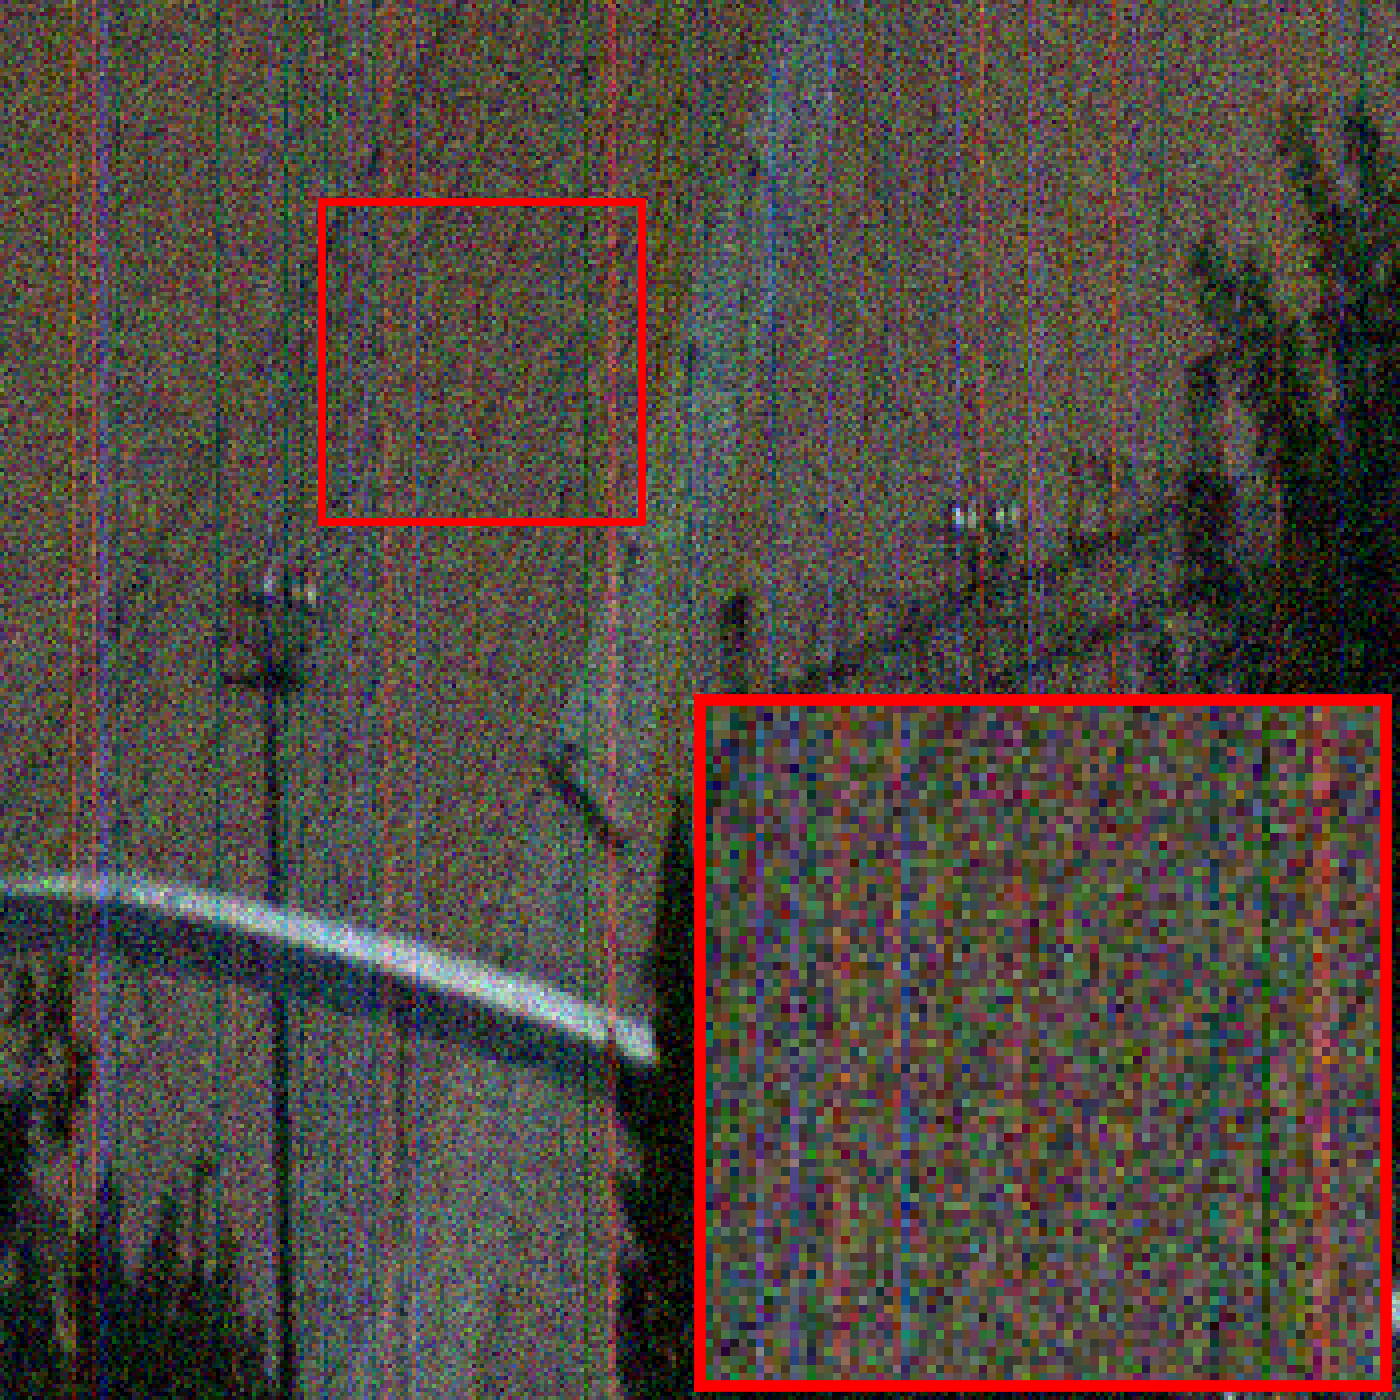
\includegraphics[width=\textwidth]{fichiers_latex/Chap1/figs/stripes/in.png}};
      \end{tikzpicture}
   \caption{Noisy}
\end{subfigure}
\hfill
\begin{subfigure}[b]{\figscale\textwidth}
      \begin{tikzpicture}[scale=\figscale]
        \node[anchor=south east,inner sep=0] at (0,0) {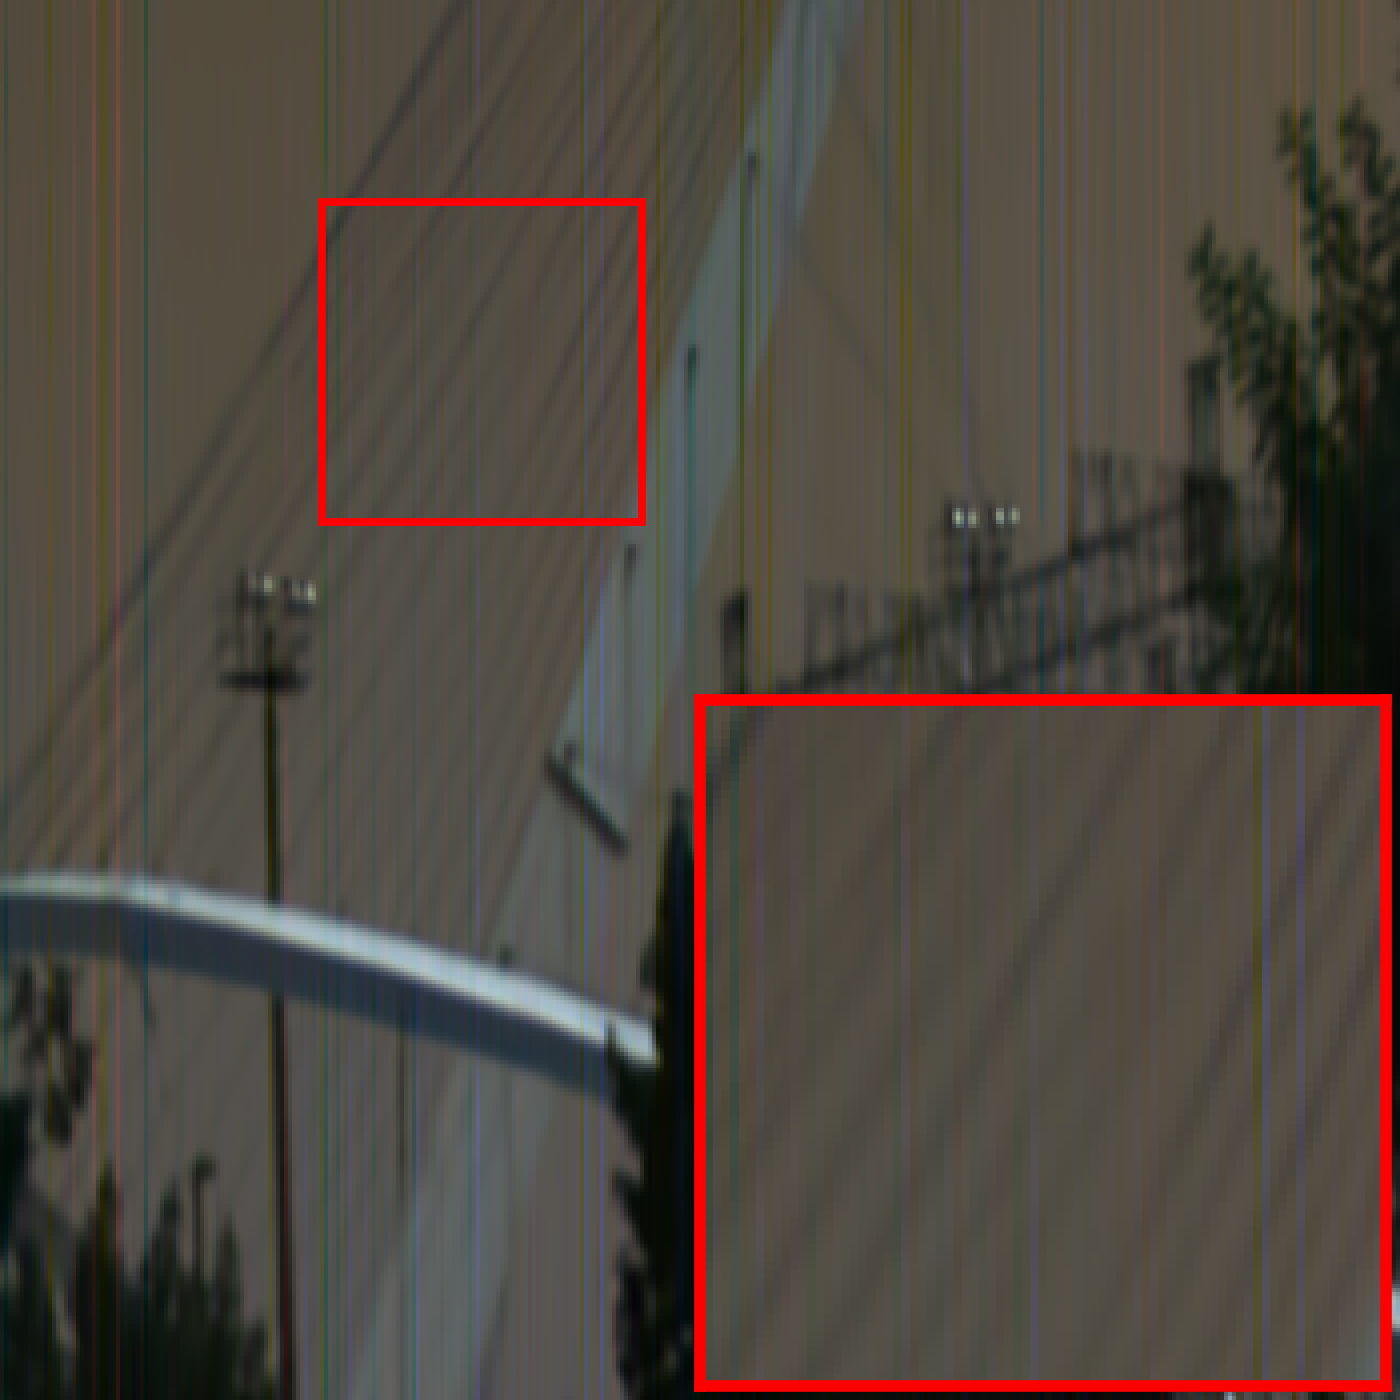
\includegraphics[width=\textwidth]{fichiers_latex/Chap1/figs/stripes/llrt.png}};
      \end{tikzpicture}
   \caption{LLRT}
\end{subfigure}
\hfill
\begin{subfigure}[b]{\figscale\textwidth}
      \begin{tikzpicture}[scale=\figscale]
        \node[anchor=south east,inner sep=0] at (0,0) {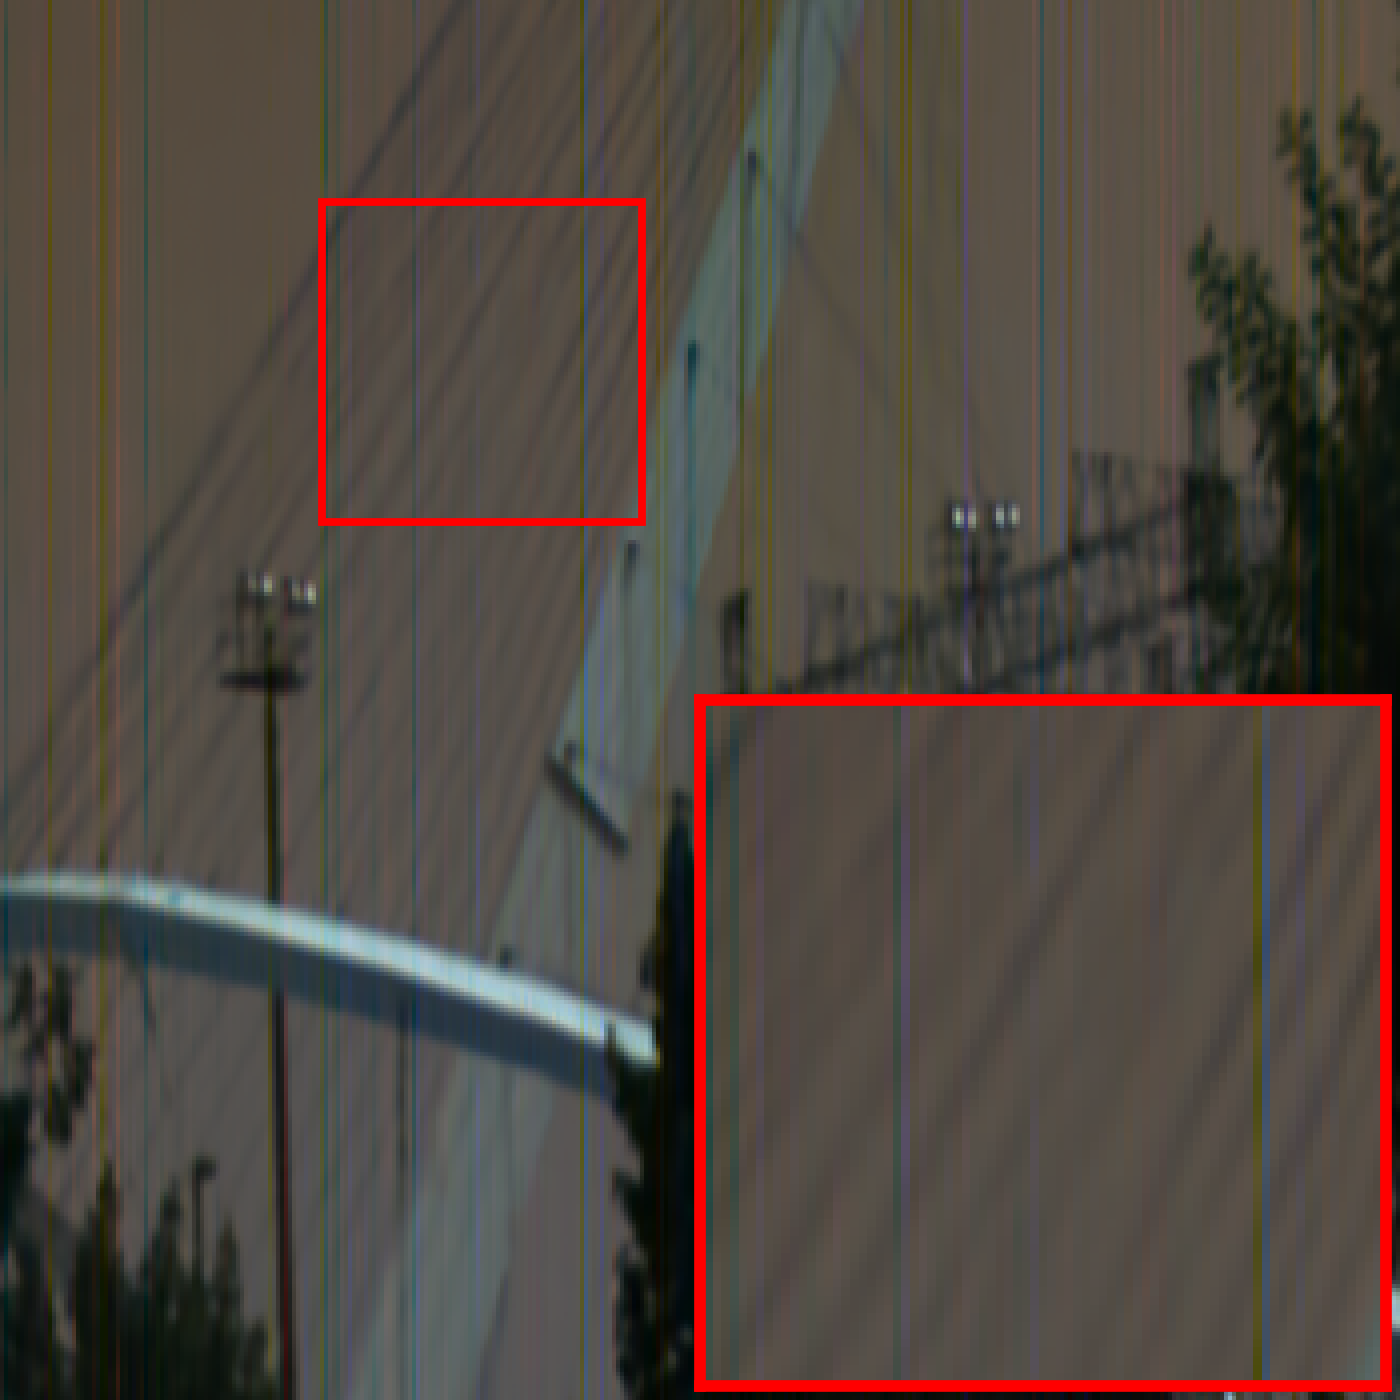
\includegraphics[width=\textwidth]{fichiers_latex/Chap1/figs/stripes/ngmeet.png}};
      \end{tikzpicture}
   \caption{NGMeet}
\end{subfigure}
\\
\begin{subfigure}[b]{\figscale\textwidth}
      \begin{tikzpicture}[scale=\figscale]
        \node[anchor=south east,inner sep=0] at (0,0) {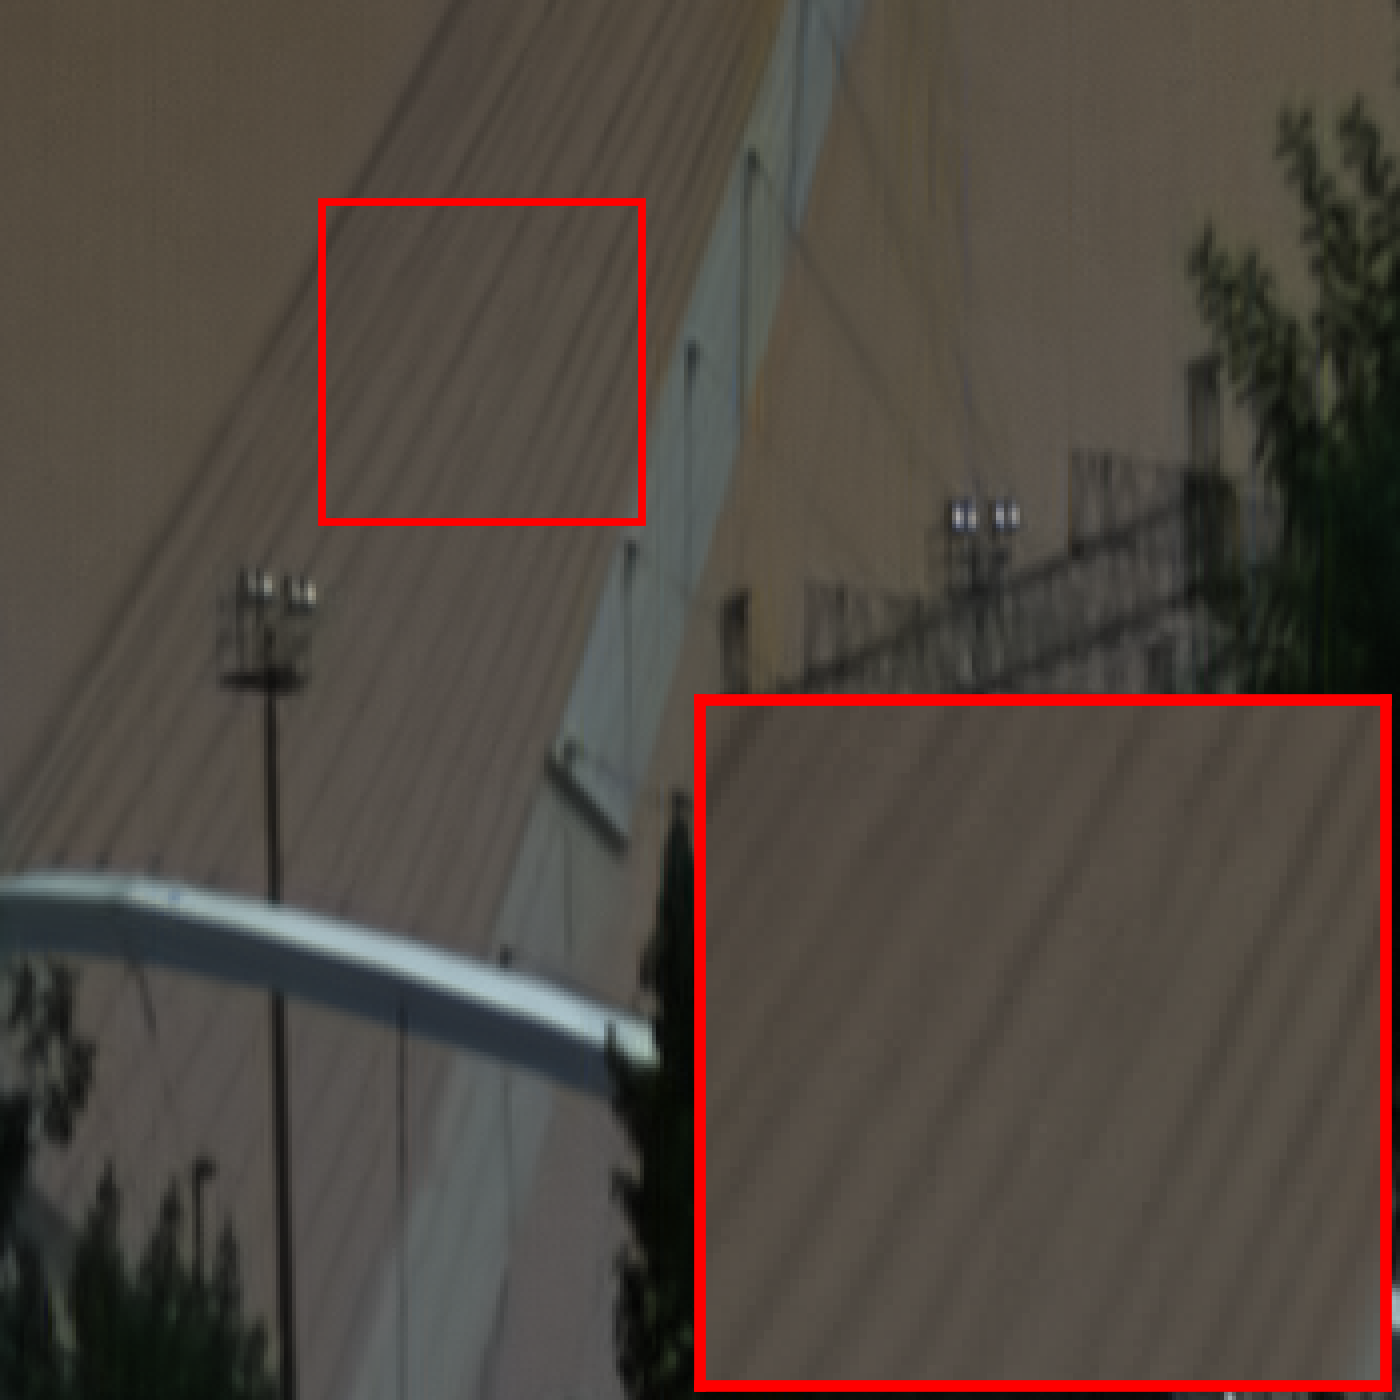
\includegraphics[width=\textwidth]{fichiers_latex/Chap1/figs/stripes/glf.png}};
      \end{tikzpicture}
   \caption{GLF}
\end{subfigure} 
\hfill
\begin{subfigure}[b]{\figscale\textwidth}
      \begin{tikzpicture}[scale=\figscale]
        \node[anchor=south east,inner sep=0] at (0,0) {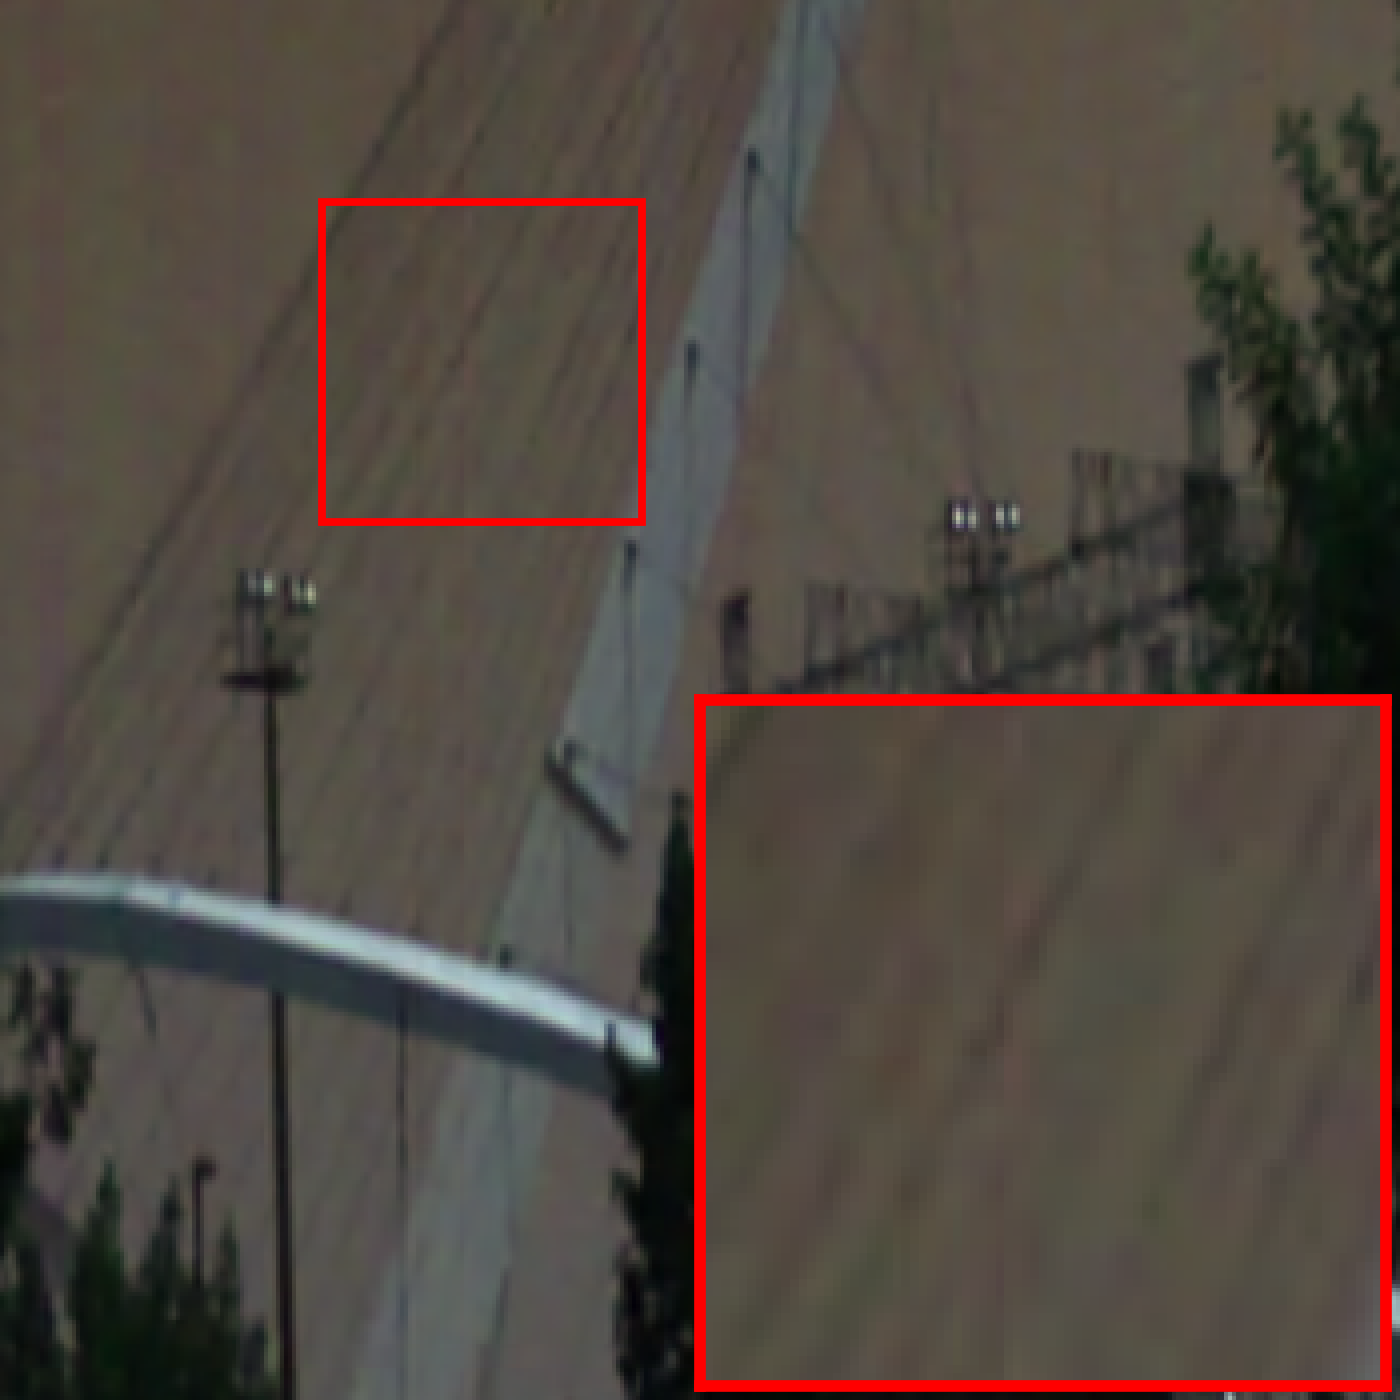
\includegraphics[width=\textwidth]{fichiers_latex/Chap1/figs/stripes/smds.png}};
      \end{tikzpicture}
   \caption{SMDS-Net}
\end{subfigure}
\hfill
\begin{subfigure}[b]{\figscale\textwidth}
      \begin{tikzpicture}[scale=\figscale]
        \node[anchor=south east,inner sep=0] at (0,0) {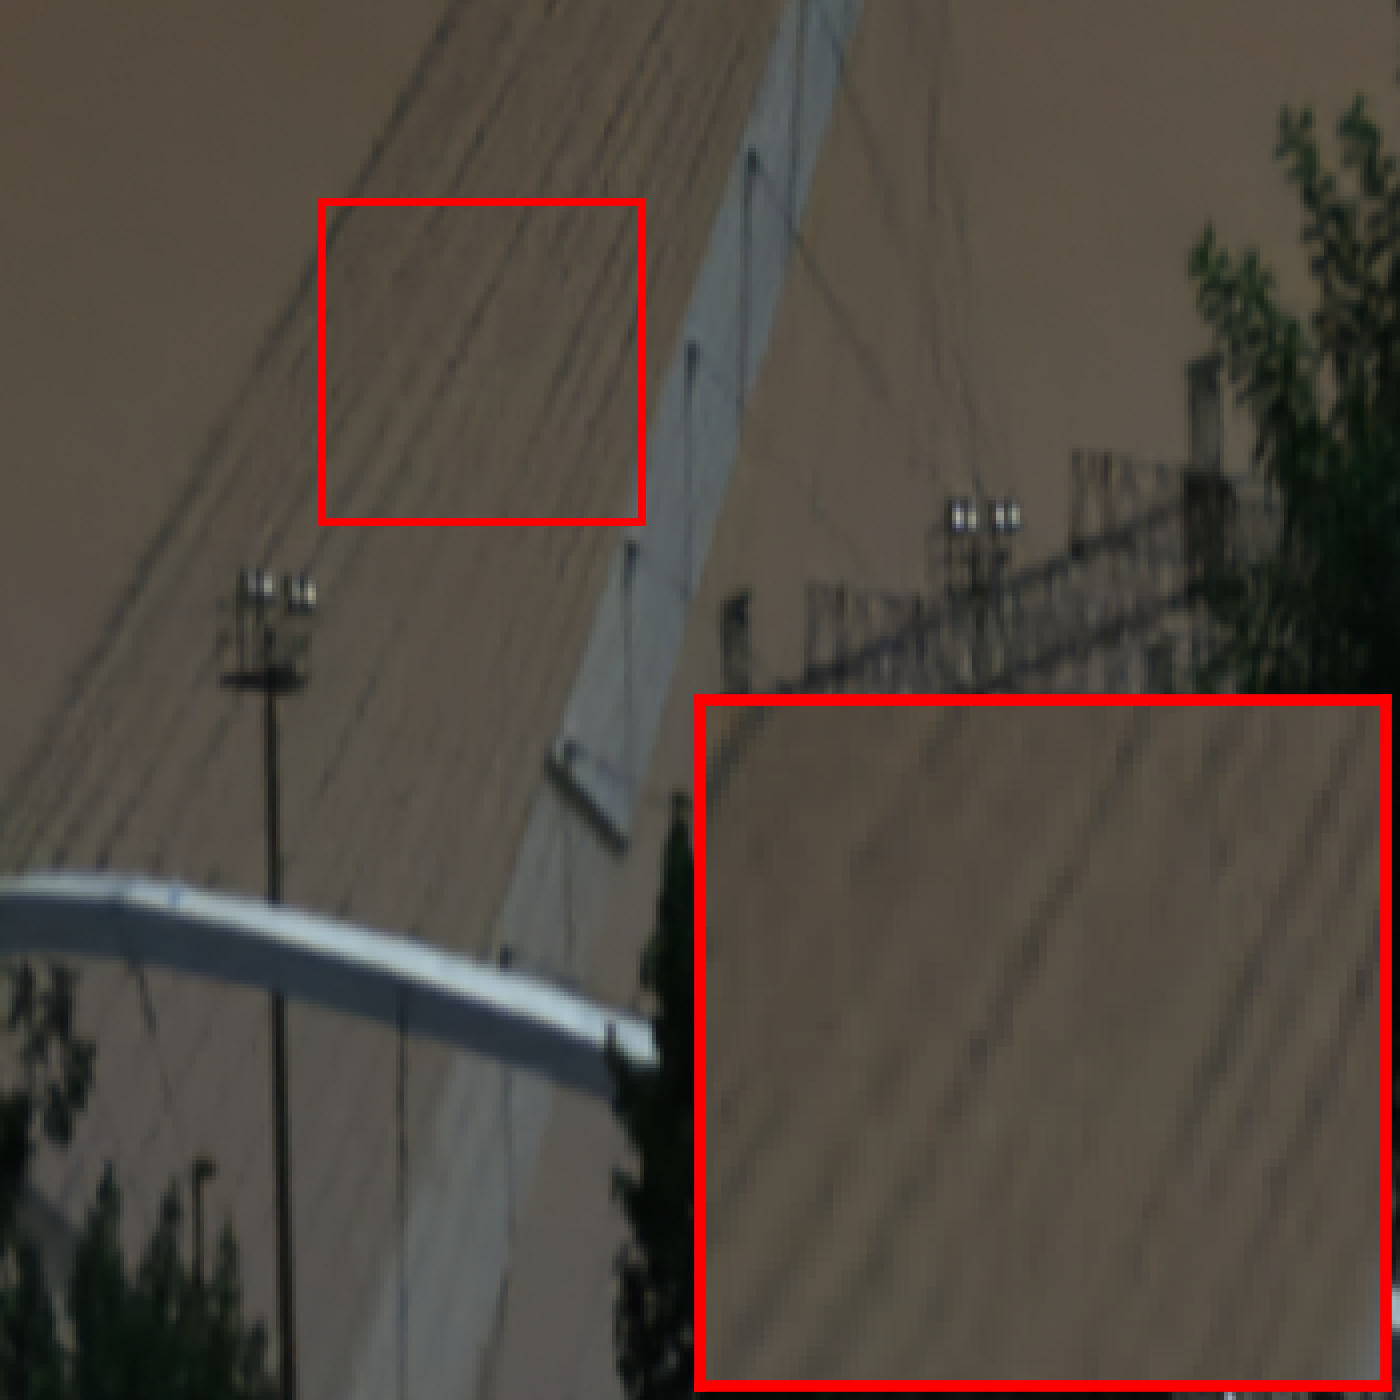
\includegraphics[width=\textwidth]{fichiers_latex/Chap1/figs/stripes/qrnn.png}};
      \end{tikzpicture}
   \caption{QRNN3D}
\end{subfigure}
\hfill
\begin{subfigure}[b]{\figscale\textwidth}
      \begin{tikzpicture}[scale=\figscale]
        \node[anchor=south east,inner sep=0] at (0,0) {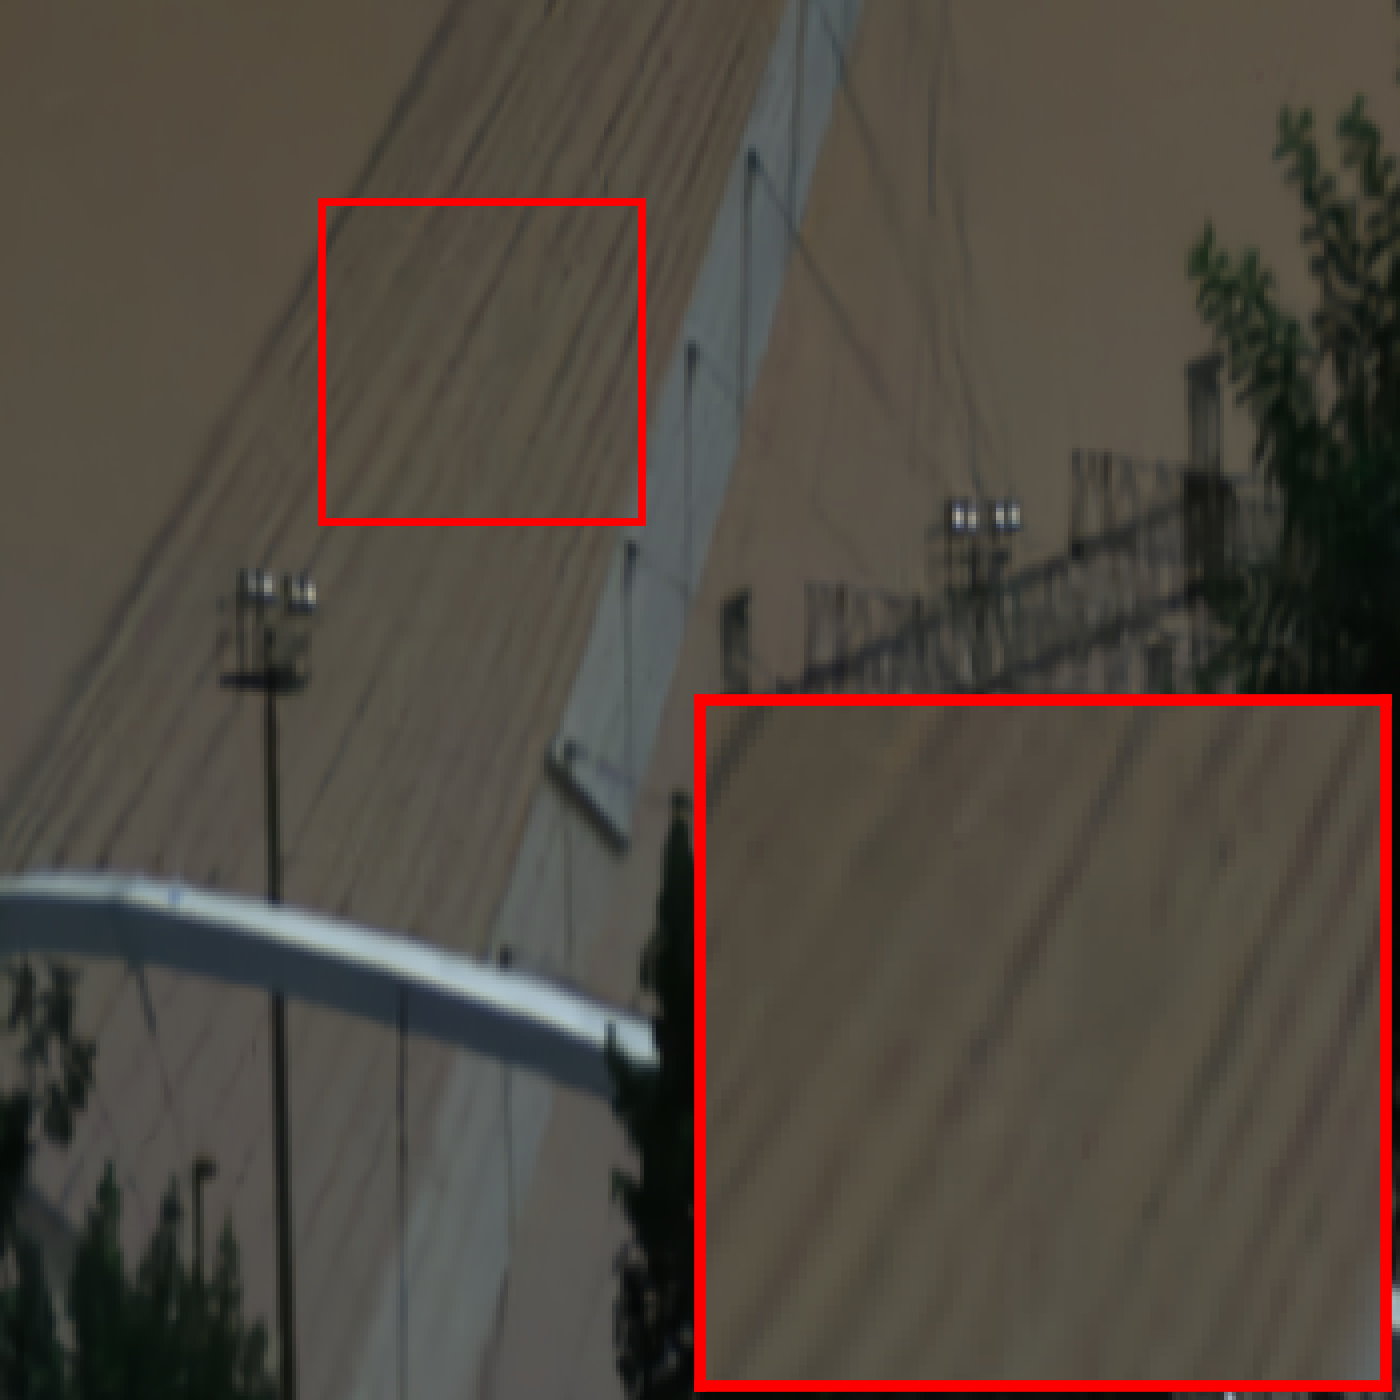
\includegraphics[width=\textwidth]{fichiers_latex/Chap1/figs/stripes/t3sc.png}};
      \end{tikzpicture}
   \caption{T3SC}
\end{subfigure}


	\caption{Visual results for the denoising experiment with stripes noise on ICVL with bands 9, 15, 28.}\label{fig:2}
\end{figure}


\section{GPU resources}

The total number of GPU hours involved in this project is around 19k hours on NVIDIA Tesla V100 16Go, including preliminary experiments, model design, final experiments and running baseline methods.